% Options for packages loaded elsewhere
\PassOptionsToPackage{unicode}{hyperref}
\PassOptionsToPackage{hyphens}{url}
\PassOptionsToPackage{dvipsnames,svgnames,x11names}{xcolor}
%
\documentclass[
  letterpaper,
  DIV=11,
  numbers=noendperiod]{scrreprt}

\usepackage{amsmath,amssymb}
\usepackage{iftex}
\ifPDFTeX
  \usepackage[T1]{fontenc}
  \usepackage[utf8]{inputenc}
  \usepackage{textcomp} % provide euro and other symbols
\else % if luatex or xetex
  \usepackage{unicode-math}
  \defaultfontfeatures{Scale=MatchLowercase}
  \defaultfontfeatures[\rmfamily]{Ligatures=TeX,Scale=1}
\fi
\usepackage{lmodern}
\ifPDFTeX\else  
    % xetex/luatex font selection
\fi
% Use upquote if available, for straight quotes in verbatim environments
\IfFileExists{upquote.sty}{\usepackage{upquote}}{}
\IfFileExists{microtype.sty}{% use microtype if available
  \usepackage[]{microtype}
  \UseMicrotypeSet[protrusion]{basicmath} % disable protrusion for tt fonts
}{}
\makeatletter
\@ifundefined{KOMAClassName}{% if non-KOMA class
  \IfFileExists{parskip.sty}{%
    \usepackage{parskip}
  }{% else
    \setlength{\parindent}{0pt}
    \setlength{\parskip}{6pt plus 2pt minus 1pt}}
}{% if KOMA class
  \KOMAoptions{parskip=half}}
\makeatother
\usepackage{xcolor}
\setlength{\emergencystretch}{3em} % prevent overfull lines
\setcounter{secnumdepth}{5}
% Make \paragraph and \subparagraph free-standing
\ifx\paragraph\undefined\else
  \let\oldparagraph\paragraph
  \renewcommand{\paragraph}[1]{\oldparagraph{#1}\mbox{}}
\fi
\ifx\subparagraph\undefined\else
  \let\oldsubparagraph\subparagraph
  \renewcommand{\subparagraph}[1]{\oldsubparagraph{#1}\mbox{}}
\fi


\providecommand{\tightlist}{%
  \setlength{\itemsep}{0pt}\setlength{\parskip}{0pt}}\usepackage{longtable,booktabs,array}
\usepackage{calc} % for calculating minipage widths
% Correct order of tables after \paragraph or \subparagraph
\usepackage{etoolbox}
\makeatletter
\patchcmd\longtable{\par}{\if@noskipsec\mbox{}\fi\par}{}{}
\makeatother
% Allow footnotes in longtable head/foot
\IfFileExists{footnotehyper.sty}{\usepackage{footnotehyper}}{\usepackage{footnote}}
\makesavenoteenv{longtable}
\usepackage{graphicx}
\makeatletter
\def\maxwidth{\ifdim\Gin@nat@width>\linewidth\linewidth\else\Gin@nat@width\fi}
\def\maxheight{\ifdim\Gin@nat@height>\textheight\textheight\else\Gin@nat@height\fi}
\makeatother
% Scale images if necessary, so that they will not overflow the page
% margins by default, and it is still possible to overwrite the defaults
% using explicit options in \includegraphics[width, height, ...]{}
\setkeys{Gin}{width=\maxwidth,height=\maxheight,keepaspectratio}
% Set default figure placement to htbp
\makeatletter
\def\fps@figure{htbp}
\makeatother
\newlength{\cslhangindent}
\setlength{\cslhangindent}{1.5em}
\newlength{\csllabelwidth}
\setlength{\csllabelwidth}{3em}
\newlength{\cslentryspacingunit} % times entry-spacing
\setlength{\cslentryspacingunit}{\parskip}
\newenvironment{CSLReferences}[2] % #1 hanging-ident, #2 entry spacing
 {% don't indent paragraphs
  \setlength{\parindent}{0pt}
  % turn on hanging indent if param 1 is 1
  \ifodd #1
  \let\oldpar\par
  \def\par{\hangindent=\cslhangindent\oldpar}
  \fi
  % set entry spacing
  \setlength{\parskip}{#2\cslentryspacingunit}
 }%
 {}
\usepackage{calc}
\newcommand{\CSLBlock}[1]{#1\hfill\break}
\newcommand{\CSLLeftMargin}[1]{\parbox[t]{\csllabelwidth}{#1}}
\newcommand{\CSLRightInline}[1]{\parbox[t]{\linewidth - \csllabelwidth}{#1}\break}
\newcommand{\CSLIndent}[1]{\hspace{\cslhangindent}#1}

\KOMAoption{captions}{tableheading}
\makeatletter
\makeatother
\makeatletter
\@ifpackageloaded{bookmark}{}{\usepackage{bookmark}}
\makeatother
\makeatletter
\@ifpackageloaded{caption}{}{\usepackage{caption}}
\AtBeginDocument{%
\ifdefined\contentsname
  \renewcommand*\contentsname{Table of contents}
\else
  \newcommand\contentsname{Table of contents}
\fi
\ifdefined\listfigurename
  \renewcommand*\listfigurename{List of Figures}
\else
  \newcommand\listfigurename{List of Figures}
\fi
\ifdefined\listtablename
  \renewcommand*\listtablename{List of Tables}
\else
  \newcommand\listtablename{List of Tables}
\fi
\ifdefined\figurename
  \renewcommand*\figurename{Figure}
\else
  \newcommand\figurename{Figure}
\fi
\ifdefined\tablename
  \renewcommand*\tablename{Table}
\else
  \newcommand\tablename{Table}
\fi
}
\@ifpackageloaded{float}{}{\usepackage{float}}
\floatstyle{ruled}
\@ifundefined{c@chapter}{\newfloat{codelisting}{h}{lop}}{\newfloat{codelisting}{h}{lop}[chapter]}
\floatname{codelisting}{Listing}
\newcommand*\listoflistings{\listof{codelisting}{List of Listings}}
\makeatother
\makeatletter
\@ifpackageloaded{caption}{}{\usepackage{caption}}
\@ifpackageloaded{subcaption}{}{\usepackage{subcaption}}
\makeatother
\makeatletter
\@ifpackageloaded{tcolorbox}{}{\usepackage[skins,breakable]{tcolorbox}}
\makeatother
\makeatletter
\@ifundefined{shadecolor}{\definecolor{shadecolor}{rgb}{.97, .97, .97}}
\makeatother
\makeatletter
\makeatother
\makeatletter
\makeatother
\ifLuaTeX
  \usepackage{selnolig}  % disable illegal ligatures
\fi
\IfFileExists{bookmark.sty}{\usepackage{bookmark}}{\usepackage{hyperref}}
\IfFileExists{xurl.sty}{\usepackage{xurl}}{} % add URL line breaks if available
\urlstyle{same} % disable monospaced font for URLs
\hypersetup{
  pdftitle={Nusses kogebog},
  pdfauthor={Christian},
  colorlinks=true,
  linkcolor={blue},
  filecolor={Maroon},
  citecolor={Blue},
  urlcolor={Blue},
  pdfcreator={LaTeX via pandoc}}

\title{Nusses kogebog}
\author{Christian}
\date{Invalid Date}

\begin{document}
\maketitle
\ifdefined\Shaded\renewenvironment{Shaded}{\begin{tcolorbox}[breakable, interior hidden, borderline west={3pt}{0pt}{shadecolor}, frame hidden, enhanced, sharp corners, boxrule=0pt]}{\end{tcolorbox}}\fi

\renewcommand*\contentsname{Table of contents}
{
\hypersetup{linkcolor=}
\setcounter{tocdepth}{2}
\tableofcontents
}
\bookmarksetup{startatroot}

\hypertarget{preface}{%
\chapter*{Preface}\label{preface}}
\addcontentsline{toc}{chapter}{Preface}

\markboth{Preface}{Preface}

This is a Quarto book.

To learn more about Quarto books visit
\url{https://quarto.org/docs/books}.

\bookmarksetup{startatroot}

\hypertarget{introduction}{%
\chapter{Introduction}\label{introduction}}

This is a book created from markdown and executable code.

See Knuth (1984) for additional discussion of literate programming.

\bookmarksetup{startatroot}

\hypertarget{summary}{%
\chapter{Summary}\label{summary}}

In summary, this book has no content whatsoever.

\bookmarksetup{startatroot}

\hypertarget{gris}{%
\chapter{Gris}\label{gris}}

\hypertarget{bacon-medisterpuxf8lse-i-airfryer}{%
\section{Bacon medisterpølse i
airfryer}\label{bacon-medisterpuxf8lse-i-airfryer}}

Medisterpølse vikles ind i bacon. 30 minutter i airfryer ved 180 grader.

\hypertarget{behuxe5ret-biker-puxf8lse}{%
\section{Behåret Biker pølse}\label{behuxe5ret-biker-puxf8lse}}

Eller Hairy Bikers' sausage casserole

1--2 tbsp sunflower oil: 1--2 tbsp sunflower oil 12 good-quality pork
sausages: 12 good-quality pork sausages 6 rashers rindless streaky
bacon, cut into 2.5cm/1in lengths: 6 rashers rindless streaky bacon, cut
into 2.5cm/1in lengths 2 onions, thinly sliced: 2 onions, thinly sliced
2 garlic cloves, crushed: 2 garlic cloves, crushed ½--1 tsp hot chilli
powder or smoked paprika: ½--1 tsp hot chilli powder or smoked paprika
400g tin chopped tomatoes: 400g tin chopped tomatoes 300ml/10fl oz
chicken stock: 300ml/10fl oz chicken stock 2 tbsp tomato purée: 2 tbsp
tomato purée 1 tbsp Worcestershire sauce: 1 tbsp Worcestershire sauce 1
tbsp dark muscovado sugar: 1 tbsp dark muscovado sugar 1 tsp dried mixed
herbs: 1 tsp dried mixed herbs 2 bay leaves: 2 bay leaves 3--4 fresh
thyme sprigs: 3--4 fresh thyme sprigs 100ml/3½fl oz red or white wine
(optional): 100ml/3½fl oz red or white wine (optional) 400g tin butter
beans or mixed beans, drained and rinsed: 400g tin butter beans or mixed
beans, drained and rinsed salt and freshly ground black pepper: salt and
freshly ground black pepper rice or rustic bread slices, to serve

\begin{verbatim}
Heat 1 tablespoon of the oil in a large non-stick frying pan and fry the sausages gently for 10 minutes, turning every now and then until nicely browned all over. Transfer to a large saucepan or a flameproof casserole dish and set aside.

Fry the bacon in the frying pan until starting to brown and crisp and then add to the dish with the sausages.

Add the onions to the frying pan and fry over a medium heat for 5 minutes until they start to soften, stirring often. You should have enough fat in the pan, but if not, add a little more oil. Add the garlic and cook for 2–3 minutes until the onions turn pale golden brown, stirring frequently.

Sprinkle over the chilli powder and cook together for a few seconds longer.

Stir in the tomatoes, stock, tomato purée, Worcestershire sauce, brown sugar and herbs. Pour in the wine, or some water if you’re not using wine, and bring to a simmer.

Tip the tomato mixture carefully into the pan with the sausages and bacon and return to a simmer. Reduce the heat, cover the pan loosely with a lid and leave to simmer very gently for 20 minutes, stirring from time to time.

Stir the beans into the casserole, and continue to cook for 10 minutes, stirring occasionally, until the sauce is thick.

Season to taste with salt and freshly ground black pepper and serve with rice or slices of rustic bread.
\end{verbatim}

\bookmarksetup{startatroot}

\hypertarget{kylling}{%
\chapter{Kylling}\label{kylling}}

\hypertarget{kyllingebrtyst-i-airfyer-med-estragoncreme}{%
\section{Kyllingebrtyst i airfyer med
estragoncreme}\label{kyllingebrtyst-i-airfyer-med-estragoncreme}}

\begin{itemize}
\item
  1 stk kyllingebryst
\item
  1 spsk olie
\item
  1 fed hvidløg revet
\item
  salt og peber
\item
  500 g bagekartofler
\item
  1 spsk olivenolie
\item
  2 kviste timian - finthakket
\item
  4 blade salvie - finthakket
\item
  2 kviste rosmarin - finthakket
\item
  salt og peber
\item
  1 dl græsk yoghurt
\item
  6 kviste frisk estragon - bladene
\item
  salt og peber
\end{itemize}

Vend kyllingen med olie, hvidløg, salt og peber

Vask kartoflerne og skær dem ud i både. Vend dem i olivenolie, og
krydderurterne. Fordel kartoffelbådene i bunden af airfryeren. Læg
kyllingebryst ovenpå Start fryeren ved 180 grader, og tilbered i 15
minutter Tag kyllingen op og lad den hvile i 5-10 minutter, mens
kartoflerne færdigsteger ved 200 grader Bland estragonen med yoghurt.
Smag til med salt og peber.

Skær kyllingen i skiver og anret med kartofler og creme.

\hypertarget{chicken-piccata}{%
\section{Chicken Piccata}\label{chicken-piccata}}

Fra VEEP

\begin{itemize}
\tightlist
\item
  Boneless, skinless chicken breasts
\item
  Salt \& pepper
\item
  Flour for dredging
\item
  Butter
\item
  Olive oil
\item
  Chicken stock
\item
  Skalotter
\item
  Hvidløg
\item
  Lemons, they brighten everything, including our Lemon Butter Chicken.
\item
  Kapers
\end{itemize}

Slice the chicken breasts horizontally---you'll need a sharp knife for
this, obviously! The reason you cut the chicken breast into thin pieces
is so that they can cook evenly during the pan-frying process. Thin
pieces of chicken mean that when the outside is crispy and perfectly
brown, the chicken will be cooked through. Magic! Dredge! Season the
chicken breast pieces, and then give them a nice coating of flour. For
whatever reason, kids really love to help out with this step. If they're
old enough to know to be careful with raw poultry, go ahead and
outsource this step to them! Fry! Fry the chicken cutlets in a
combination of olive oil and butter. The oil helps prevent the butter
from burning, plus, we love the flavor of both!

Our piccata sauce is simply a pan sauce, which means that we use the
good crispy, chicken-tinged buttery bits that are left in the skillet
after frying the chicken cutlets to make a sauce. Here's how to make
this lemony piccata sauce:

Sauté shallots and garlic in the pan drippings---i.e.~the leftover oil
and butter. Add stock! This is your chance to scrape up those tasty
brown bits from the bottom of the pan. Stir in more butter, plus the
requisite capers and lemon juice. Season with a little salt and pepper.
That's it! You made a pan sauce!

\hypertarget{kyllingetuxe6rte}{%
\section{Kyllingetærte}\label{kyllingetuxe6rte}}

\begin{itemize}
\tightlist
\item
  1 kylling
\item
  2 løg
\item
  5 fed hvidløg
\item
  3 porrer (to rækker)
\item
  4 gulerødder
\item
  4 stilke bladselleri, som vi udelader fordi Kristian ikke er fan af
  selleri.
\item
  1 pastinak eller persillerod. Stor.
\item
  1/4 kg champignons.
\item
  evt en håndfuld tørrede svampe. Ikke morkler eller den slags. Karl
  johan eksempelvis.
\item
  Timian
\item
  Laurbærblade 4 stk
\item
  ½ liter kraftig hønsefond
\item
  2 spsk mel - toppet
\item
  1 glas hvidvin (2½ dl)
\item
  2 dl fløde
\item
  Smør
\item
  Olivenolie
\item
  Butterdej
\end{itemize}

Fjern rygbenet fra kyllingen med en fjerkræsaks. skær brystbenet frit og
ud. krydr med salt og peber invendigt, og læg dyret på en rist med
kødsiden opad. Smør olivenolie på skindet og drys med sat. Bag den i
ovnen ved 200 grad i 45 minutter. Det går fint i en airfryer. Ryg og
brystben simrer i onden under låg i en halv times tid så vi får den smag
med. Fisk ben op og tilsæt de tørrede svampe til fonden. Lad dem trække
en 20 minutters tid. Hak løg - ikke for fint. Hak hvidløg - noget
finere. Skær rodfrugterne, porrene og sellerien (hvis du tager den med)
i mundrette stykker. Rens svampene og halver eller kvart dem. Olie og
smør i en stegegryde - når det er bruset af, først løg, lidt senere
hvidløg, og steg til de falder sammen, de skal ikke være helt
karameliserede. grøntsager og svampe tilsættes, sammen med timian og
laurbærbladene. Steg det hele til de tager en smule farve og
rodfrugterner er en smule møre. Drys mel over og bag af. Tilsæt fond og
hvidvin lidt af gangen og kog til det tykner. Tilsæt fløde og lad det
simre yderligere et par minutter. Der kan jævnes lidt mere med maizena.
Det skal være ret tykt.

Når dyret er færdig i ovnen tages det ud og køler nok af til at man kan
arbejde med det. Evt. sprødt skind tages af og skæres i små stykker. Al
snask fra bradepanden skrabes over i gryden. Pil kødet fra dyret, og sær
i mindre tern. Kom det i stuvningen og smag til med salt og peber. Fisk
laurbærblade og timianstilke (hvis du brugte frisk timian) op. Smid også
kyllingeskindet i.

Kom stuvningen i dyb tærteform eller lignede og lad det køle af. Rul
butterdej ud (hvis ikke den kommmer i plade). Pensl kanten på formen med
æg og læg butterdej på som låg. Pensl låget med æg, og skær et snit i
midten af låget, så damp kan slippe ud. Bag i ca 35 minutter ved 200
grader. Lad den hvile ti minutter inden servering.

\hypertarget{hverdagskylling-med-kremede-svampe}{%
\section{Hverdagskylling med kremede
svampe}\label{hverdagskylling-med-kremede-svampe}}

Fra food52

\begin{itemize}
\tightlist
\item
  ½ kg svampe
\item
  4 spsk smør
\item
  ½ kg kyllingebryster - Oprindeligt var det 1 kg
\item
  2½ dl piskefløde (eller madlavningsfløde)
\item
  2 spsk dijon sennep
\item
  finthakket purløg
\end{itemize}

Rens svampene, skær halvdelen i skiver, og resten i kvarter.

\begin{itemize}
\tightlist
\item
  Smelt 2 spsk smør,
\item
  tilføj svampene, steg dem 10-15 minutter, til de begynder at
  karamelisere.
\item
  Halver kyllingebrysterne på langs, og bank dem med kødhammeren, ca 1/4
  tomme så - 40 millimeter?
\item
  dub dem af, og krydr med salt og peber.
\item
  Giv svampene lidt salt og peber, deglacer med 1/3 cup vand.
\item
  Smelt resten af smørret, steg kyllingerne. Smid gerne en bøfpresse
  ovenpå dem.
\item
  Bland fløde og sennep. Rør dem i svampene, og kog under omrøring til
  den tykner. Smag til med salt, peber og sennep.
\item
  Saml - kylling overhældes med svamep. Vi serverer med ris.
\end{itemize}

\hypertarget{onepot-chicken-rice}{%
\section{Onepot chicken \& rice}\label{onepot-chicken-rice}}

Fra noma

\begin{itemize}
\item
  60 g olie
\item
  4 kyllige lår uden ben, med skind
\item
  salt
\item
  140 gram løg finthakket
\item
  3 fed hvidløg smadret
\item
  15 g tomatpasta
\item
  60 g hvid miso
\item
  15 g røget paprika
\item
  80 g røget svampe garum
\item
  600 g grøntsagsbouillon
\item
  10 g salt
\item
  200 g ris
\item
  10 g persille
\item
  200 g mayonaise
\item
  1 fed hvidløg - revet.
\end{itemize}

Olie varmes op i sautepanden ved middel varme. Krydr kyllingerne med
generøse mængder salt. Når olien simrer, brunes kyllingen på skindsiden
(men kun skindsiden), til den er mørkebrun og sprød. Det skal tage ca. 4
minutter. Fjern kyllingerne fra panden. Skru ned til lav varme. tilsæt
løg og hvidløg. Steg til løgene er klare. rør tomatpastaen i og steg ca.
5 minutter til tingene er rustent brune. Tilsæt bouillon, salt, røget
svampe garum, parpirka og miso. Øg temperatren til høj. Rør for at
blande.

Når væsken koger, tilsæt risene og rør så de er jævnt fordelt. Her fra
skal risene ikke røres!

Skru ned for varmen, og lad den simre. tilføj kyllingerne til gryden,
med den rå side ned. (så ved stegningen er det kun på skindsiden at den
skal steges!) Når duften af brændte ris kan mærkes - efter ca. 20-25
minutter er vi ca. færdige. tag af varmen, og lad hivle i 5 minutter.
pynt med hakket persille.

Bland mayo med hvidløg og bland godt.

Server portioner af ris på tallerken - husk at få det sprøde let brændte
lag med. Kylling på toppen. Top yderligere med hvidløgsmayo.

\hypertarget{pollo-orzo}{%
\section{Pollo orzo}\label{pollo-orzo}}

One pot. Og relativt hurtig.

\begin{figure}

{\centering 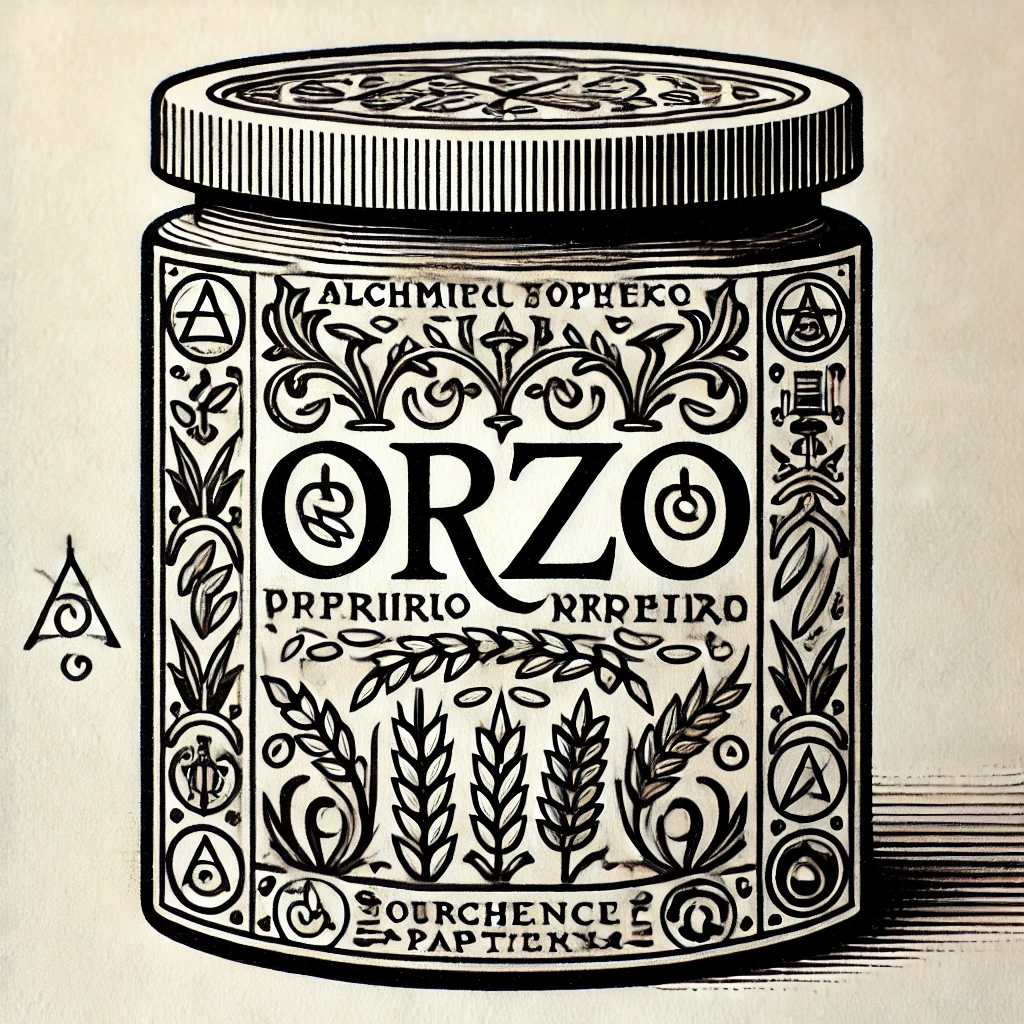
\includegraphics{rmds/images/orzo.png}

}

\caption{orzo}

\end{figure}

Orzo er de der små rislignende pastating.

\begin{itemize}
\tightlist
\item
  Kyllingestykker. Helst med ben. En samling lår er fint.
\item
  3 fed hvidløg
\item
  2 tsk salt
\item
  peber
\item
  1½ liter vand
\item
  \textasciitilde½ liter kyllingefond.
\item
  En dåse hakkede tomater
\item
  1 løg eller to hvis det er et lille løg
\item
  340 gram orzo pasta
\item
  persille
\end{itemize}

Brun killingerne i olie/smør/andefedt/margarine ca. 5 minutter på hver
side.

Tag killingerne op, og brun pastaen let i fedtstoffet.

Tilsæt finthakket løg og klar løgene. Smid finthakket hvidløg i til
sidst.

Læg killingerne tilbage i panden.

Hæld fond og tomater over.

Låg på, og lad simre 10-15 minutter, afhængig af orzo type og killing.
Pastaen skal være al dente, killingen skal være gennemstegt/kogt.

Tag gryden af varmen, og lad den hvile i 5 minutter. Orzoen skal gerne
absorbere stort set al væden. Hvis det skal være ekstra festligt, så
hæld persille over.

\hypertarget{kylling-med-ris.-i-uxe9n-gryde-ok-sauterpande}{%
\section{Kylling med ris. I én gryde (ok,
sauterpande)}\label{kylling-med-ris.-i-uxe9n-gryde-ok-sauterpande}}

Når man både er ham der laver mad, og ham tager det meste af opvasken -
så er man da et fjols hvis ikke man foretrækker opskrifter der giver
minimalt med opvask.

\begin{itemize}
\tightlist
\item
  4 stykker kylling (helst med skind og ben)
\item
  Olivenolie
\item
  1 løg (hakkes fint)
\item
  3 fed hvidløg (ligeledes finthakket)
\item
  1 tsk spidskommen (stødt)
\item
  ½ tsk koriander (stødt)
\item
  Saft af 1 øko-citron
\item
  Lidt af skallen fra 1 øko-citron
\item
  1 tsk timian (tørret)
\item
  3 dl ris
\item
  5-6 dl kyllingfond. Eller grøntsagsbouillon - afhængig af hvad der nu
  lige er i køkkenskabet
\end{itemize}

Kyllingen drysses med salt og peber og brunes af i sauterpanden i olien.
Kyllingen tager en pause på en tallerken, og løgene steges klare og
bløde. Resten af ingredienserne hældes i panden, der røres godt rundt,
og kyllingerne vender tilbage. Lad simre under låg i ca 5 minutter.

Dernæst tages låget af, og panden sættes i ovnen (forvarmet!) ved 200
grader i 12-13 minutter. Tiden afgøres af hvornår risene er møre og
kyllingen er gennembagt. Sæt låg på, og lad kødet hvile en 4-5 minutter.
Drys evt med friske krydderurter ved serveringen.

\hypertarget{kylling-med-kartofler-og-whiskeysovs}{%
\section{Kylling med kartofler og
whiskeysovs}\label{kylling-med-kartofler-og-whiskeysovs}}

Forestil dig en gryde. Med ovnstegte kartofler, i små stykker, stegt
kylling, i små stykker. Altsammen kærligt omsvøbt af whiskeysovs. Mums.

Den findes i flere udgaver ude på nettet. Her er min.

\begin{itemize}
\tightlist
\item
  500 gram kyllingeinderfilletter
\item
  700 gram kartofler
\item
  700 gram gulerødder
\item
  Olie
\item
  En pakke bacon
\item
  Et glas champignon
\item
  2½ dl fløde
\item
  Mælk (nok 2½ dl. men ``nok'')
\item
  Smør (rigeligt)
\item
  1½ spsk mel
\item
  2 tsk karry
\item
  3 tsk paprika
\item
  1 dl BBQ-sovs
\item
  4 spsk whisky
\item
  Salt og peber
\item
  Purløg
\end{itemize}

Kartofler og gulerødder skrælles og skæres i mindre stykker. Størrelsen
må godt være ensartet, så når gulerødderne ikke er alt for tykke, og
skæres ud i ca. 1½ cm lange stykker - så følger kartoflerne med.

De vendes i olie, salt og peber, og smides i ovnen ved 180 grader
varmluft. I min ovn er de ved at være møre og har fået lidt farve efter
45-50 minutter.

Mens de er derinde, steges en pakke bacon (skåret i stykker). Baconen
tages fra og kyllingefilletterne, også skåret i stykker, her i ca. samme
størrelse som grøntsagerne, steges. Kyllingen tages fra, og nu steges
champignonerne (normalt ville jeg bruge friske champignons. Og nok ½ kg.
Men vores pandemilagre skal jo bruges). Når de har fået hvad de skal
have, drysses mel og krydderier over. Bag melet igennem, og tilsæt
fløden lidt af gangen. Tænk opbagt sovs.

Tilsæt whiskey og BBQ-sovs. Og smag til med salt og peber. Der skal nok
tilsættes i hvert fald 2½ dl mælk. Måske lidt mere.

Når grøntsagerne er færdige i ovnen, smides de i gryden, sammen med
kyllingen og baconen. Varm igennem, og server med purløg.

Lækkert!

\hypertarget{kylling-i-karry-med-gruxf8nt}{%
\section{Kylling i karry med grønt}\label{kylling-i-karry-med-gruxf8nt}}

Her i huset gider vi ikke høre på vås om hvor slemt det er at kvinder
står med rengøringen, madlavningen og så videre.

Her i huset er det nemlig manden der står for alt det. Det hjælper
selvfølgelig at vi er to mænd og ingen kvinder i lejligheden\ldots{}

Og ikke alene er det manden der står for madlavningen. Det er mig. Jeg
har så også tjansen med indkøb, rengøring og oprydning. Så maden skal
kunne laves hurtigt. Samtidig med at jeg ikke vil gå på (ret meget)
kompromis med kvaliteten.

Derfor her, en hurtig opskrit på kylling i karry. Og grønt.

500 g kyllingefilet. Gerne inderfileten 1-2 tsk karrypasta. Eller alm.
karry. Efter bebov. 5 spsk sojasovs 500 g grønsagsblanding fra frost 1
ds kokosmælk

Brun kyllingerne i en wok-pande. Drys karry og soja over. Steg til
kyllingen er gennemstegt. Tilsæt grønsagsblandingen og rør rundt et par
minutter Tilsæt kokosmælk Når grøntsagerne er varmet igennem, smages til
med salt, peber og mere karry. Server med kogte ris.

Hurtigt og enkelt.

\hypertarget{kylling-og-spidskuxe5l}{%
\section{Kylling og spidskål}\label{kylling-og-spidskuxe5l}}

Vi prøver virkelig at spise grønnere. Og det her er en af de opskrifter
der er, om ikke grøn, så grønnere, end hvad der ellers er i fast
rotation. Den er også hurtig, og det er godt.

\begin{itemize}
\tightlist
\item
  400 g kyllingeinderfilet
\item
  salt og peber
\item
  Olie
\item
  2 fed hvidløg
\item
  1 spidskål
\item
  4 gulerødder
\item
  2 spsk sojasovs
\item
  2 spsk citronsaft
\item
  2 tsk honning - helst flydende
\end{itemize}

Kyllingenstykkerne brunes i olien. Jeg bruger normalt wokken. Hak
hvidløgene og lad dem stege lidt med - lad dem ikke blive brune!
Spidskål og gulerødder - strimlet - tilsættes, og steger med 3-4
minutter. Rør soja, citronsaft og honning sammen og tilsæt det til
wokken. Varm igennem, og smag til med salt, peber og evt mere soja.
Server med ris eller groft brød.

\hypertarget{simpel-mad-1.1}{%
\section{Simpel mad 1.1}\label{simpel-mad-1.1}}

Så bliver det ikke meget enklere.

Man tager 6-8 peberfrugter, hold dig til gule og røde. Orange kan også
bruges, men det gør ingen forskel i hvordan retten ser ud når den er
færdig.

Rens og skær dem ud i store tern.

Smid dem i en gryde, læg 8 kyllingelår oven på. Andre dele af kyllingen
kan også bruges, men helst med skind og ben af hensyn til smagen.

Giv det hele et drys salt, og sæt det på komfuret. Rør regelmæssigt de
første ti minutters tid. Peberfrugterne afgiver hurtigt store mængder
væske, og falder sammen. Læg låg på, og lad det simre en tre kvarters
tid. Måske lidt længere afhængig af hvilke dele af kyllingen der røg i
gryden.

Og vupti, så er retten færdig. Jeg aner ikke hvad jeg vil kalde den, men
kæresten, der normalt ikke er meget for peberfrugter, var ret
begejstret. Hvis man absolut vil, kan man give den en smule maizena, men
det synes jeg er synd.

Med lidt held er der væske til rest. Det gør sig ubeskriveligt godt i
kødsovs har vi erfaring for.

\hypertarget{simpel-mad-1.1.1}{%
\section{Simpel mad 1.1.1}\label{simpel-mad-1.1.1}}

En videreudvikling af peberfrugtkyllingen står og hygger sig på blusset
netop nu.~

Tomat går godt med kylling. Tomat går også ok med peberfrugt. Så de tre
røde og tre gule peberfrugter, og de fire kyllingelår (med rygstykke),
er blevet suppleret med ½ kg cherrytomater.

De dufter fantastisk allerede inden de kommer i gryden, nu ser vi
hvordan det går med smagen. Næste videreudvikling kommer nok til at ske
med bacon. Bacon går godt sammen med hvad som helst\ldots{}

\hypertarget{simpel-mad-3}{%
\section{Simpel mad 3}\label{simpel-mad-3}}

Meget passende har retten tre ingredienser:

\begin{itemize}
\tightlist
\item
  4 kyllingebryster
\item
  4 tsk sød sennep
\item
  1 kop knuste ristede løg
\end{itemize}

Kyllingen smøres ind i sennep, og paneres i ristede løg.~

Lægges på folie i oven, nok gerne et ovnfast fad, i 20-25 minutter ved
190 grader.

\bookmarksetup{startatroot}

\hypertarget{ko}{%
\chapter{Ko}\label{ko}}

Ko-opskrifter.

\hypertarget{boeuf-saute-stroganoff}{%
\section{Boeuf saute stroganoff}\label{boeuf-saute-stroganoff}}

Pricernes opskrift.

\begin{itemize}
\tightlist
\item
  800 g oksefilet
\item
  3-4 spsk edelsuss paprika
\item
  3-4 løg
\item
  2 spsk smør
\item
  300 g champignon (eller andre svampe)
\item
  5-6 tykke skiver bacon
\item
  2 spsk tomatpure
\item
  ½ l fløde
\item
  salt og peber
\end{itemize}

Kødet skæres i strimler på størrelse med en lillefinger. Det pudres med
paprikaen. Svampene skæres i tynde skiver og steges i lidt smør. Fisk
dem op og læg dem til side. Løgene hakkes og klares i mere smør. Når de
er klarede fiske de op og lægges til side. Bacon skæres i mindre
strimler og steges til de er gyldne - men ikke for sprøde. Fisk også dem
op. I det fedt der er tilbage i gryden brunes kødstrimlerne over ret
kraftig varme. Men pas på paprikaen brænder let på.

Tilsæt tomatpureen og steg den lidt på panden.

Alt det der var lagt til side kommes op i gryden igen. Fløden hældes på,
og der koges til det tykner. Smag til med salt, peber og evt. lidt mere
paprika.

Pricerne ville servere fritter. Mos eller ris er også glimrende.

\hypertarget{stifatho}{%
\section{Stifatho}\label{stifatho}}

Det har sikkert været med ged eller lam snarere end ko. Men her i huset
laves det med ko. 800 g oksetykkam eller lignedne 15 hele løg (lidt
afhængig af deres størrelse) 4 fed hvidløg 5 laurbærblade 2 spsk
tomatpure 4 dl rødvin ½ kalve eller okse boullion olivenolie, salt og
peber

Puds kødet af og skær det i store tern - 2-4 cm på hver led. Steg det
afpudsede af i en separat gryde, og hæld bouillion over - lad det simre.
Kødet brunes godt af i stegegryden, gerne af nogle omgange. Pil løgene
og smid dem i gyrden. Pil hvidløgene og mos dem. De skal også i gryden.
Laurbærbladene kommer også i, og så lader vi det hele få varmen i
gryden, før vi steger tomatpureren af, og hælder rødvin på. Sigt
boullionen, og hæld den i gryden også. Salt og peber skal også i nu.

Skum af, lad simpre i 1½ til to timer (ikke meget længere, så bliver
kødet tørt). Giv gerne løgene nogle tæsk undervejs, og jævn evt. til
sidst.

Smag til med salt, peber og rødvin, hvis der er mere tilbage. Server med
mos eller ris.

\bookmarksetup{startatroot}

\hypertarget{lam}{%
\chapter{Lam}\label{lam}}

\hypertarget{lammekuxf8lle}{%
\section{Lammekølle}\label{lammekuxf8lle}}

Vi spiser ikke meget lam. Men til påske skal det være. Opskriften er
oprindeligt fundet i Weekendavisen, men justeret undervejs -- så jeg kan
dårligt huske hvordan den oprindeligt var.

\begin{itemize}
\tightlist
\item
  1 udbenet lammekølle
\item
  200 g gedeost
\item
  3 fed hvidløg
\item
  2 kviste rosmarin
\item
  20 tørrede abrikoser
\item
  Kartofler -- et par kilo
\item
  En halv liter grøntsagsbouillon
\item
  Salt og peber
\end{itemize}

Rosmarin -- hakket, hvidløg -- hakkede og abrikoserne -- hakkede,
blandes med osten.

Lammekøllen stoppes med mixet. Der er ikke plads til det hele -- no
worries.

Køllen snøres med bomuldstråd.

Kartoflerne skrælles eller skrubbes, skæres i både og fordeles i en
bradepande.

Resten af oste-blandingen fordeles blandt dem. Køllen placeres på en
rist over kartoflerne, og hele herligheden får ca. 1½ time i ovnen ved
175 grader.

Kernetemperaturen (i kødet -- ikke i fyldet!) skal lande på ca. 60
grader. Rør gerne rundt i kartoflerne undervejs.

Bønner eller bønnesalat går godt hertil -- det knækker lige den fede
smag fra lammet og osten.

\hypertarget{abrikoslam}{%
\section{abrikoslam}\label{abrikoslam}}

Skal nok konsolideres med ovenstående\ldots{}

Vi spiser for lidt lam. Men vi får det hver påske.

Og jeg har en fast opskrift, der tages i brug hver gang. Den startede
som en opskrift fra Weekendavisen. Men nu køres den på gehør.

\begin{itemize}
\tightlist
\item
  En lammekølle
\item
  2 kg kartofler
\item
  to gederuller. Eller fire hvis du godt kan lide ged. Og en gede rulle
  er her en gedeost.
\item
  4 fed hvidløg
\item
  en pose tørrede abrikoser
\item
  En sjat grøntsagsfond
\item
  Persille. Et bundt. Sådan ca.
\item
  Salt, peber
\end{itemize}

De fleste af ingredienserne.

Lammekøllen udbenes. Eller også køber man den udbenet. Det vil jeg
foreslå\ldots{} Det er lidt besværligt. Knub dyret grundigt med salt.

Inden kan du med fordel have hakket abrikoser og hvidløg. De røres op
med en gederulle eller 1½, salt og peber og stoppes ind i kræet. Snør
godt sammen. Det behøver ikke se pænt ud.

Hvis du er heldig var der nogen der hjalp med at skrælle kartofler mens
du kæmpede for at få benet ud af dyret. Ellers kan det også med fordel
gøres i god tid inden. Kartoflerne skæres ud i relativt tykke skiver.
Sådan lidt under en centimeters penge.

Kartoffelskiverne fordeles i en bradepande, med resten af gedeosten, og
hakket persille, og overhældes med en sjat grøntsagsfond. Dyret placeres
på en rist over bradepanden, og hele baduljen kommer i ovnen ved 160
grader i 1½ til to timer. Kernetemperaturen skal lande et sted mellem 60
og 70 grader. Ved 60 grader er kødet stadig lidt rosa. Det kan jeg godt
lide. Brug stegetermometer, og sørg for at det placeres i kødet, ikke i
fyldet! Rod gerne rundt i kartoflerne et par gange undervejs. Jo mere
snaskede de bliver jo bedre!

Når dyret er færdig er kartofler forhåbentlig også. Ellers taget du det
ud og lader det hvile under staniol til kartoflerne er møre.

Det færdige dyr!

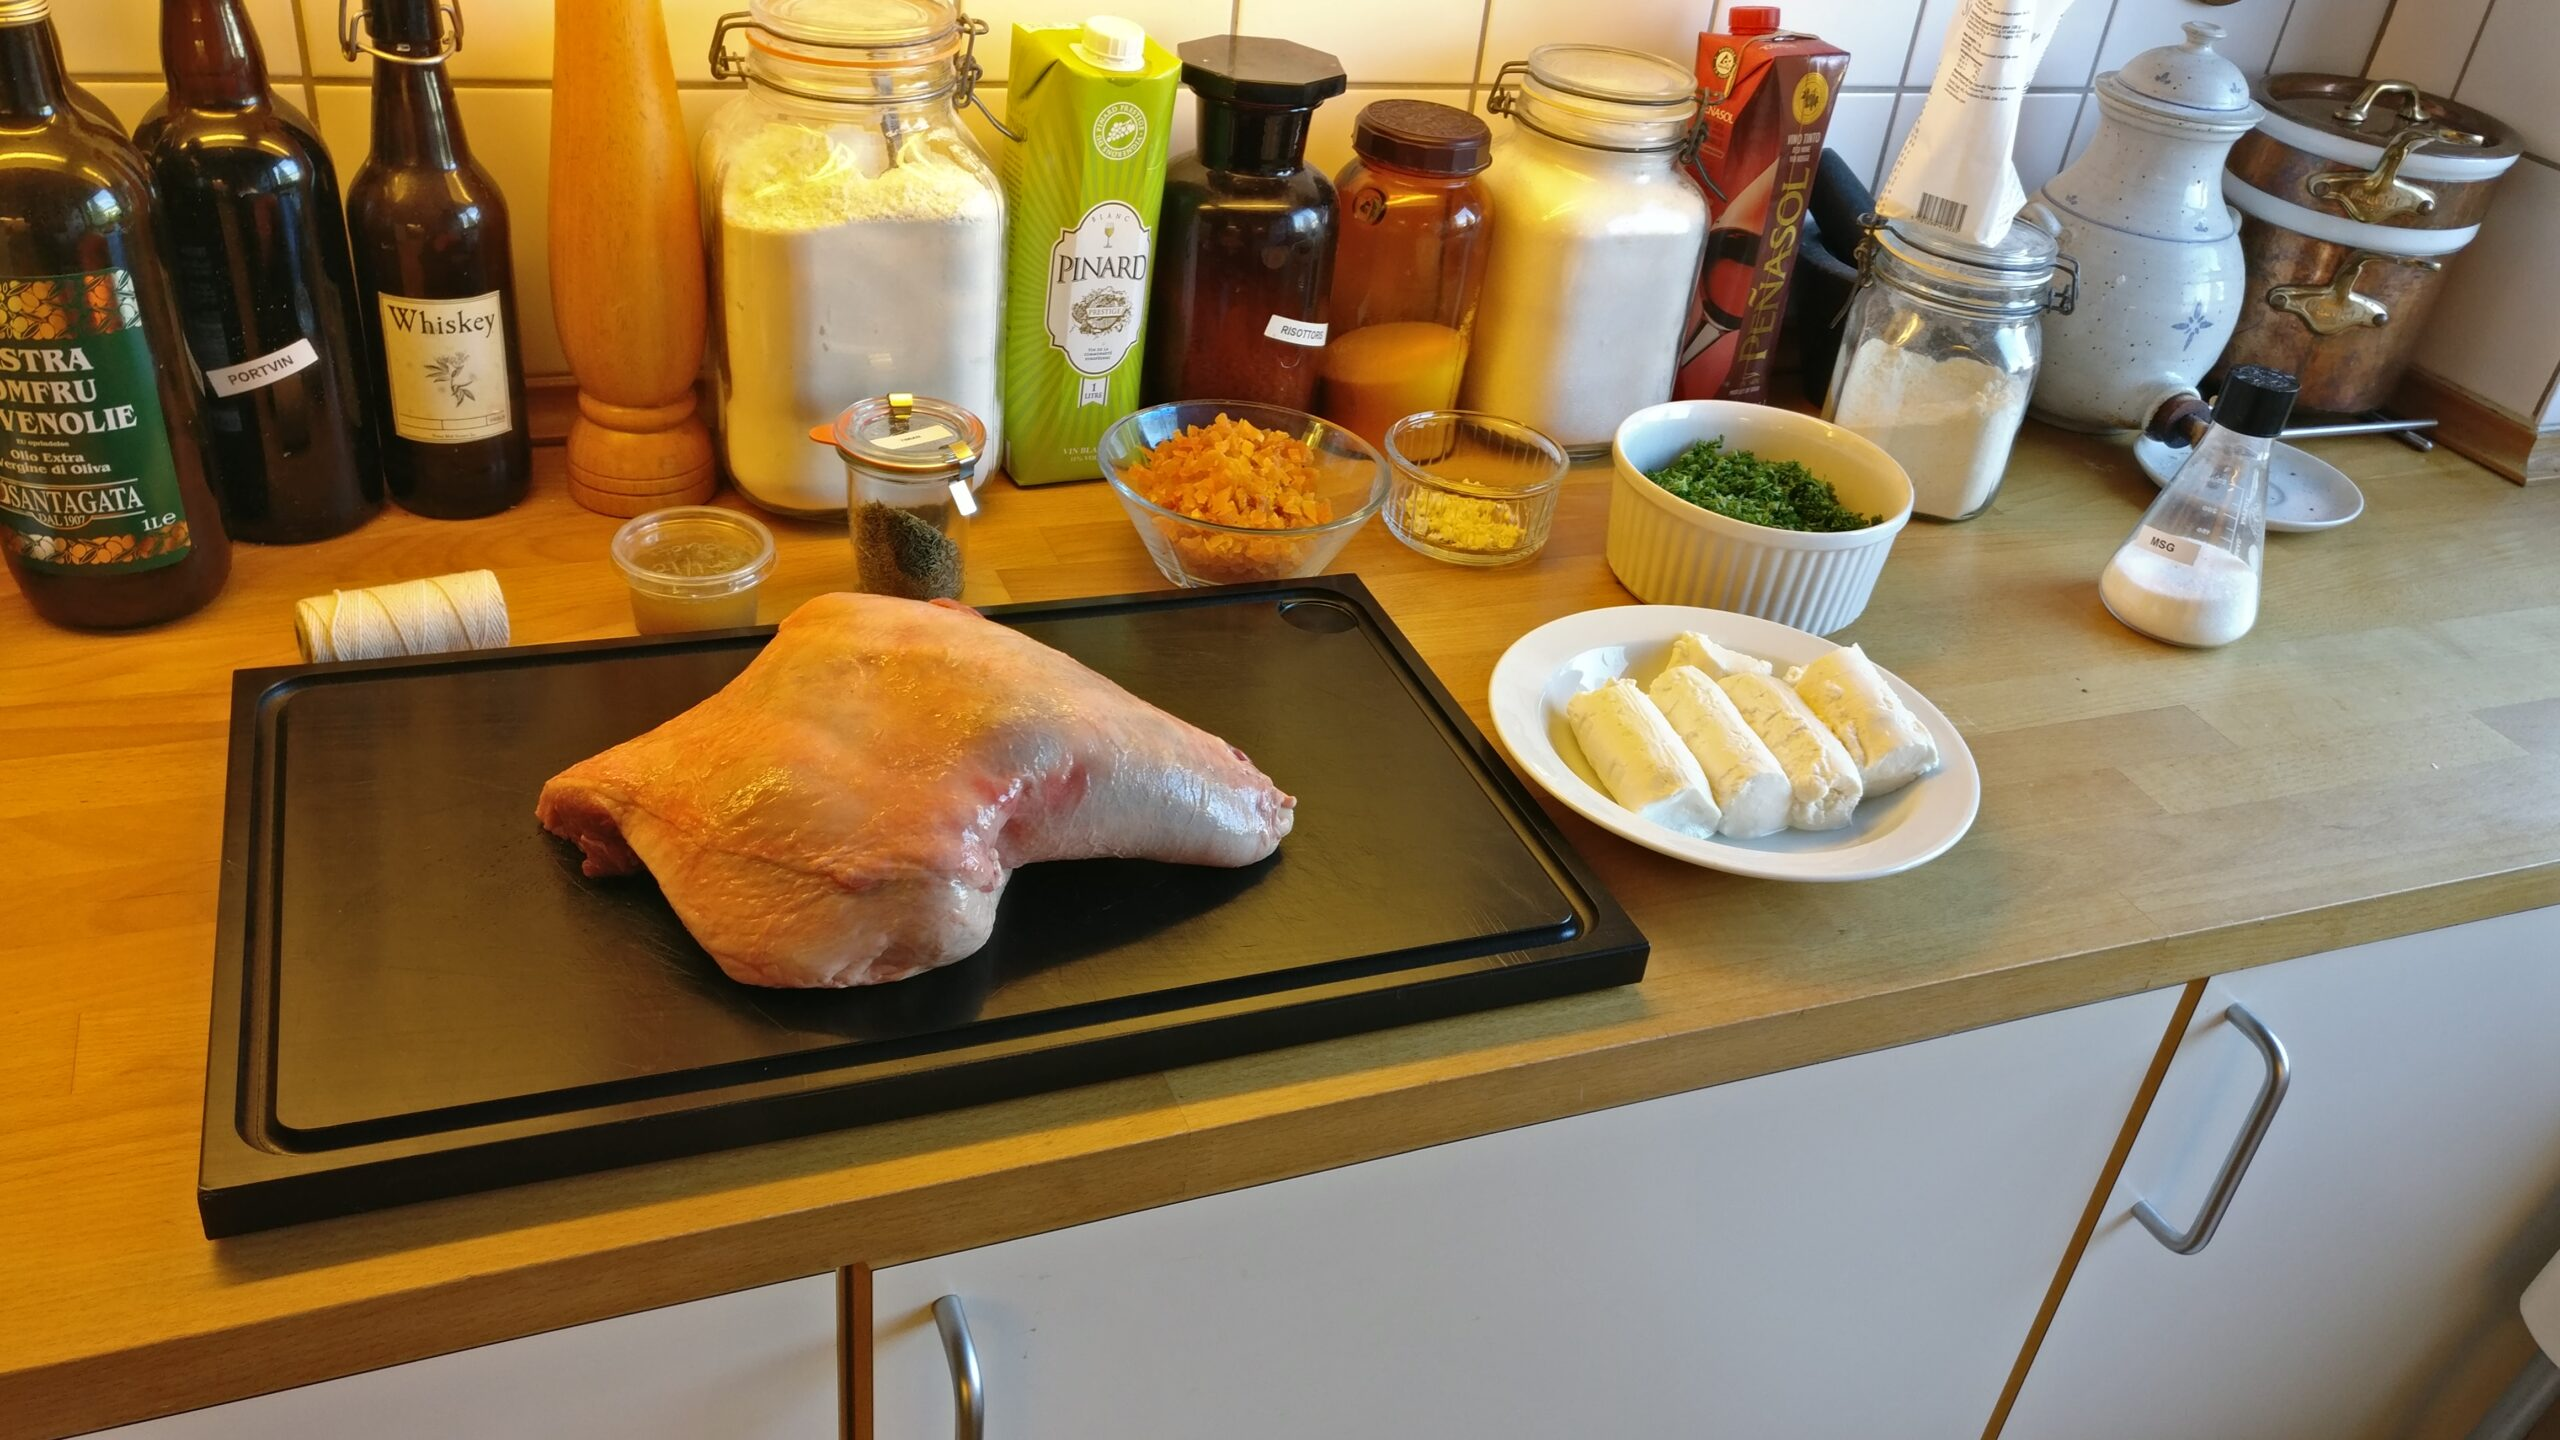
\includegraphics{rmds/images/lam1-scaled.jpg}
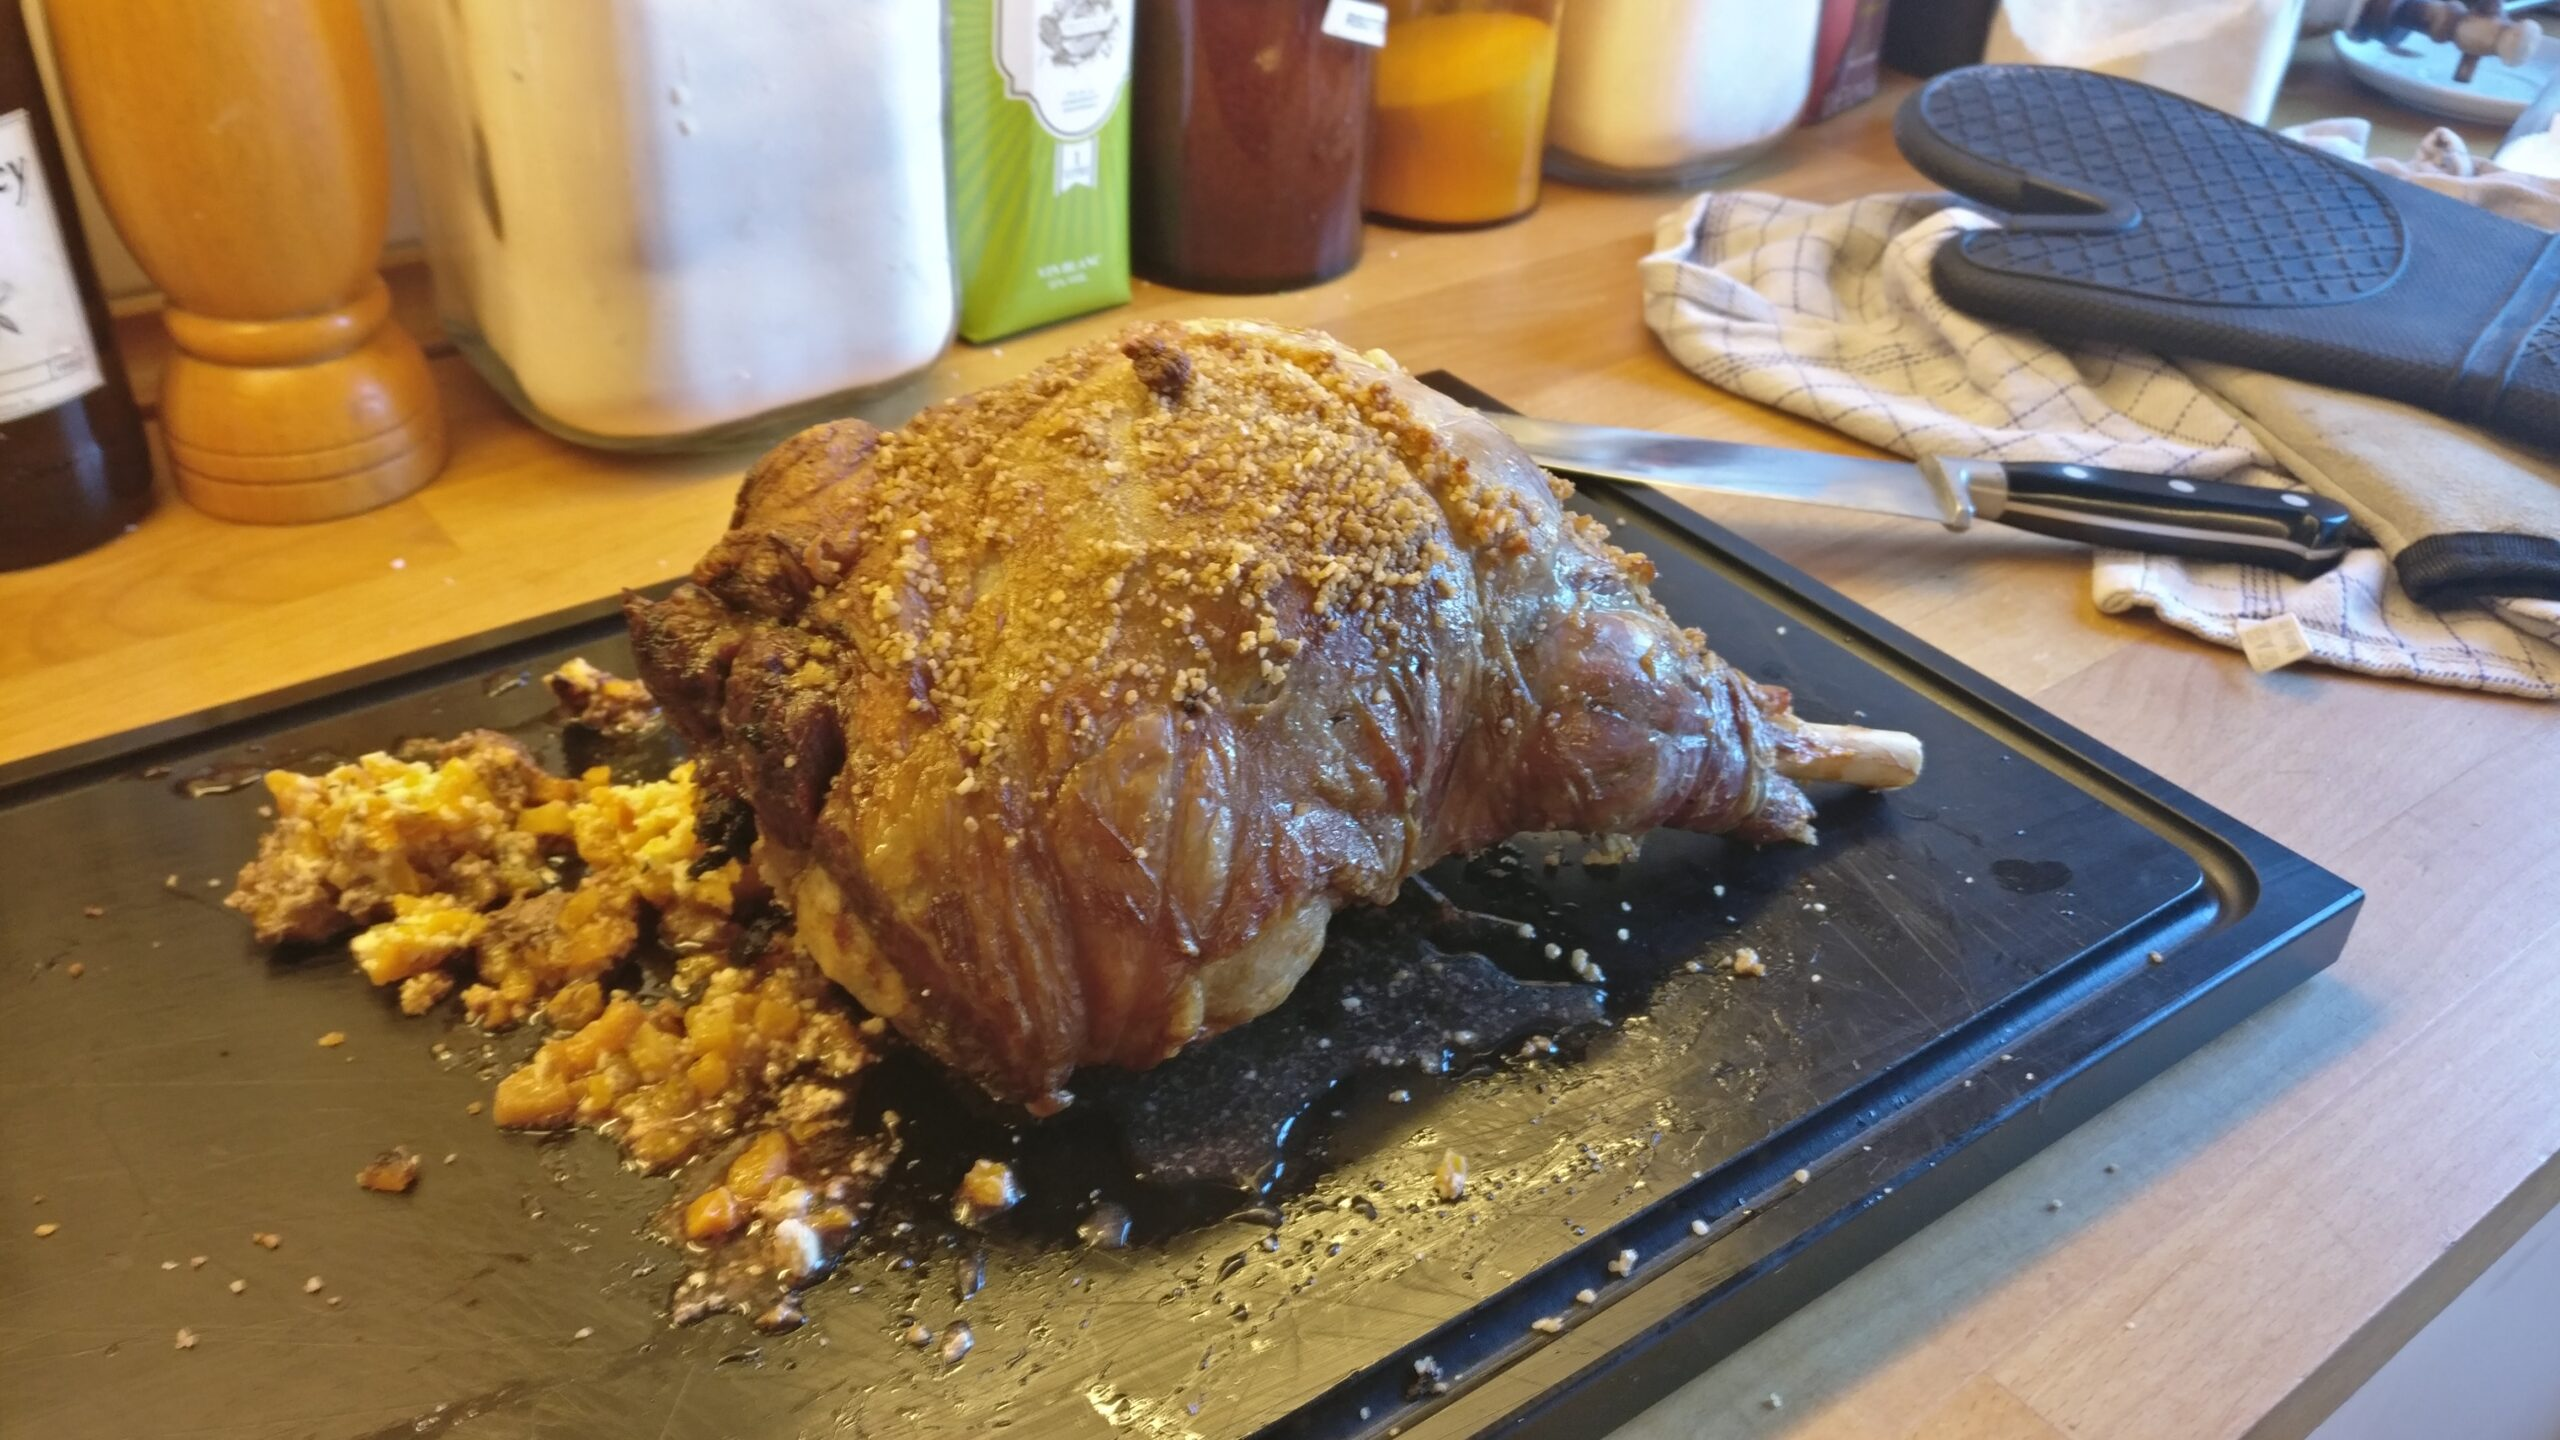
\includegraphics{rmds/images/lam2-scaled.jpg}

Stegesnoren pilles af, og der skæres skiver af køllen. Server dyret oven
på kartoflerne. Man kan godt give en gang bønner eller lidt salat til.

\bookmarksetup{startatroot}

\hypertarget{vildt}{%
\chapter{Vildt}\label{vildt}}

\hypertarget{kanin}{%
\section{Kanin}\label{kanin}}

\hypertarget{forloren-gedegryde.}{%
\subsection{Forloren gedegryde.}\label{forloren-gedegryde.}}

Nej, der er ikke ged i. Men når der er improviseret i køkkenet, er
spørgsmålet ofte: ``Hvad hedder det?''. Det aner jeg ikke, jeg har jo
improviseret. Modspørgsmålet er derfor: ``Hvad har du lyst til at kalde
det?''.

Svaret denne gang var ``Forloren gedegryde''. Og det er jo rigtig nok.
Der er ikke ægte ged i.

\begin{figure}

{\centering 
\includegraphics{rmds/images/DALL-E-notagoat.png}

}

\caption{Not a goat}

\end{figure}

\begin{itemize}
\tightlist
\item
  ½ kanin
\item
  1 spsk sennepspulver
\item
  1 finthakket løg
\item
  4 finthakkede hvidløg
\item
  1 æble (skrællet og i mindre stykker)
\item
  ½ rulle gedeost
\item
  2½ dl piskefløde
\item
  ½ liter kyllingefond/mælk
\item
  Lidt sherry
\item
  Smør og mel
\item
  Salt, peber
\end{itemize}

Kaninen gnubbes med salt, peber og en spsk sennepspulver, og hygger sig
i køleskabet en 5-6 timer. Kaninus brunes i stegegryden, og tages op.
Løgene klares, og hvidløg og æble tilsættes, og får lidt varme. Gryden
koges af med en sjat sherry, og fløde, kyllingefond og/eller mælk
tilsættes. Jeg gav den 2½ dl fløde, der var ikke så meget kyllingefond
tilbage i skabet, så der blev suppleret op med skummetmælk, til det
passede. En ½ rulle gedeost var til overs fra produktionen af
nytårssnacks. Den blev skrællet og dumpet i sovsen også. Kog sovsen
igennem til æblerne er gået i opløsning.

Lad Ninka Ninus vende tilbage til gryden, og lad det simre i ca. 20
minutter. Sovsen jævnes med en melbolle, og smages til med salt, peber
og lidt mere sennepspulver.

Jeg serverede den med ris og ærter. Og der blev spist op.

\bookmarksetup{startatroot}

\hypertarget{pasta}{%
\chapter{Pasta}\label{pasta}}

\hypertarget{carbonara-ala-noma}{%
\section{Carbonara ala noma}\label{carbonara-ala-noma}}

\begin{itemize}
\tightlist
\item
  100 gram pancetta - eller bacon i små tern
\item
  200 gram tør pasta
\item
  25 g røget svampe garum
\item
  4 store æggeblommer
\item
  100 g pecorino Romano fint revet
\item
  salt og peber
\end{itemize}

Bring vand i kog - med salt. Ikke så meget at det smager salt. Men så
det smager som om det har fået noget.

Steg, ved lav varme, baconen. Den må godt stege, men ikke sprøjte. Målet
er at få fedtet ud uden at baconen bliver mørk.

Fjern 3/4 af fedtet og placer det i en stor skål. Steg resten af baconen
til den er sprød. Den, og fedtet føres til separat skål.

I den store skål fra før, tilsættes garum, æggeblommer og pecorino.
Bland godt til en pasta

Kog pastaen til den er lige under al dente. Sigt pastaen i dørslag. Men
gem vandet.

Tilføj lidt af det varme pastavand til skålen og rør voldsomt. Når den
ikke længere er stiv, hældes pastaen i, sammen med friskkværnet peber og
bland godt. Giv evt lidt mere pastavand hvis den er for tør. Smag til
med salt.

Server i skåle med den sprøde bacon ovenpå, mere peber og et solidt drøs
pecorino. Hvis ikke sovsen tykner så sæt den på vandbad (så -
pastagryden?). Men pas på den ikke får for meget varme.

\hypertarget{peberpasta}{%
\section{Peberpasta}\label{peberpasta}}

En Caico e pepe variant

\begin{itemize}
\tightlist
\item
  320 gram pasta
\item
  4 spsk smør (eller oliven olie)
\item
  2 1/4 spsk peber - gerne Triple Lemon Pepper fra Mill \& Mortar
\item
  2½ dl revet parmasan
\item
  hakket persille eller basilikum
\end{itemize}

Kog pastaen til den der er al dente. Dræn, gem kogevand.

Rør pasta sammen med smør i pande eller stor gryde. Tilsæt peber og 2-3
dl kogevand. Rør mere rundt under god varme.

Tag af kogepladen og tilsæt os. Andret med basilikum eller persille.

Server med stegt kylling, godt brød eller lignende.

\hypertarget{misopasta}{%
\section{Misopasta}\label{misopasta}}

\begin{itemize}
\tightlist
\item
  310 gram pasta - linguine eller bucatini
\item
  6 spsk smør
\item
  3 spsk miso (sådan en vejer 18 gram)
\item
  100 gram revet parmasan
\end{itemize}

Bring vand i kog, og kog pastaen.

Imens samler vi smør og miso i en gryde eller lignende - jeg bruger min
sauterpande. Der røres ret grundigt rundt. Tilsæt den næsten færdige
pasta og 2½ dl eller så kogevand fra pastaen. Samt parmasanen. Rør
aggresivt, indtil osten er smeltet og sovsen danner en emulsion.

Bum. Server evt noget kylling i skiver, en grøntsag eller noget.

\hypertarget{mac-n-peas}{%
\section{Mac n Peas}\label{mac-n-peas}}

\begin{itemize}
\tightlist
\item
  600 g frostærter
\item
  310 g makaroni
\item
  50 g smør
\item
  3 fed hvidløg
\item
  60 g parmasan
\end{itemize}

Kog ærter og makeroni Hak hvidløg fint, og lun i smørret på sauterpanden
Overfør de fleste af ærterne til panden, og stavblend sammen med
parmasanen (og salt og peber) De resterende hele ærter, evt også lidt
kogevand, samt makeroni røres sammen med ærtemosen i panden.

Server et par af Faktas (nu 365s) flutes til.

\hypertarget{pasta-al-dante}{%
\section{Pasta al Dante}\label{pasta-al-dante}}

Dante skrev i følge overleveringen sine digte på en plads med udsigtover
byggepladsen hvor Duomoen blev bygget. I følge rygterne havde han en
overmenneskelig hukommelse. En forbipasserende skulle have spurgt ham
hvad der var bedst at spise. Og han svarede prompte ``æg''. Den samme
forbipasserende fandt hm et år senere siddende samme sted, og spurgte
``Med hvad''. Hvortil Dante skulle have svaret, lige så prompte - ``Med
salt''.

Ingredienser

\begin{itemize}
\tightlist
\item
  300 g bucatini
\item
  2 af faktas flutes
\item
  3 fed hvidløg
\item
  Æg
\item
  lidt chiliflager
\end{itemize}

\hypertarget{italiensk-puxf8lseret}{%
\section{Italiensk pølseret}\label{italiensk-puxf8lseret}}

Eller ``Pasta con Salsiccia e Tartufo''

Superenkel ret. Og det er jo altid godt.

En pakke små italienske pølser Trøffelpasta mindst 3 tsk 1½ dl hvidvin
2½ dl fløde 1 stilk frisk rosmarin 1 dl god olivenolie Revet parmasan
Pasta - gerne rigatone

Pil skindet af pølserne, og hak dem. Lad dem simre i en pande med olien
i 5 minutter.

Tilsæt rosmarin, 1 tsk trøffelpasta og hvidvin. Kog alkoholen af, og
tilsæt fløden.

Kog pastaen. Nu er timingen vigtig. Sovsen skal have kogt ind til rette
tykkelse, ca. samtidig med at pastaen er færdig. Man kan snyde og koge
sovsen ind, og så tage den af pladen mens man koger pasta.

Vend pasta og sovs sammen, giv den yderligere 2-3 tsk trøfelpasta og
nogle solide rev parmasan.

Det er min erfaring af pølserne giver tilstrækkeligt salt og peber, men
smag lige til undervejs.

\hypertarget{standard-pastabix}{%
\section{Standard pastabix}\label{standard-pastabix}}

\hypertarget{onepot-pasta}{%
\section{Onepot Pasta}\label{onepot-pasta}}

\hypertarget{putanesca}{%
\section{Putanesca}\label{putanesca}}

også kendt som Luderpasta Ingredienser

\begin{itemize}
\tightlist
\item
  200 g sorte oliven
\item
  2 spsk kapers
\item
  4-5 rensede ansjoser
\item
  3 fed hvidløg
\item
  1-2 peperocini
\item
  1 dåse flåede tomater
\item
  1 spsk revet citronskal
\item
  1 håndfuld persille
\item
  1 smule olivenolie
\item
  320 gram spaghetti
\end{itemize}

Hak det hele fint, hver for sig.

olien varmes op på panden, og hvidløg og peperocini svitses. Hvidløget
må ikke blive brunt. Og peberen er en smagssag.

Tilsæt oliven, kapers og ansjoser. Steg lidt under omrøring

flåede tomater tilsættes.

Lad det simre mens pastaen koges.

Smag sovsen til med slat og peber, lidt sukker og hakket persille samt
citronskal.

Bland pastaen i. juster evt. tykkelsen af sovsen med pastavandet.

\hypertarget{aglio-et-olio}{%
\section{Aglio et olio}\label{aglio-et-olio}}

Ingredienser

\begin{itemize}
\tightlist
\item
  400 g bucatini er passende. Prøv med 410 gram næste gang.
\item
  4 fed hvidløg, finthakket
\item
  4 spsk god olivenolie
\item
  parmasan - 53 gram er for lidt
\item
  hakket persille - en håndfuld.
\item
  Chili - nok bedre med en peperonici eller hvad den nu hedder En enkelt
  tørret chili er passende
\end{itemize}

Hak chili og hvidløg, og lun i olien i sauterpanden. Det går hurtigt, så
det kan godt vente til pastaen er i vandet.

Kog pastaen til den er al dente, Vend pastaen i olien og rør sammen med
parmasan og persille

2 af faktas flutes ting til.

\hypertarget{one-pot-lasagne}{%
\section{One pot lasagne}\label{one-pot-lasagne}}

Vi så store mængder youtubevideoer. Med en eller anden der ikke hedder
Babish, men kalder sig det alligevel. Eller noget.

Ricottaen er pillet ud. 2 klodser moz er fint. En karton pizzasovs, og
en enkelt dåse hakket tomat er også nok. 400 gram hakket ko. Og så kom
jeg i første omgang noget der minder om 15 lasagneplader i - og det var
i overkanten.

originalen:

\begin{itemize}
\tightlist
\item
  10 lasagneplader
\item
  1 spsk oliven olie
\item
  ½ kg spicy italiensk pølse. Men vi bruger hakket kød
\item
  ½ stort løg
\item
  2 fed hvidløg
\item
  1 tsk røde peber flager
\item
  28 oz knuste san marzano tomater. på dåse
\item
  ½ cup varmt vand
\item
  8 oz tomatsovs
\item
  8 oz mozarella
\item
  basilikum. Og sådan
\end{itemize}

https://basicswithbabish.co/basicsepisodes/onepot-pasta

\hypertarget{pasta-med-broccoli}{%
\section{Pasta med broccoli}\label{pasta-med-broccoli}}

\begin{itemize}
\tightlist
\item
  400 gram pasta
\item
  1 stor buket broccoli - eller 2 små, det er sådan de kommer i mit
  supermarked.
\item
  5 hvidløg
\item
  7 ansjosfilleter (i olie)
\item
  Chili/peperoncini eller lign. et mellemstort nip
\item
  olie
\item
  peber
\item
  Revet parmasam
\end{itemize}

Skær broccoli i små buketter, skræl og skær stokken ud i mindre stykker.

Kog broccolien i let saltet vand - til den stadig er relativt fast. Si
vandet fra broccolien.

Sæt pastaen over. 10 gram salt per liter vand.

Hak hvidløg og ansjoser, og steg hvidløgene i olivenolie i en
sasuterpande sammen med chilien i et par minutter. Tilsæt ansjoserne, og
steg videre til fisken er smeltet. Giv det evt lidt pastavand hvis det
bliver tørt.

Smid broccolien i panden, og steg dem med.

Det skal først ske når pastaen er næsten færdig, ellers bliver
broccolien let for smattet.

Smid den al dente pasta i panden, bland, og tilsæt parmasan, smag til
med peber og juster med pastavand.

\hypertarget{gnocchetti}{%
\section{Gnocchetti}\label{gnocchetti}}

Bittesmå gnocchi. Lækkert.

Lige dele pr volumen (sådan ca. der skal måles efter) af tipo-00 og
ricotta, helt den fuldfede i stedet for den fedtreducerede æltes sammen
med ½ tsk salt (hvs det er ca. 250 gram af hver). Hviler på køl, trilles
ud til pølse i ca. blyantstykkelse. Hakkes ud i ca. 1 cm længde. Koges -
de skal have et par minutter efter de har fundet op til overfladen.

Serveres med noget tomatsovs. Eller bare god parmasan. Der skal en sjat
mere til for at det rækker til os to.

\hypertarget{sticky-honey-garlic-sausage-pasta-skillet}{%
\section{Sticky Honey Garlic Sausage Pasta
Skillet}\label{sticky-honey-garlic-sausage-pasta-skillet}}

Ingredients: * 1 lb Italian sausage (or your choice of sausage) * 12 oz
pasta (penne, rigatoni, or your preferred type) * 2 tbsp olive oil * 4
cloves garlic, minced * 1/4 cup honey * 2 tbsp soy sauce * 1 tbsp Dijon
mustard (optional) * 1/2 tsp red pepper flakes (optional, for a spicy
kick) * Salt and pepper, to taste * Fresh parsley or basil, chopped, for
garnish * Grated Parmesan cheese (optional, for topping)

Og her kan der skrues en del op for chilipeberen.

Instructions: Cook the pasta: In a large pot, bring salted water to a
boil. Add the pasta and cook according to package instructions until al
dente. Drain and set aside. Cook the sausage: While the pasta is
cooking, heat olive oil in a large skillet over medium heat. Add the
sausage (remove the casing if using link sausage) and cook until
browned, breaking it up into small pieces as it cooks. This should take
about 5-7 minutes. Make the sauce: Add the minced garlic to the skillet
with the sausage and cook for 1-3 minutes, until fragrant. Stir in the
honey, soy sauce, Dijon mustard (if using), and red pepper flakes. Allow
the mixture to simmer for 4-6 minutes until the sauce thickens slightly.
Combine pasta and sauce: Add the cooked pasta to the skillet, tossing to
coat the pasta in the sticky sauce. Let everything cook together for
another 2-3 minutes, allowing the flavors to meld. Season: Taste and
season with salt and pepper as needed. Serve: Garnish with fresh parsley
or basil, and top with grated Parmesan cheese if desired. Serve warm and
enjoy your sticky honey garlic sausage pasta skillet!

\hypertarget{pasta-med-broccoli-1}{%
\subsection{Pasta med broccoli}\label{pasta-med-broccoli-1}}

Lad os bare være ærlige - den er nappet fra James Price.

\begin{itemize}
\tightlist
\item
  400 gram pasta
\item
  1 stor buket broccoli - eller 2 små, det er sådan de kommer i mit
  supermarked.
\item
  5 hvidløg
\item
  7 ansjosfilleter (i olie)
\item
  Chili/peperoncini eller lign. et mellemstort nip
\item
  olie
\item
  peber
\item
  Revet parmasam
\end{itemize}

Skær broccoli i små buketter, skræl og skær stokken ud i mindre stykker.

Kog broccolien i let saltet vand - til den stadig er relativt fast. Si
vandet fra broccolien.

Sæt pastaen over. 10 gram salt per liter vand.

Hak hvidløg og ansjoser, og steg hvidløgene i olivenolie i en
sasuterpande sammen med chilien i et par minutter. Tilsæt ansjoserne, og
steg videre til fisken er smeltet. Giv det evt lidt pastavand hvis det
bliver tørt.

Smid broccolien i panden, og steg dem med.

Det skal først ske når pastaen er næsten færdig, ellers bliver
broccolien let for smattet.

Smid den al dente pasta i panden, bland, og tilsæt parmasan, smag til
med peber og juster med pastavand.

\hypertarget{one-pan-sweet-tangy-bbq-sausage-rice}{%
\subsection{One-Pan Sweet \& Tangy BBQ Sausage
Rice}\label{one-pan-sweet-tangy-bbq-sausage-rice}}

NB ikke pasta. Men\ldots{}

\begin{itemize}
\item
  450 g røget pølse - skåret i skiver
\item
  300 g ris
\item
  1 peberfrugt - i tern
\item
  1 løg - i tern
\item
  2 fed hvidløg - hakket
\item
  ½ l kyllingefond
\item
  1½ dl BBQ-sovs
\item
  olivenolie
\item
  1 tsk røget paprika

  ½ tsp garlic powder

  ½ tsp onion powder

  ¼ tsp black pepper

  Pinch of red pepper flakes (optional, for heat)
\end{itemize}

(Optional garnish: Chopped parsley or green onions)

Brun pølseskiverne i olien i 3-4 minutter. Tag dem fra. Sauter
grønsagerne i ca. 3 minutter Rør hvidløg i og giv dem lidt varme.

\begin{enumerate}
\def\labelenumi{\arabic{enumi}.}
\setcounter{enumi}{2}
\tightlist
\item
  Add Rice \& Seasonings
\end{enumerate}

Pour in rice, smoked paprika, garlic powder, onion powder, black pepper,
and red pepper flakes. Stir to coat.

\begin{enumerate}
\def\labelenumi{\arabic{enumi}.}
\setcounter{enumi}{3}
\tightlist
\item
  Simmer to Perfection
\end{enumerate}

Add chicken broth and BBQ sauce, then return sausage to the pan. Bring
to a boil, then reduce heat to low, cover, and simmer 18-20 minutes
until rice is tender.

\begin{enumerate}
\def\labelenumi{\arabic{enumi}.}
\setcounter{enumi}{4}
\tightlist
\item
  Serve \& Enjoy!
\end{enumerate}

Fluff rice with a fork, drizzle with extra BBQ sauce, and garnish with
parsley or green onions.

\hypertarget{one-pot-lasagne-1}{%
\section{One Pot lasagne}\label{one-pot-lasagne-1}}

Vi så store mængder youtubevideoer. Med en eller anden der ikke hedder
babish, men kalder sig det alligevel.

Ricottaen er pillet ud. 2 klodser moz er fint. En karton pizzasovs, og
en enkelt dåse hakket tomat er også nok. 400 gram hakket ko. Og så kom
jeg i første omgang noget der minder om 15 lasagneplader i - og det var
i overkanten. https://basicswithbabish.co/basicsepisodes/onepot-pasta

originalen: * 10 lasagneplader * 1 spsk oliven olie * ½ kg spicy
italiensk pølse. Men vi bruger hakket kød * ½ stort løg * 2 fed hvidløg
* 1 tsk røde peber flager * 28 oz knuste san marzano tomater. på dåse *
½ cupå varmt vand * 8 oz tomatsovs * 8 oz mozarella * basilikum. Og
sådan

https://basicswithbabish.co/basicsepisodes/onepot-pasta

\hypertarget{makaronipie}{%
\section{Makaronipie}\label{makaronipie}}

En af Metas opskrifter. 75 g makaroni koges i

4 dl mælk

3 æggeblommer røres med

75 g sukker. Deri kommes

3 dl mælk, 75 g smeltet margarine og de piskede hvider.

Makeroni vendes i og bages ca 1 time.

Hvor længe der skal bages skriver Meta ikke noget om.

\hypertarget{pasta-med-knuste-uxe6rter}{%
\section{Pasta med knuste ærter}\label{pasta-med-knuste-uxe6rter}}

Inspireret af Hugh-Fearnley-Whittingstall

\begin{itemize}
\tightlist
\item
  600 g frosne ærter
\item
  350 g pasta - det fungerer bedst med de små typer.
\item
  50 g smør
\item
  2 fed hvidløg - finthakket
\item
  25 g revet parmasan
\item
  Salt og peber
\end{itemize}

Ærterne hældes i gryde og dækkes med vand. Bring det i kog, og kog til
ærterne er møre. Der er mere smag i friske ærter, men de skal koge
længere.

Heromkring koges pastaen. Det skal måske justeres lidt afhængig af
pastatypen, og hvor hurtigt man forventer at de næste trin kan gøres.

Smelt smørret i en mindre gryde. Lav varme, det skal ikke brune. Steg
hvidløget i smørret - hvidløget må heller ikke tage farve.

Gem et par kopper af vandet fra ærterne, og hæld resten fra. Smid
halvdelen af ærterne i gryden med ca. 1 dl af kogevandet og osten.
Blendt med stavblender til pureen er glat. Juster evt med lidt mere
vand. Hæld resten af ærterne i gryden og smag til med salt og peber.

Hæld vandet fra pastaen, og vend den med ærtepureen. Giv den et strøg
parmasan eller tre, og server med brød.

\hypertarget{en-grydes-pasta}{%
\section{En grydes pasta}\label{en-grydes-pasta}}

Jeg har en standardopskrift på pasta når det skal gå hurtigt.
Kobber-sauterpanden kommer i brug. Den store gryde bruges til pastaen.
Og så er der en skål og et piskeris, og en tang, og en pastaske der også
bliver beskidt. Og det er før vi får maden på tallerkenerne.

Det er hurtigt, det er (som regel) godt, og det er godt når det er mig
der står for maden, og arbejdsugen (igen) har sneget sig op på 43 timer.

Men det er også mig der står for opvasken (grrrr). Så hvis nu man kunne
minimere opvasken.

Martha Stewart har en opskrift på pasta i en enkelt gryde. Og det er
hurtigt. Med danske mål, til fire personer:

\begin{itemize}
\tightlist
\item
  350 gram pasta
\item
  350 gram cherrytomater, halveret
\item
  1 løg, skåret i tynde skiver
\item
  4 fed hvidløg, skåret i tynde skiver
\item
  ½ tsk basilikum
\item
  2 spsk olivenolie
\item
  Salt, peber
\item
  1,1 l vand
\end{itemize}

Det hele hældes i en gryde, bringes i kog ved høj varme. Der røres
hyppigt, indtil pastaen er al dente, og næsten alt vandet er kogt væk.
Ca. 9 minutter.

Jeg tror ikke helt på de 9 minutter. Uanset hvad de skriver på pakkerne,
tager det altid længere. Men det skal ikke afholde mig fra at prøve
opskriften ved lejlighed.

I aften står den dog på fritter og fiskefileter. Vi skal have ryddet ud
i fryseren, og der skal ikke eksperimenteres med nye opskrifter når jeg
samtidig skal tage opvasken fra i søndags.

\hypertarget{alternativ-pasta-carbonara}{%
\section{Alternativ pasta carbonara}\label{alternativ-pasta-carbonara}}

Kog pastaen. Lav en ægte sovs af to æg, 1½ dl fløde, 50 gram friskrevet
parmasan, salt og peber. Også kendt som, hæld det hele i en kasserolle
og varm forsigtigt op under konstant omrøring. Steg bacon, løg, hvidløg
og rosmarin på en pande (hvidløget skal først med til sidst). Saml alle
delene. Suppler gerne med grønne asparges eller svampe.

\hypertarget{standard-pastaopskrift}{%
\section{standard pastaopskrift}\label{standard-pastaopskrift}}

Det er ulvetimen. Det skal gå hurtigt. Arbejdet har været hæsligt og
trukket ud igen. Vi har godt nok ikke børn der skal hentes og fodres,
men derfor skal aftensmaden klares i en ruf alligevel.

Standardopskriften i de situationer er:

Ingredienser:

½ kg frisk pasta 1/4~l madlavningsfløde, eller flødesubstitut. Evt.
rigtig fløde hvis det skal være godt. 2 store håndfulde friskrevet
parmasan 250-300 g lakserester, hakket ko, chorizo, kyllingestykker
eller andet protein Salt, peber, evt. basilikum, timian, hvidløg eller
hvad der nu passer. Og olivenolie til at stege.

Fremgangsmåde:

Steg dyret på stor, dyb pande (jeg har en kobber sauterpande. Den er
dyr, men den er god) i olien sammen med krydderierne. Kog imens pastaen.
Husk salt. Rør ost og flødetingen sammen. Husk, at hvis du er syndig og
det er rigtig fløde, så skal der ret meget salt i. Når pastaen er kogt,
løftes den over i panden til dyret, og der blandes godt. Hæld oste/fløde
blandingen over, ~og bland endnu mere. Og her er det hemmelige trick:
Hæld en kop eller to af kogevandet fra pastaen i. Det får sovsen til at
creme, og gør det hele ekstra lækkert! Server med brød og/eller salat.
Og gerne lidt ekstra parmasanost.

\bookmarksetup{startatroot}

\hypertarget{det-gruxf8nne}{%
\chapter{Det grønne}\label{det-gruxf8nne}}

\hypertarget{svampe-og-safran-risotto}{%
\section{Svampe og safran risotto}\label{svampe-og-safran-risotto}}

Generelt bruger vi 4 dl risotto ris når der laves risotto. 120 gram
passer også fint i denne opskrift.

\begin{itemize}
\tightlist
\item
  25 gram røget svampe garum - eller svampe bouillon
\item
  200 gram svampe - skåret i skiver
\item
  15 gram olivenolie
\item
  15 gram smør
\item
  1 lille løg
\item
  120 gram arborio ris
\item
  10-15 tråde saffran
\item
  600 ml vand
\item
  2 håndfulde revet parmasanost
\end{itemize}

Karameliser svampene i olie. Tilsæt smør og 5 gram garum.

Klar løg i olie Tilføj ris, lad dem blive dækket i olie og giv dem lidt
varme.

Bland resten af garumen og vandet, hæld 400 ml over risene, og tilsæt
også safronen.

Rør konstant til væsken er absorberet. Tilføj resten af væsken,
undervejs - til risen er færidg.

Rør en håndfuld parmasan i - tilføj lidt mere væske, og resten af osten.
Smag til og juster konsistens med væsken.

Tag af varmen, rør svampene i, giv den lidt persille eller lignende
grønt på toppen, og server.

\hypertarget{chachouka}{%
\section{chachouka}\label{chachouka}}

\begin{itemize}
\tightlist
\item
  5 peberfrugter (men det afhænger selvfølgelig af størrelsen) er
  passende.
\item
  6 æg er fint.
\item
  løg
\item
  spidskommen
\item
  paprika (lad nu være med at komme det i fra starten)
\item
  safran
\item
  en dåse hakkede tomater
\item
  salt og peber
\item
  Hvidløg
\end{itemize}

\hypertarget{dahl}{%
\section{Dahl}\label{dahl}}

\begin{itemize}
\tightlist
\item
  210 gram røde linser
\item
  2 spsk revet ingefær
\item
  4 finthakkede hvidløg
\item
  3 tsk karry (medium stærk)
\item
  1 spsk spidskommen
\item
  0,50 spsk stødt koriander
\item
  0,50 tsk stødt kardemomme
\item
  0,50 tsk chiliflager
\item
  6 dl grøntsagsbouillon
\item
  200 g røde linser
\item
  2 dåser hakkede tomater
\item
  2 spsk olivenolie
\end{itemize}

\hypertarget{suxf8ren-davidsens-tomatsuppe}{%
\section{Søren Davidsens
Tomatsuppe}\label{suxf8ren-davidsens-tomatsuppe}}

Som egentlig er fra The Guardian. Men så dør referencen til What We do
in the shadows\ldots{}

Suppen:

\begin{itemize}
\tightlist
\item
  2 auberginer (hvis de er små. 550 gram)
\item
  350 gram cherry tomater
\item
  2 store røde chilier
\item
  100 ml olivenolie
\item
  2½ spsk tomatpasta
\item
  salt og peber
\item
  1 liter kyllinge fond
\item
  1 spsk lemon juice
\item
  Brød croutoner.
\item
  Frisk oregano og persille. Man kan godt klare sig med frossen
  persille.
\end{itemize}

Aiolien

\begin{itemize}
\tightlist
\item
  5 fed hvidløg - finthakket (meget)
\item
  8 ansjoser (fileter) - finthakket (meget)
\item
  90 ml olivenolie
\item
  50 ml solsikkeolie
\item
  1 æggeblomme
\item
  1 spsk lemon juice
\end{itemize}

Hæld hvidløg, ansjoser og olivenolie i en gryde. Det er stærkt fristende
at tage en lille kasserolle. Brug i stedet en der er stor nok til den
samlede mængde suppe, det sparer på opvasken.

Lad det simre ved middel varme i 12 minutter. Pas på at hvidløgene ikke
brænder. Tag af varmen, og flyt 60 gram af blandingen over i en beholder
- tilsæt solsikkeolien.

Lad det nu få samme temperatur som juice og æggeblommen.

Skyl tomaterne, flæk chilierne og fjern det hvide og frøene. Hak
chilierne groft. Skyl auberginerne. Skræl dem i striber - tænk zebra.
Men sørg for at den skræl der er tilbage på auberginerne er ret tynd -
det kan være lidt træls at tygge i ellers. Skær dem ud i 3 cm tykke
skiver. Vend grøntsagerne i olien, giv det en tsk salt, og rigeligt med
peber. Og så skal det i ovnen i en lille bradepande ved 210 grader
varmluft i 45 minutter. Vend det hele ca. halvvejs.

Resten af hvidløg/ansjos/olie blandingen fra før får nu varme, og
tomatpureen/pastaen varmes igennem i ca. 4 minutter. Tilsæt fond og
juice. Og en kvar tsk salt. Lad det simre i 15 minutter ved middel
varme.

Nu rører vi æggeblommen sammen med 1/8 tsk salt og juicen. Og rører
derefter en mayonaise med den olie vi tog fra tidligere (og blandede med
mere olie). Lad dig ikke friste af den oprindelige opskrift der
foreskriver en foodprocessor. Håndkraft og et gammeldags piskeris fra
Raadvad er vejen frem her!

De stegte grøntsager fordeles i fire skåle, suppen fordeles i samme
skåle. Kroutoner drysses over, en solid klat aioli oven i. Drys med
krydderurterne og et par vrid peber. Server straks.

Eller placer grøntsagerne i et lille fad, og sæt gryden på bordet sammen
med kroutoner og aioli, hvis det ikke behøver at være meget fornemt og
fancy.

\bookmarksetup{startatroot}

\hypertarget{snyde-morgenmads-tuxe6rte}{%
\chapter{Snyde-morgenmads-tærte}\label{snyde-morgenmads-tuxe6rte}}

Eller - til frokost. Den går også fint til aftensmaden.

\begin{itemize}
\tightlist
\item
  200 gram svampe
\item
  200 gram frisk spinat- renset
\item
  275 gram butterdej fra supermarkedet
\item
  1 spsk mascarpone
\item
  1 håndfuld friskrevet parmasan
\item
  1 spsk røget svampe garum
\item
  4 æg
\end{itemize}

Tænd ovnen på 180 grader c. Flå svampene fra hinanden og læg dem i en
bradepande med bagepapir. Sæt den i ovnen mens den forvarmer, så de
tørres en smule.

Spinat i skål, overhæld med kogende vand. Sigt vandet fra så snart
spinaten har været dækket med vand.

Tryk vandet af spinaten - så snart det er koldt nok til at du kan
håndtere det. Nej, der er ikke meget tilbage.

Når svampene har været i ovnen ca. 10 minutter, tages de ud og hældes i
skål. Tilføj garummen og slyng svampene rundt i det.

Tilføj spinaten, hvor du trækker bladene ud fra den klump du fik ud af
at trykke vandet fra.

balnd godt med hænderne. Tilføj mascarpone og ost og fold det sammen.

Tag butterdejen fra køleskabet og placer det på en bageplade. Bare lad
bagepapiret fra butterdejen blive på. Smid svampe/spinat/oste blandingen
på butterdejen. Brug en ske til at lave fire små fordybning. Slå de fire
æg ud i fordybningerne.

Fold hjørnerne af butterdejen ind mod midten af tærten. Trim evt lidt af
bagepapiret af med en saks. Pensl dejen med et pisket æg eller mælk, og
bag i 20 minutter.

\hypertarget{dahl-1}{%
\section{Dahl}\label{dahl-1}}

Eller Daal. En indisk klassiker. Linser lyder utroligt kedeligt og
trist, ja nærmest vegansk. Og det kan det også godt være. I min udgave
kommer der dog pølser i. For vegetarer er noget vi tilbereder og spiser
her i huset.

2 spsk olivenolie 4 finthakkede hvidløg 2 tsk stødt ingefær 3 tsk karry
1 spsk stødt spidskommen ½ spsk stødt koriander ½ tsk stødt kardemomme ½
tsk chiliflager (eller bare chilipulver) 6 dl grøntsagsbouillon. (6 dl
vand og en bouillonterning) 200 gram røde linser 2 dåser hakkede tomater
1 chorizopølse

Varm olien op i en stor gryde - gerne af støbejern - ved middel varme.
Tilsæt hvidløg og rør rundt i 1 minut. Pas på det ikke bliver brunt.
Tilsæt krydderierne og lad dem stege med et minuts tid.

Skyl linserne i en sigte - eller et dørslag hvis huller i det er små
nok, og tilsæt dem til gryden, sammen med resten af ingredienserne -
undtagen pølsen.

Lad det simre under låg i 45 minutter.

Pil skindet af pølsen og skær den i mundrette bidder. Lad den koge med
de sidste 10 minutter. Lidt afhængig af hvor stærkt den er krydret. Og
hvor krydret du vil have din dahl. Smag til med slat og peber.

Og så bør man selvfølgelig spise den med raita (det indiske svar på
tzatziki) og hjemmebagte naanbrød.

Det bliver nu oftere bare med ris.

\hypertarget{glaserede-guleruxf8dder}{%
\section{Glaserede gulerødder}\label{glaserede-guleruxf8dder}}

Hyppigt frembragt i køkkenet. For vi skal have nogen grønsager, og
skamkogte gulerødder fik vi nok af som børn. Men det bliver hurtigt for
kedeligt hvis det bare er gulerødder vendt i honning. Derfor:

1 kg gulerødder 8 spsk smør 1 dl bourbon eller whiskey 1½ dl brun
sukker. Farin eller muscovado. ½ tsk salt 1/4 tsk sort peber 1/4 tsk
cayenne peber Skræl gulerødderne, og skær dem i skiver. Steg dem på
meget varm pande i et minuts tid i 1 spsk smør. Gerne af to omgange,
afhængig af hvor stor din pande er. Tag gulerødderne af panden, og hæld
whiskey på. Pas på, panden er varm, så det kan godt give ret kraftige
alkoholtåger i køkkenet. Lad det koge et halvt minuts tid. Sænk varmen
og tilsæt resten af smørret. Tilsæt sukker, og lad det smelte ind i
smørret. Nu kommer gulerødderne tilbage på panden og røres godt ind i
sovsen. Når det hele bobler, får det lov at hygge sig 5-6 minutter under
låg. Smag til med salt, peber og cayennepeber. Lad det koge - uden låg -
5-7 minutter ekstra. Eller til du synes at glaseringen har den tykkelse
du godt vil have.

\hypertarget{guleruxf8dder-med-ingefuxe6r}{%
\section{Gulerødder med ingefær}\label{guleruxf8dder-med-ingefuxe6r}}

Gulerødder er sundt. Og vi spiser for få grøntsager. Så:

\begin{itemize}
\tightlist
\item
  5-6 gulerødder - afhængig af sult og størrelse.
\item
  En stump frisk ingefær
\item
  1 økocitron
\item
  Salt, peber og olivenolie
\end{itemize}

Skræl gulerødderne, og stiml dem med skrælleren, så du får en lang, flad
strimmel. Fortsæt til der ikke er mere gulerod tilbage. Der skulle nu
være en bunke tynde gulerodsstrimler op køkkenbordet.

Riv lidt frisk ingefær. 5-6 riv afhængig af hvor godt du kan lide
ingefær. Pres citronen.

Varm olivenolien op, steg gulerodsstrimlerne et halvt minuts tid under
omrøring.

Tilsæt ingefær og citronsaft. Og giv den et par riv af citronskallen i
tilgift. Steg videre ca 3 minutter. Smag til med salt og peber. Husk,
grøntsager behøver ikke været gennemkogte - der må godt være lidt bid i
dem.

\hypertarget{pestokartofler}{%
\section{Pestokartofler}\label{pestokartofler}}

En slags pesto i hvert fald.

Svigerinden gør ikke så meget i madlavning (den ene af dem - den anden
gør). Men når hun gør, er det faktisk slet ikke så ringe endda. På
jydsk, hvilket er passende.

Til den yngste af de jydske yndlingsniecers fødselsdag havde hun lavet
nogle pestokartofler der fik mig til at spørge efter opskriften. Det er
ikke en traditionel italiensk pesto, der laves på pinjekerner, men
stadig pesto.

\begin{itemize}
\tightlist
\item
  75 g ristede mandler (giv dem en tur på panden. De skal ikke smuttes)
\item
  1 kg kartofler
\item
  2 dl olivenolie
\item
  1 potte basilikum
\item
  75 g parmesanost (riv den selv. Forrevet parmasan lugter af bræk)
\item
  2 fed hvidløg
\item
  salt og peber
\end{itemize}

Smid alt andet end kartoflerne i blenderen og blend til det er en fin
ensartet masse.

Skræl kartoflerne, skær dem i både, og vend dem i pestoen.

Bag kartoflerne ved 200 grader i 40 minutter. Tada!

\hypertarget{kartoffelkuber}{%
\section{Kartoffelkuber}\label{kartoffelkuber}}

Lyder mere fantastisk end det er.

På den anden side ser det faktisk ok ud, og smager godt. Så mit
forbehold handler vel mest om at det er superenkelt.

En bagekartoffel skæres ud i tern, 4-5 cm på hver kant. Det her er noget
der bør laves i kombination med noget kartoffelmos, pure,~ suppe eller
andet. For der er et enormt spild.

Vend kartoflerne i neutral olie, med salt og peber. Ham der gav mit
tippet til det her hælder karry i, selv har jeg brugt paprika. Det gør
ingen forskel efter min mening, al smagen i krydderiet bliver brændt af
alligevel.

Varm ovnen op til 230 grader, hæld kartoflerne i et fad, og bag dem i 30
minutter.

Skru varmen ned til 150 grader, og bag videre i 10-15 minutter.

Vupti!

\hypertarget{ruxf8dluxf8gsalat}{%
\section{Rødløgsalat}\label{ruxf8dluxf8gsalat}}

Man kan ofte have behov for en hurtig lille side ting til maden. Her en
superenkel lille ting.

Rødløg - snittet i tynde ringe. Vendt med hakket persille og sumak

Jeg aner ikke hvad det hedder, men det er ret godt, gerne til stegt kød.
Og oplevet i Grækenland, uden at jeg ved noget om hvor græsk det
egentlig er.

\hypertarget{tomatsalat}{%
\section{Tomatsalat}\label{tomatsalat}}

Efter en opskrift svigermor har fundet et eller andet sted.

\begin{itemize}
\tightlist
\item
  1 kg små tomater. Gerne nogle orange imellem.
\item
  4 spsk groft salt
\item
  1 bundt hakket basilikum. Eller koriander. Eller en blanding.
\item
  3 fed hvidløg. Finthakket.
\item
  1 spsk oregano
\item
  5 spsk god balsamico eddike
\item
  1 dl olivenolie
\item
  1 tsk sukker
\item
  Salt og peber (men nok mest peber)
\end{itemize}

Skær tomaterne i grove stykker. Bruger du forskellige tomater, så har de
formentlig forskelig størrelse, og så skærer du dem så de har ca. samme
størrelse. Brug gerne de små cherry tomater, san marzane (eller hvad de
nu hedder), små blommetomater.

Vend tomaterne med salt, og lad dem stå i et dørslag og dryppe af i 1½
time.

Krydderurter, hvidløg olie og eddike, sukker og peber blandes til en
dressing. Når tomaterne har trukket samles tomater og marinade i en
skål, og træk et par timer. Smag til med salt. Og server.

\hypertarget{kuxe5lrabisovs}{%
\section{Kålrabisovs}\label{kuxe5lrabisovs}}

Hvad stiller man op med sådan en fætter?

Skær et par kålrabier i små tern. Snit et par hvidløg fint. Smid begge
dele i en tykbundet kasserolle - uden fedtstof, for de skal ristes let,
uden at hvidløget tager farve! Når de er ved at være møre, men stadig
har godt bid, tilsættes fløde og ret store mængder finthakket persille.
Kog til fløden tykner lidt. Smag til med salt og peber. God til lam.

\hypertarget{kartoffelgratin}{%
\section{Kartoffelgratin}\label{kartoffelgratin}}

Fra house of small wonders - skal nok modificeres før publikation

En del endda. Prøv at starte med at gøre noget ved kartoffelsorten.

20 g smør

1 kg kartofler, skrællet og i mindre, mundrette stykker

2 fed hvidløg hakket

420 ml mælk

420 ml fløde

1 tsk salt

½ tsk stødt muskat

1/4 tsk sort peber (stødt)

1/4 tsk cumin

70 g revet emmentaler

40 gram revet parmasan

varm ovnen op til 180 grader

smelt smør i gryde, tilføj kartofler og hvidløg og rør rundt til
kartoflerne er dækket af smør

tilføj mælk, fløde, salt og krydderier, bring i kog og lad simre til
kartoflerne er møre.

Hæld blandingen i form, drys osten over, og bag i 20-25 minutter, til
overfladen er gylden. Drys gerne med persille.

\hypertarget{buxf8nner}{%
\section{Bønner}\label{buxf8nner}}

Vi gør ikke så meget i bønner. Altså bortset fra de grønne. Andre slags
bønner har en tilbøjelighed til at komme fra dåse. De er ret kedelige.
Og derfor indgår de kun i kosten hjemme i nørdborgen når der laves
chili.

Men det er jo fjollet og på efterårets tur til Firenze, besøgte vi en
restaurant med en dækmand i døren. Og nogle guddommelige bønner. Resten
af menuen var også fantastisk. Men bønnerne! De var svaret på mine
bønne-bønner.

\begin{verbatim}
1 pound dried Cannellini or Great Northern Beans
fresh water
2 Tbs. olive oil
1 large sage sprig
3 unpeeled cloves of garlic
Terra Cotta Bean Pot & Flame Tamer or Enamel Cast Iron Pot
Salt
Extra Virgin Olive Oil
Sage sprigs for garnish


The day before you plan to cook the beans, place them in a strainer and rinse well with cool water. Check the beans for particles and remove any extraneous material. Put the rinsed beens into either the Bean Pot or Enamel Cast Iron Pot and cover with 2 inches of fresh water. The beans should be soaked overnight.
The next day pour out the soaked beans in a strainer and rinse well with fresh running water; the beans will have doubled in size. Place the beans back into the cooking vessel, if using a terra cotta pot place the flame tamer on the heating element first. Cover the beans with 2 inches of fresh cool water; add the sage sprig, garlic cloves and olive oil to the pot and slowly bring the pot to a gentle boil. Simmer the beans gently until tender - if using the terra cotta bean pot this can take between 2 to 3 hours, if using an enamel cast iron pot the time should between 45 to 60 minutes. Once the beans are tender, remove the pot from the heat and set aside.
At the time of serving, reheat the beans gently and season with salt. Place into serving bowl and season with Extra Virgin Olive Oil and garnish with sage.
\end{verbatim}

\hypertarget{gratineret-kuxe5lrabi}{%
\section{Gratineret kålrabi}\label{gratineret-kuxe5lrabi}}

Vi fortsætter kålrabi temaet.

Skær en håndfuld kålrabi i store tern Vend dem med lidt bacontern,
hakket persille, salt, peber og finthakket hvidløg i en dyb gratinskål.
Overhæld med fløde og revet ost. Smid i ovnen ved 200 grader til det
virker mørt og osten har taget farve.

Det virker også med andre grøntsager man ellers ikke aner hvad man skal
gøre med.

\hypertarget{pommes-fondant}{%
\section{Pommes fondant}\label{pommes-fondant}}

oprindeligt fra 27. august 2015

Superenkelt. Superlækkert. Eller, så enkelt er det heller ikke, men det
kan gøres enklere end jeg gjorde i sidste uge.

Der skal noget lækkert på bordet. Og det skal være let at fremstille. Så
selvom det er let at skrælle et par kilo kartofler, og de kan blive ret
lækre hvis de er nye, og får en klat smør og et drys persille, kan det
gøres bedre. Her er en måde. Processen egner sig ikke rigtigt til de
store selskaber, så heldigvis havde næsten alle meldt afbud da jeg holdt
fødselsdag for familien i lørdags. Vi var fire, og det passede meget
godt med 2 kg kartofler. Så har vi vist fået etableret hvor lækkert det
var\ldots{}

Processen er enkel.~

Processen er enkel.~

En uge i forvejen har man skabt et subtropisk klima i hele hytten ved at
koge sin egen fond på kraftben, et par gulerødder, løg etc. Det tager
det meste af dagen, og i alt blev 10 liter vand kogt ind til 1 liter.
Elregningen tænker vi på en anden dag, men så var der også smag til
sovsen. Relativt små kartofler -- ikke de helt små, men lidt større end
til brune kartofler -- får skrubbet jorden og de værste øjne af, og
skæres i halve. På den store pande, og den lidt mindre, smeltes rigeligt
smør. Jeg tilføjede noget af det afskummede fedt fra
fond-fremstillingen. Det varmes op til det sprutter -- korte ærmer kan
ikke anbefales. Kartoflerne smides på, og får tæsk til de er blevet
brune på snitfladen. I mellemtiden er fonden (jeg var nødt til at
fortynde den, ellers var det blevet for voldsomt smagsmæssigt) blevet
varmet op. Den hældes, lidt af gangen, over kartoflerne. De skal ikke
være dækket, blot sådan halvvejs op.~ Og der får de så lov at hygge sig
til de er møre. Målet er at fonden er kogt helt ind samtidig med at
kartoflerne er færdige. Så man skal lige være i nærheden og supplere op,
men ellers passer de sig selv. De var færdige lidt før tid, så de fik
lige den sidste fond, og svag varme mens vi spiste forretten. Den
indkogte fond lægger sig smukt om kartoflerne og bidrager til smagen.

Resultat: Succes! Eller Qap'la, som vi siger herhjemme. Kæresten mente
ikke at have fået bedre kartofler nogensinde, og gav besked om at det må
jeg godt lave en anden gang. Skal det være enklere, så brug købefond.
Pas lidt på med doseringen, der er meget salt i dem man får i
supermarkedet, så smag, og suppler med vand.

Der er et par andre måder at lave det på. Nogen anbefaler at man skærer
terninger af store bagekartofler. Det synes jeg giver for meget spild,
og jeg kunne godt lide det lidt rustikke præg kartoflerne fik med en
rest skræl. Andre smider panden i ovnen og laver kartoflene færdige der.
Jeg havde andet at bruge ovnen til, så den gik ikke.

\hypertarget{luxf8gtuxe6rte}{%
\section{Løgtærte}\label{luxf8gtuxe6rte}}

6 løg i tynde skiver 1 tsk honning 50 solsikkekerner (eller pinjekerner)
1 tsk tørret timian Muskatnød 5 æg sammen pisket 150 g creme fraiche 140
gram revet ost Olivenolie salt og peber En rulle grov tærtedej

Tryk dejen ud og placer den i en tærteform. Det er nok en god ide at
smøre den. prik huller i dejen. Bag den i forvarmet 175 grader varmluft
i 10 minutter.

Sauter løg i olie til de er bløde. Tilsæt honning og lad løgene
karamelisere. Tilsæt kerner, muskatnød, timian, salt og peber. Tag det
af varmen. Pisk æg, creme fraiche og ost sammen. Vend løgene i. Fyld
fyldet i tærtebunden. bages 30-35 minutter i den stadig forvarmede ovn
ved 175 grader varmluft. Det skader ikke at komme stegt bacon i, men så
er det ikke vegetarisk længere.

\hypertarget{hvidluxf8gssuppe}{%
\section{Hvidløgssuppe}\label{hvidluxf8gssuppe}}

https://www.dr.dk/mad/opskrift/aigo-bouido-hvidlogssuppe

\bookmarksetup{startatroot}

\hypertarget{sovsene}{%
\chapter{Sovsene}\label{sovsene}}

\hypertarget{de-klassiske-modersoves}{%
\section{De klassiske modersoves}\label{de-klassiske-modersoves}}

De klassiske franske modersaucer, eller sovse hvis du sørger for at lave
nok af dem.

Der er fem:

\begin{itemize}
\tightlist
\item
  Bechamel Der består af mælk og roux (en opbagning\ldots)
\item
  Veloute Der består af fond og roux
\item
  Espagnole Brun fond, og en brun roux (du lader din opbagning brænde
  lidt på)
\item
  Tomat Der består af tomater og grøntsagspure
\item
  Hollandaise Smør og æggeblommer
\end{itemize}

I hvert fald når vi er i det franske køkken.

\hypertarget{bechamellen-kan-blive-til-nuxe5r-vi-tilsuxe6tter}{%
\subsection{Bechamellen kan blive til, når vi
tilsætter:}\label{bechamellen-kan-blive-til-nuxe5r-vi-tilsuxe6tter}}

\begin{itemize}
\tightlist
\item
  Cream : Fløde og citronsaft
\item
  Cheddar : (Cheddar)ost, worchestershire sovs og sennep
\item
  Mornay : Gruyere, fløde og smør
\item
  Nantua : Fløde, smør, paprika, tern af skaldyr
\item
  Soubise (søde) tern af løg, der har simret og sigtet
\end{itemize}

\hypertarget{velouteen-kan-blive-til}{%
\subsection{Velouteen kan blive til:}\label{velouteen-kan-blive-til}}

\begin{itemize}
\tightlist
\item
  Bercy: Fiskefond, skalotter, hvidvin og smør
\item
  Allemande: Kalvefond, æggeblommer, fløde og citron
\item
  Supreme: Kyllingefond, svampe og fløde
\item
  Aurora: Allemande, tilsat tomatpasta og smør
\item
  Cardinal: fiskefond, fløde, cayennepeber og hummer
\end{itemize}

\hypertarget{espagnole-kan-blive-til}{%
\subsection{Espagnole kan blive til:}\label{espagnole-kan-blive-til}}

\begin{itemize}
\tightlist
\item
  Chausseur: Svampe, skalotter, hvidvin og tomater
\item
  Chateubriand: Hvidvin, skalotter, citron og estragon
\item
  Bordelaise: Rødvin, skalotter, laurbærblade og timian
\item
  Robert: Løg, sennep, sukker og smør
\item
  Duxelle: Løg, svampe, hvidvin, tomat
\end{itemize}

\hypertarget{tomaten}{%
\subsection{Tomaten:}\label{tomaten}}

\begin{itemize}
\tightlist
\item
  Creole: Løg, selleri, hvidløg, peber, timian og caynnepeber
\item
  Spansk: Creole + svampe og oliven
\item
  Milanaise: Svampe, smør og skinke
\item
  Neapolitan: Hvidløg, oliven, ansjoser og kapers
\item
  Bolognese: Mire Poix, hakket kød, rødvin og oregano
\end{itemize}

\hypertarget{hollandaise}{%
\subsection{Hollandaise}\label{hollandaise}}

\begin{itemize}
\tightlist
\item
  Bearnaise: Skalotter, estragon, reduceret i eddike
\item
  Mousseline: Flødeskum
\item
  Maltaise: Appelsinsaft og -skal
\item
  Grimrod: Safran
\item
  Choron: Bearnaise, tomatpasta og fløde
\end{itemize}

\begin{figure}

{\centering 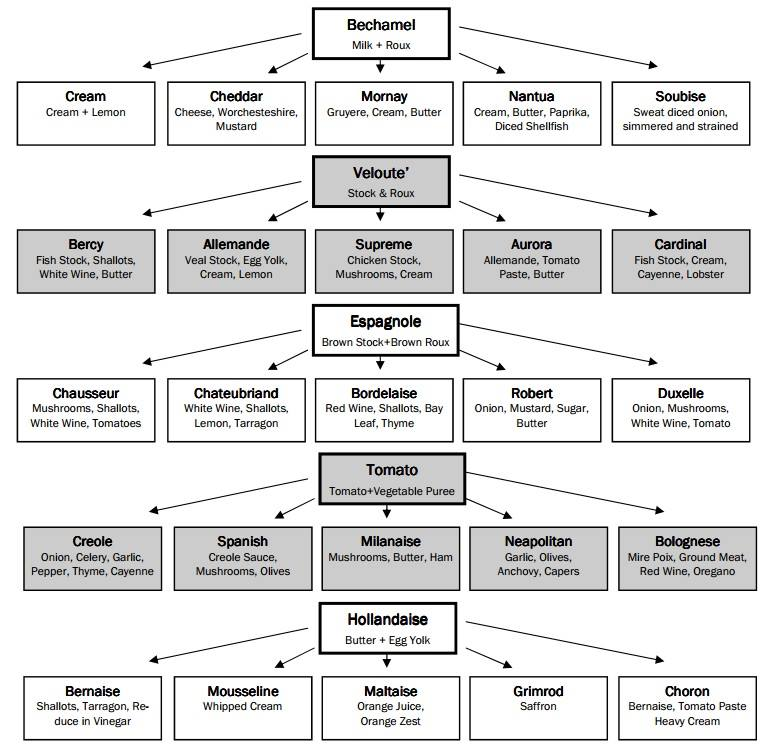
\includegraphics{rmds/images/saucer.jpg}

}

\caption{sovsene}

\end{figure}

Den skal laves til noget egen grafik.

\hypertarget{buxe6rnuxe6se}{%
\section{bærnæse}\label{buxe6rnuxe6se}}

50 - 100 gram smør pr person. 1-2 æggeblommer pr 100 gram smør (to hvis
små æg, en hvis store) Essens Hakket estragon salt hvid peber

Smelt smørret. Adskil fedt fra valle og gem vallen. Hav det lune klarede
smør stående i sovsekande. Smid æggeblommerne i saucieren. Tilsæt en
spiseskefuld vand pr blomme. Pisk til det skummer let. Tænd varmen,
middel til høj, og pisk konstant. Efter lidt tid ser du at æggene
emulgerer og vosker til dobbelt størrelse. Når du begynder at kunne se
bunden af saucieren når du pisker, tager du den af varmen og pisker et
par sekunder mere. Blommerne er nu emulgerede, og kan tage mod ret store
mængder smør uden at skille. Tilsæt smørret under piskning.

Smag til med saltm, peber, friskhakket estragon og essensen. Der skal en
til to spsk essens pr 100 gram smør. Sådan ca. det afhænger også af
essensen.

Kom først essensen i til sidst. Det gør det lettere at smage til. Og den
alve ph værdi i essensen kan gøre blommerne stive. Tilsæt lidt af vallen
hvis saucen er bleveet for tyk.

\hypertarget{choronsovs}{%
\section{Choronsovs}\label{choronsovs}}

Skal der laves mad til 14 personer i et lille køkken, alene, er der
grænser for hvor avancerede hovedretter man kan give sig i kast med. Når
der så samtidig stilles (selvpålagte) krav om at foretage sig noget i
køkkenet der kan levere en salve i den fortsatte kulinariske kamp med
lillebror, er sovsene et oplagt sted at indlede et felttog. Nogle simple
kartofler, en simpel grøntsag og en ko der er marineret. Og så en sovs
der hedder noget avanceret, og kan tage kegler.~

Så hermed et nyt våben i arsenalet, choronsovs. Eller Sauce Choron. Helt
simpelt, når først bearnaiserutinen er på plads.

En portion bearnaisesovs -- hjemmelavet fra bunden naturligvis --
tilsættes en spiseskefuld tomatpure. Hep! Enklere kan det vist ikke
gøres.~

En portion bearnaise her i huset er lavet på fire æggeblommer og en
pakke smør. Skaler selv op efter behov.

\hypertarget{de-andre-sovse}{%
\section{De andre sovse}\label{de-andre-sovse}}

\hypertarget{steaksovs}{%
\subsection{steaksovs:}\label{steaksovs}}

\begin{itemize}
\tightlist
\item
  1/4 cup sennepspulver, Colmans - det er så også den eneste jeg normal
  kan finde
\item
  2 spsk varmt vand
\item
  2 spsk risvins eddike - vi prøver nok også med hvidvinseddike
\item
  1/4 cup soyasovs
\end{itemize}

Bland sennepspulver med vandet, og lad det sætte sig et par minutter.

Tilsæt eddike og soyasovs, bland, og passer gennem finmasket si.

Bum. Den skulle blive bedre hvis den får lov at stå på køl mindst en
time.

Går også godt med andet - eg fisk.

\hypertarget{cherry-tomat-sovs}{%
\subsection{Cherry tomat sovs}\label{cherry-tomat-sovs}}

Fra Noma. Hvor de kalder den for ``Faster than you can boil pasta cherry
tomato sauce''

\begin{itemize}
\tightlist
\item
  30 ml oliven olie
\item
  2 fed hvidløg
\item
  200 gram søde cherry tomater
\item
  1½ spsk ``wild rose vinegar''.
\end{itemize}

Skær hvidløgene tyndt, tilføj dem til kold pande, med olivenolien.
Medium varme til de begynder at karamelisere. Tilsæt de hele tomater,
med et generøst drys salt. Låg på.

5-6 minutter senere er tomaterne sprængt og meget bløde. Stavblend til
du kan lide konsistensen. Tilføj eddike (mon ikke vi skal prøve med
balsamico), og smag til med mere eddike, salt og peber.

Foldes ind i kogt pasta, og serveres med et drys parmasan ost, et par
dråber olie og evt et frisk basilikumblad.

Serveres med 200-300 gram pasta (altså før det koges)

\hypertarget{pebersovs}{%
\subsection{Pebersovs}\label{pebersovs}}

Der skal udvikles yderligere. Den foreskrev oprindeligt 50 gram
peberkorn. Og det var for meget.

\begin{itemize}
\tightlist
\item
  2 små skaloteløg
\item
  olivenolie
\item
  25 gram syltede grønne peberkorn
\item
  2 teskeer sennep
\item
  7 dl okseboullion
\item
  1 sjat whiskey (prøv evt cognac i tstedet)
\item
  1 dl fløde
\item
  100 gram smør
\end{itemize}

skalotteløg hakkes og klares i olie. Peberkorn (knus ca 1/4 af dem med
en ske) skylles og tilsættes sammen med boullion og sennep. Koges ind
til ca. det halve.

tilsæt whiskey og fløde - kog et minuts tid ekstra.

Monter med smør, smag til med salt, sukker og peber.

Med 50 gram peberkorn, hvor intet blev mast, skulle der 2 dl fløde til,
og den var stadig ret heftig.

\hypertarget{ruxf8get-svampesauce}{%
\subsection{Røget svampesauce}\label{ruxf8get-svampesauce}}

\begin{itemize}
\tightlist
\item
  400 g blandede svampe - skåret i relativt tykke skiver (ca 5 mm)
\item
  olie
\item
  2 smadrede fed hvidløg
\item
  30 g smør
\item
  45 gram røget svampe garum
\item
  200 gram fløde
\item
  5 gram fint hakkede purløg
\item
  5 gram hakket persille
\item
  salt, peber og citronsaft
\end{itemize}

brun svampene i olien i sauterpande ved middel varme.

tilsæt smør til panden. tilføj hvidløg. rør godt rundt til smørret er
smeltet og alt er godt blandet. ca. 2 minutter.

Steg svampene et par minutter til. Hæld garum i, og steg lidt videre,
til væsken er optaget af svampene. ca. 3 minutter. tilsæt fløde og lad
simre til fløden er reduceret til halvdelen og blevet tykkere. Tilsæt
krydderuerter og smag til med salt, peber og citron.

Også brugbar som pastasovs.

\hypertarget{bistro-sovs}{%
\section{Bistro sovs}\label{bistro-sovs}}

Her er vi i de ægte sovse. En opskrift fra Brødrene

\begin{itemize}
\tightlist
\item
  1 1/4 dl hvidvin
\item
  4 æggeblommer
\item
  1 pakke smør
\item
  1 lille skalotteløg - hakket
\item
  1 bundt purløg - klippet
\item
  1 øko citron
\item
  1 tsk Sennep
\item
  1-2 spsk vineddike. Gerne sherry
\end{itemize}

Eddike, hvidvin og løg koges ind til stort set intet. Æggeblommer og
sennep piskes sammen med essensen. Så piskes det klarede, lune, smør i
ganske som en bærnæse. Smag til med citron, salt og peber. Principielt
bør det nok være hvid peber\ldots{} Men det er vi for dovne til. Evt
også lidt mere eddike. Rør purløg i, og server.

\hypertarget{portvinssauce}{%
\section{Portvinssauce}\label{portvinssauce}}

\begin{itemize}
\tightlist
\item
  1 gulerod
\item
  1 løg
\item
  1 fed hvidløg
\item
  frisk timian
\item
  1 spsk olie
\item
  2 dl portvin
\item
  2 dl rødvin
\item
  4 dl oksefond
\item
  ½ dl stegesky eller hvad du nu har fra resten af madfremstillingen
\item
  salt, pber, citronsaft og gastrik
\item
  20 gram koldt smør i tern
\end{itemize}

rengør og hak grøntsagerne. Sauter dem i olien. Tilsæt portvin, rødvin
og hakket frisk timian. Kog ind til det halve. Hæld oksefonden ved, og
kog igen ind til det halve. Tilsæt stegeskyen. Smag til med salt, peber,
citronsaft og gastrik. Tag sovsen af varmen, sigt den og pisk smørtern i
(et ad gangen). Server.

\hypertarget{balsamico-sovs}{%
\subsection{Balsamico sovs}\label{balsamico-sovs}}

\begin{itemize}
\tightlist
\item
  2 spsk rørsukker
\item
  2 spsk balsamico eddike
\item
  1½ dl kalve eller kyllingefond
\item
  2½ dl piskefløde
\item
  Salt, peber, lidt maizenajævner
\end{itemize}

Smelt sukkeret, rør eddiken i. Rør fonden i til sukkeret er opløst. Rør
piskefløden i, kog igennem. Juster tykkelsen med lidt maizena, og smag
til med salt og peber.

\hypertarget{ostedip}{%
\subsection{Ostedip}\label{ostedip}}

Ikke rigtig en sovs. Men her er den.

\begin{itemize}
\tightlist
\item
  25 g smør
\item
  2 spsk mel
\item
  2 dl mælk
\item
  200 g revet cheddar
\item
  1 fed hvidløg - kvast
\item
  ½ chili eller tørrede chiliflager. Eller bare stødt chili.
\item
  1 tsk NaCl
\item
  1 tsk paprika
\end{itemize}

Smelt smørret med krydderier, salt og hvidløg

Bag op med mel og mælk.

Tilsæt osten og varm op til den er helt smeltet.

Smag til, og nej, der skal nok ikke mere salt i!

Juster tykkelsen med mælk, og server så snart den er færdig. Ellers
serverer du ikke en dip, men en klods.

\hypertarget{andesovs.-a-lorange}{%
\section{Andesovs. A l'orange}\label{andesovs.-a-lorange}}

Hvis det ikke skal være en helt traditionel, fed, brun andesovs.

\begin{itemize}
\tightlist
\item
  Saft af tre appelsiner
\item
  Skal af en appelsin (så den skal ikke være overfladebehandlet\ldots)
\item
  Saft og skal af 1 lille citron (ej heller overfladebehandlet)
\item
  6 dl andefond
\item
  3 spsk cognac
\item
  2 spsk sukker
\item
  2 spsk æbleeddike
\item
  Salt
\end{itemize}

Skallen af citrusfrugterne (skræl, ikke riv. Og lad være med at få for
meget af det hvide med) skæres i tynde strimler.

Bring vand og en lille smule salt i kog, og blancher skallerne i 3
minutter. Genta processen med frisk vand, så de bliver blancheret to
gange. Lad dem dryppe af.

Pres saften af citrusfrugterne, og hæld dem i en gryde med fond og
cognac. Du kan også bruge calvados. Men vent med varmen.

Hæld sukker i en separat kaserolle, og smelt til en gylden karamel. Ej
mørk! Tilsæt eddike og lad det boble sammen.

Hæld gastrikken, for det er sådan en du har lavet, ned i gryden med fond
og citrussaft, og lad nu blandingen koge ind til ca. det halve. Smag til
med salt, cognac og evt lidt mere appelsinsaft.

Smid halvdelen af de blancherede citrusskaller i sovsen. Den anden
halvdel kan bruges som pynt på anden.

\hypertarget{suxf8ren-villemoes-tomatsovs}{%
\section{Søren villemoes tomatsovs}\label{suxf8ren-villemoes-tomatsovs}}

Brug flåede tomater fra Mutti. Eller bedre. Koncentreret tomatpasta på
tube fra samme mærke.

Varm olivenolie op i sauterpande eller kasserolle med 2-3 fed pressede
hvidløg og lidt chilipulver. Mængden af sidstnævnte afhænger af styrken.
Den skal ikke brænde igennem, men blot give et lille pift og være
smagsforstærkende. Når det har stegt lidt uden at branke, og mistet den
ferske duft, tilføjes 1-2 spsk tomatpasta. Steg det med et minuts tid
til en anelse karamelliseret. Tilføj de flåede tomater. Lidt vand i
dåsen for at åf det sidste med ud. Sænk varmen til lav, låg på. Lad
simre i en times tid - tilføj evt lidt vand hvis det bliver for tørt.
Efter en times moses tomaterne med en ske. Og der smages til med
gavmilde mængder salt.

\hypertarget{kold-falsk-bearnaisesovs}{%
\section{Kold (falsk) bearnaisesovs}\label{kold-falsk-bearnaisesovs}}

Det har intet med bearnaisesovs at gøre. Men det er ret godt, smager
derhenad, og går fremragende til et godt stykke kød.~

\begin{itemize}
\tightlist
\item
  2 dl creme fraiche 18\%
\item
  2 spsk estragoneddike
\item
  3 spsk sød sennep
\item
  1 bundt hakket estragon
\item
  Salt, peber og evt. lidt citronsaft
\end{itemize}

Rør creme fraiche, eddike og sennep sammen. Det kan gøres i god tid
inden servering. Smag til med salt, (hvid) peber og lidt citronsaft
(hvis du har. Det går fint uden). Rør den hakkede estragon i lige inden
servering.

\hypertarget{gorgonzola-sovs}{%
\section{Gorgonzola sovs}\label{gorgonzola-sovs}}

Det er ikke min opskrift. Den ære tilfalder Niels Ipsen, der delte den
på verdens bedste facebookgruppe, Gudemad.~ Jeg har så heller ikke
prøvet den endnu, men det skal ske snart!

Varm en centimeter olivenolie op i en gryde (jeg vil nok bruge en
kasserolle, ellers er det ret meget sovs). Smid en stor klods gorgonzola
i olien, og lad den smelte. Saml sovsen med en stor klat creme fraiche
38\%.

Det forlyder at den er god til pasta. Og det skal klart prøves!

\hypertarget{bearnaise-sifon}{%
\section{Bearnaise sifon}\label{bearnaise-sifon}}

Gårsdagens restemad fik lige et molekylær gastronomisk pift -- bearnaise
sifon.~

Der er researchet på adskellige sites, Google Translate har oversat fra
både fransk og tysk. Så inspirationen kom mange steder fra. Ingen linket
til, ingen glemt.

Opskriften der blev fulgt er som følger:

250 g klaret smør (250 g smør blev klaret. Vi gider ikke veje smørret
når det først er klaret) 4 æggeblommer (2 bægre pasteuriserede blommer)
2 spsk bearnaise essens (ja, jeg var doven og gad ikke lave den selv)

De tre ingredienser blev hældt på sifonen. Der blev rystet grundigt og
tilsat to skud lattergas. Og så stod sifonen og hyggede sig i 60 grader
varmt vand en time.

Der var lige lovligt meget tryk på sifonen. Så næste gang prøver jeg med
et enkelt skud. Og så skilte skummen også ret hurtigt. Den får nok en
knivspids agar agar næste gang. Men det var et fint gult skum, der
smagte som forventet. At vi så havde bearnaiseskum ud over det hele er
en anden sag.

\hypertarget{whisky-beurre-blanc}{%
\section{Whisky Beurre Blanc}\label{whisky-beurre-blanc}}

50 ml whiskey eddiek 100 ml hvidvin 200 gram smør 4 peberkorn 1
laurbærblad 1 skalotteløg salt

Bring hvidvin, eddike, peberkorn, laurbær og finthakket løg i kog.
Reducer til halvdelen. Sigt. Bring reduktionen til simren. Pisk 200 gram
kold smør, i terninger, i. tag gryden af når du pisker smørret i. Pas på
varmen, det skiller relativt let. Smag til med salt, peber og whiskey.
Og hold varm. Egner sig ikke til genopvarmning, og serveres kort efter
produktion.

\bookmarksetup{startatroot}

\hypertarget{kondimenterne}{%
\chapter{kondimenterne}\label{kondimenterne}}

\hypertarget{syltede-ruxf8dbeder}{%
\section{Syltede rødbeder}\label{syltede-ruxf8dbeder}}

\hypertarget{syltede-champignon}{%
\section{Syltede champignon}\label{syltede-champignon}}

\begin{itemize}
\tightlist
\item
  500 gram hvide champignons, rensede og rodskårne
\item
  2 dl mørk balsamico
\item
  2 dl olivenolie
\item
  1 spsk salt
\item
  20 sorte peberkorn
\item
  5-8 laurbærblade
\end{itemize}

Rør alt andet end svampene sammen - grundigt Læg svampe i sterilt glas,
hæld lage over, og lad trække i to døgn. Spises som tilbehør til grillet
kød, som tapas elleer i salater

\hypertarget{trykkogerketchup}{%
\section{Trykkogerketchup}\label{trykkogerketchup}}

efter www.hippressurecooking.com/pressure-cooker-ketchup-recipe og Dansk
Kemi 2020 (6) p.~38 - 39, ved Jens Folke

\begin{itemize}
\tightlist
\item
  1 kg blommetomater skåret i kvarte
\item
  15 g paprika
\item
  5 g salt
\item
  1 g stødt kanel
\item
  1 g nelliker stødt
\item
  2 g hvidløgspulver
\item
  2 g sellerifrø
\item
  10 g dijonsennep
\item
  15 g honning
\item
  80 g rosiner
\item
  1/4 zittauerløg
\item
  85 ml æbleeddikke
\item
  15 g majsstivelse rørt ud i 15 ml vand
\end{itemize}

Kan yderligere krydres med chili, røget paprika, æble, korianderfrø
m.m.m

Smid alt undtagen majsstivelse og vand i trykkogeren.

Mos tomaterne nok til at væsken når op på trykkogerens minimumsbehov
bring trykkogeren under tryk, når den når 2 atmosfærer, lad koge i 5
minutter Tag trykket af, og lad det koge ind i 10 minutter - reduceres
til knap halvdelen.

Bland majsstivelse i vand, og hæld det i - lad det koge med.

Smadr blandingen med stavblender - passer gennem sigte.

\hypertarget{skalottemarmelade}{%
\section{Skalottemarmelade}\label{skalottemarmelade}}

giver 1½ kop

\begin{itemize}
\tightlist
\item
  Neutral olie
\item
  1 kg skalotter - pillet og hakket
\item
  3/4 teske salt
\item
  ½ kop sukker
\item
  6 spiseskeer malteddike - eller anden eddike.
\end{itemize}

Olie i sauterpande. Løg og salt i pande. ``kog'' under låg i ca. ti
minutter. Rør undervejs, til løgene er klare skru ned for varmen og tag
låget af. tilsæt sukker og 1 spsk vand. simrer i 30 minutter. deglacer
med 1 spsk vand efter behov. rør derefter fire spsk eddike i. simrer
videre i 10-15 minutter, til konsistensen er jammy. rør den resterende
eddike ind, og sluk for varmen. Smag til. Hæld på glas (skoldet etc)

\hypertarget{fars-nylon}{%
\section{Fars nylon}\label{fars-nylon}}

Aka 1000 øers dressing

\begin{itemize}
\tightlist
\item
  Mayo - svarende til af en æggeblomme og 3 dl olie
\item
  1 spsk creme fraiche
\item
  1 spsk tomatpure
\item
  1 tsk engelsk sovs
\item
  1 knivsspids paprika
\item
  1 smule tabasco
\item
  1 smule cognac
\item
  1 smule sukker
\end{itemize}

Det hele blandes sammen.

\hypertarget{worcestershire-sauce---engelsk-sovs}{%
\section{Worcestershire Sauce - Engelsk
sovs}\label{worcestershire-sauce---engelsk-sovs}}

Eller hvad pokker det nu hedder\ldots{}

500 ml Æble eddike 4 fed hvidløg 120 g skalotteløg 30 g ansjosfilleter
60 g honning 60 g rørsukker eller melasse 60 g tamarind paste 2 tsk
chilipulver 1 tsk stødte nelliker

Alt smides i en gryde, og der stavblendes til det er så smooth som
muligt.

varm op ved medium varme til den koger. Skrug ned til lav varme og lad
simre i 15 minutter under omrøring.

Herfra er der to metoder:

\begin{enumerate}
\def\labelenumi{\arabic{enumi}.}
\tightlist
\item
  Filtrer gennem kaffefilter. Lad det dræne en times tid. Rør let i
  pastaen så det meste kommer igennem. (brug evt først det fine
  nylonfilter).
\end{enumerate}

Tilsæt tre tsk af filterkagen til filtratet, ryst grundigt og hæld
straks på rengjorte skoldede (evt atamonskyllede) flasker. Opbevar mørkt
og køligt (men ikke i køleskabet). Lad den lagre mindst 2 måneder, helst
18 måneder.

Filterkagen kan med fordel gemmes og tilsættes supper, gryderetter eller
andet godt.

\begin{enumerate}
\def\labelenumi{\arabic{enumi}.}
\setcounter{enumi}{1}
\tightlist
\item
  Hæld sovsen direkte på rengjorte, skoldede, evt. atamonskyllede
  flasker. Den lagres ligeså længe. Der er frit valg ang. filtrering
  efter den har lagret.
\end{enumerate}

\hypertarget{whiskey-bacon-jam}{%
\section{WHISKEY BACON JAM}\label{whiskey-bacon-jam}}

\begin{itemize}
\tightlist
\item
  ½ kg bacon - i tern
\item
  2 store løg, tyndt skåret
\end{itemize}

• 3 cloves garlic, minced • ¼ cup brown sugar • 3 tbsp whiskey or
bourbon • 2 tbsp maple syrup • 2 tbsp balsamic vinegar • 1 tsp black
pepper • ¼ tsp cayenne pepper • ¼ cup water Instructions: 1. In a large
skillet, cook bacon over medium heat until crispy. 2. Remove bacon with
slotted spoon, reserving 2 tablespoons of bacon fat in pan. 3. Add
onions to the pan and cook over medium-low heat until caramelized, about
20-25 minutes. 4. Add garlic and cook for 1 minute until fragrant. 5.
Return bacon to pan and add brown sugar, whiskey, maple syrup, balsamic
vinegar, and seasonings. 6. Add water and simmer until mixture thickens,
about 10-15 minutes. 7. Let cool slightly, then pulse in food processor
to desired consistency. 8. Allow to cool completely before transferring
to jars. 9. Perfect for burgers, grilled cheese sandwiches, crackers
with cheese, or roasted meats. 10. Store in refrigerator for up to 2
weeks.

\hypertarget{ketchup}{%
\section{Ketchup}\label{ketchup}}

En af basisfødevarerne. Beauvais smager af tysk rasteplads. Heinz er
bedst. Men er et amerikansk mærke, og vi er ikke fans af lande der
styres af psykotiske bavianer med et ketaminmisbrug.

Så hvorfor ikke lave det selv?

\begin{itemize}
\tightlist
\item
  1 løg
\item
  3 fed hvidløg
\item
  1 (mad)æble
\item
  1 kg tomater
\item
  ½ frisk, rød, mild chili
\item
  Olivenolie
\item
  2 spsk tomatpure
\item
  2 dl vand
\item
  2 spsk sukker
\item
  3 spsk eddike
\item
  Salt og peber
\end{itemize}

Pil løg og hvidløg, skyl og skræl æblerne, skyl tomaterne.

Rens chilien, fjern især frøene!

Skær alt i grove tern. Det skal blendes, så det er ok at være doven.
Steg (hvid)løg i en gyde i 3-4 minutter i en sjat olie

Tilsæt æbler, tomater, tomatpure og vand, og lad det hele simre i 10-15
minutter under låg. Blend det godt igennem, og smag til med sukker,
eddike, salt, peber og evt cayennepeber.

\hypertarget{havtorn-sirup}{%
\section{Havtorn sirup}\label{havtorn-sirup}}

4 dl havtorn. 4 dl sukker 3 dl vand. En stjerneanis Det hele samles i en
gryde, bring i kog og opløs sukkeret. Kog dernæst i 5 minutter.~ Tag
gryden af varmen og lad det trække i en times tid inden det filtreres -
gerne gennem noget klæde.~ Kog yderligere ind til det har den ønskede
konsistens Hæld på atamon-skyllet flaske.

\hypertarget{suxe5-er-det-syltetid-abrikoser-og-mandler}{%
\section{Så er det syltetid -- abrikoser og
mandler}\label{suxe5-er-det-syltetid-abrikoser-og-mandler}}

Hvordan resultatet bliver aner jeg ikke. For gryden er stadig på
blusset.

94 g smuttede hele mandler 218 g halverede soltørrede abrikoser Korn af
1 vanillestang. De to halvdele kommer med i sylteglasset 15 ml amaretto
2,5 dl rørsukker 2,5 dl vand Et lille nip chilipulver

Det hele smides i en kasserolle, og koger op. Når det er oppe at koge,
lader jeg det koge videre til temperaturen når 107 grader. Det skulle
give en relativt tyk sirup. Når jeg har postet dette, skolder jeg et ½
liters sylteglas, og skyller det i en hættefuld atamon. Atamonen ryger i
vasken bagefter, men glasset bliver ikke rystet for voldsomt, der må
godt være et par dråber tilbage i glasset, af hensyn til holdbarheden.

\hypertarget{syltetid-iii-hasselnuxf8dder-i-lidt-lakrids}{%
\section{Syltetid III -- Hasselnødder i lidt
lakrids}\label{syltetid-iii-hasselnuxf8dder-i-lidt-lakrids}}

Vi fortsætter -- kæresten er nemlig til kor, så der er ikke så meget
andet at tage sig til

Det var en stor pose hasselnødder, og de endte ikke alle blandt fignerne
i går. Så derfor:

Hasselnødder nok til at fylde (næste) et ½ liters sylteglas 2½ dl
rørsukker 2½ dl vand 1 tsk lakridspulver

Koges op, og ind, til temperaturen er 107 grader. Hældes på skoldet og
atamon-skyllet glas. HSKDV. Og at dømme efter første smagsprøve, er
lakridsen perfekt doseret.

\hypertarget{syltetid-iv-figner-og-ruxf8dvin}{%
\section{Syltetid IV -- Figner og
rødvin}\label{syltetid-iv-figner-og-ruxf8dvin}}

Og søreme om ikke vi fortsatte -- det er utroligt hvad man kan klare
mens man taler i telefon med sin mor, bare man har et headset.

305 g tørrede figner 2½ dl rørsukker 1 dl rødvin (en barbaresco i dette
tilfælde -- det hvad hvad jeg alligevel havde trukket op) 1½ dl vand

Og nu skulle rutinen være på plads. Koge op -- relativt roligt -- til
107 grader, på skoldede og atamonskyllede glas. En hurtig prøvesmagning
gjorde at den fik et lille skvæt ekstra rødvin fra glasset, så måske er
det 1,25 dl rødvin den skal have i stedet. Og tag det nu roligt hvis det
ikke er præcist 305 gram figner. 300 gram er sikkert ok, det var bare
hvad der passede i mit ½ liters sylteglas.

\hypertarget{syltetid-figner-og-hasselnuxf8dder}{%
\section{Syltetid -- figner og
hasselnødder}\label{syltetid-figner-og-hasselnuxf8dder}}

To portioner på en dag -- men så har vi heller ikke flere sylteglas, så
nu stopper det.

Det krævede en længere debat med kæresten, under brug af boolske
operatorer og whiteboardtavle. Men til sidst endte det med figner og
hasselnødder.

216 g tørrede figner 77 g hasselnødder 2 kanelstænger 2½ dl rørsukker 2½
dl vand 20 ml Morgan rom

Igen, hele svineriet i kasserollen, op med varmen (i moderat tempo,
kanelstængerne skal have lidt tid til at trække), og koge ind til
temperaturen når 107 grader. Skoldet glas skyllet i atamon. Så ser vi om
det også passer med ½ liter denne gang.

\bookmarksetup{startatroot}

\hypertarget{specialiteterne}{%
\chapter{Specialiteterne}\label{specialiteterne}}

\hypertarget{konfiterede-hvidluxf8g}{%
\section{Konfiterede hvidløg}\label{konfiterede-hvidluxf8g}}

Et lille sylteglas fyldes med pillede hvidløg

Salt kommes i (hvor meget?) sammen med krydderier.

rosmarin og rosenpeber skulle være godt.

Så fyldes glasset med en god olie og låget lukkes til.

Sous vides det i 3-4 timer på 87 grader

\hypertarget{saltede-uxe6ggeblommer}{%
\section{Saltede æggeblommer}\label{saltede-uxe6ggeblommer}}

Fyld et par centimeter fint (IKKE groft) salt i en bøtte. Skil blommer
fra æg, og placer dem på saltet. Dæk fuldsændigt med salt Lad stå i
køleskabet 8 timer. Pil æggeblommerne op af saltet, skyl dem i koldt
vand, tør dem. Og tør dem i ovnen vad 60 grader - 2 timer er for lidt,
opskriften sagde også 3. De er for gummiagtige, så de skal have længere
end det.

Målet er at de skal kunne rives. Så de skal være ret hårde og tørre.

\hypertarget{sous-vide-kold-kaffe}{%
\section{sous vide kold kaffe}\label{sous-vide-kold-kaffe}}

\begin{itemize}
\tightlist
\item
  ½ cup (så volumen mål) groft kværnet kaffe
\item
  4 cup vand
\end{itemize}

kaffe og vand i vandtæt syltetøjsglas. Sousvides i 2-4 timer ved 150
grader F.

Filtrer, og server hældt over is, eller opbevar på køl i en uges tid.
Overvej om den skal fortyndes.

\hypertarget{kaffesmuxf8r}{%
\section{Kaffesmør}\label{kaffesmuxf8r}}

Det her skal prøves!~

Oversættelsen må være ``kaffesmør'', men originalen kalder det for~Uber
fantastic Coffee
Butter:~http://www.instructables.com/id/Uber-fantastic-Coffee-Butter/.

\begin{itemize}
\tightlist
\item
  En spsk fintmalet kaffe
\item
  En spsk jordnøddesmør
\item
  En tsk honning eller sukker.
\end{itemize}

De skriver ikke noget om hvilken slags jordnøddesmør der skal til. Men
jeg vil gætte på at det ikke skal være crunchy.

\hypertarget{uxe6rtepesto}{%
\section{Ærtepesto}\label{uxe6rtepesto}}

\begin{itemize}
\tightlist
\item
  2 dl ærter - friske er selvfølgelig pr definition bedst. Men så skal
  de blancheres først.
\item
  1 fed hvidløg
\item
  1 dl mandler (smuttede)
\item
  ½ dl olivenolie
\item
  2 spsk citronsaft
\item
  salt og peber
\end{itemize}

Rist mandlerne på panden til de er gyldne og sprøde. Gerne med lidt
salt.

Alle øvrige ingredienser stavblendes, og der smages til med salt, peber
og citronsaft. Hak mandlerne og rør dem i ærtepestoen.

\hypertarget{huxe5ndsprit}{%
\section{Håndsprit}\label{huxe5ndsprit}}

Ja, det er faktisk alvorligt. Måske ikke for dig. Men hvis fem procent
af de der bliver smittede med Corona-virusen skal indlægges, og
halvdelen af landets befolkning på 5,8 millioner bliver smittet - så er
det 145.000 mennesker der skal indlægges. Hvordan tror du selv at det
danske sundhedsvæsen vil håndtere den opgave?

Anyway. Flydende håndsprit kan laves efter disse opskrifter. En af
dagene ser jeg om jeg kan få skruet en opskrift på en gel sammen.

Du skal bruge:

\begin{itemize}
\tightlist
\item
  99\% isopropylalkohol eller 93\% husholdningssprit.
\item
  Glycerin
\item
  Brintoverilte 3\%
\item
  Vand
\end{itemize}

Det hele kan findes hos en materialist. Hvis du kan finde sådan en.
Matas er jo en parfumeforretning nu.

40 ml brintoverilte blandes med 15 ml glycerin.

Hvis du bruger husholdningssprit fortyndes den blanding til 160 ml med
vand. Og fortynd den blanding til 1 liter med husholdningssprit.

Hvis du bruger isopropylalkohol, fortyndes blandingen til 240 ml med
vand. Og den blanding fortyndes så til 1 liter med isopropylalkohol.

\bookmarksetup{startatroot}

\hypertarget{rester}{%
\chapter{Rester}\label{rester}}

Vi skal af med resterne

\hypertarget{standardmuxe5der}{%
\section{Standardmåder}\label{standardmuxe5der}}

\begin{itemize}
\tightlist
\item
  Standard pastabix - Se under pastaretterne
\item
  Bixemad
\end{itemize}

\hypertarget{gratin}{%
\section{Gratin}\label{gratin}}

Dette er basisopskriften. Den skal bruges til at skaffe os af med
rester.

\begin{itemize}
\tightlist
\item
  100 g smør
\item
  150 g mel
\item
  3 dl grøntsagsbouillon
\item
  3 dl sødmælk
\item
  8 æg
\item
  salt, peber, rasp
\end{itemize}

mindst 50 gram rester, men den kan sagtens trække en del mere. Skær
resterne i mindre stykker

Smelt smør, rør sammen med mel. Lav grundlæggende en opbagt sovs med
væsken. Del æggene, tag gryden af varmen, og rør blommerne i,.

Pisk hviderne stive, vend halvdelen i gryden sammen med fyldet.

Vend resten af hviderne i. Smør et fad/skål og drys med rasp. drys rasp
over gratinen, bag nederst i ovnen ved 175 grader i ca. 1 time. Server
med smeltet smør.

\hypertarget{kartoffelmosfrikadeller}{%
\section{Kartoffelmosfrikadeller}\label{kartoffelmosfrikadeller}}

Eller - det har intet med frikadeller at gøre, frikadeller skal laves af
de dele af svinet der er så ringe, at vi ikke kan sælge det til
englænderne, ellers er det ikke frikadeller.

500 gram kartoffelmos

1 revet løg

1 æg

3-4 spsk mælk

2-3 spsk hvedemel

4-5 spsk rasp

salt og peber

Alt røres sammen, massen formes til frikadelle-formatet, og steges 2-3
minutter på hver side i rigeligt smør, til de er gyldne. Læg dem
tilafdrypning på køkkenrulle. Server som tilbehør.

\bookmarksetup{startatroot}

\hypertarget{hapsere-tapas-med-videre.}{%
\chapter{Hapsere, tapas med videre.}\label{hapsere-tapas-med-videre.}}

\hypertarget{ruxf8dbedesyltede-uxe6g}{%
\section{Rødbedesyltede æg}\label{ruxf8dbedesyltede-uxe6g}}

\begin{itemize}
\tightlist
\item
  6 æg - skal du bruge 8, skal der formentlig skaleres op
\item
  1 rødbede
\item
  3½ dl æblecidereddike
\item
  2 dl ale
\item
  1 spsk hele sennepsfrø
\item
  4 laurbærblade
\item
  3 stk hel allehånde
\item
  10 peberkorn
\item
  1 tsk tørret chili
\item
  2 spsk sukker
\end{itemize}

Kog æggene 7-8 minutter, isvand, pil. Skræl rødbeden og skær den i tern.
Husk gummihandsker! Kog rødbeden med alle øvrige ingredienser i 7-10
minutter. Skold et sylteglas, læg de kolde (!) æg i. Hæld den (HELT)
afkølede lage over, og ryst let så æggene er dækket på alle sider. Sæt
på køl og i 4 døgn.

\hypertarget{toskanske-buxf8nner}{%
\section{Toskanske bønner}\label{toskanske-buxf8nner}}

Jeg har aldrig forstået hvorfor de der hvide bønner skulle kunne bruges
til andet end at kaste efter folk.

Indtil vi fik en anretning på en restaurant i Firenze vi havde fundet i
en reklametryksag fra et dækfirma.

Fagioli all'uccelletto

\begin{itemize}
\tightlist
\item
  600 gram hvide bønner (helt oprindeligt - cannellini)
\item
  olivenolie
\item
  lidt salvie blade
\item
  to fed hvidløg
\item
  2 spsk tomat pure
\item
  4 ferske svinepølser (og her dur det altså ikke med grillpølser\ldots)
\item
  salt og peber
\end{itemize}

Bønnerne skal ligge i blød. Og så skal de koges. Gerne i noget bouillon.

Så varmer vi et par spiseskeer olie op på en pande med hvidløget - bare
lad skindet være på dem, og knus dem med hånden - og salvien

Når olien har taget smag af hvidløget, og salvien er blevet sprød,
hælder vi bønnerne op i panden, sammen med en god sjat af deres
kogevand. Tilføjer tomatpastaen, rører rundt og koger ved lav
temperatur. Lad dem simre i 20 minutter, pil pølserne ud af deres skind,
og smid dem i. Lad det yderligere simre til pølserne er færdige. Server
med brød.
https://www.visittuscany.com/en/recipes/fagioli-alluccelletto-tuscan-style-beans-recipe/1111

\hypertarget{gougeres}{%
\section{Gougeres}\label{gougeres}}

Giver to fulde bageplader!

\begin{itemize}
\tightlist
\item
  100 g hvedemel
\item
  90 g smør
\item
  1 dl vand
\item
  1 dl sødmælk
\item
  1⁄2 tsk. groft salt
\item
  1⁄2 tsk. sukker
\item
  3 store æg L/XL, sammenpiskede (ca. 180 g)
\item
  100 g revet gruyère ELLER 150 g frisk gedeost samt kværnet sort peber
\end{itemize}

\begin{enumerate}
\def\labelenumi{\arabic{enumi}.}
\item
  Forvarm ovnen til 200° uden varmluft. Beklæd to bageplader med
  bagepapir.
\item
  Sigt melet -- gerne ned på et stykke bagepapir, da det så kan hældes
  hurtigt i gryden.
\item
  Smelt smørret sammen med vand, mælk, salt og sukker i en gryde ved
  moderat varme. Når smørret er smeltet, bringes det hele i kog ved høj
  varme og tages straks af varmen. Hæld det sigtede mel i gryden, og rør
  med en træske, indtil det bliver til en fast, blød dej uden klumper,
  der slipper gryden.
\item
  Sæt gryden tilbage på kogepladen på svag varme for at 'riste' dejen i
  et par minutter. Rør forsigtigt i dejen mens den ristes, og undlad at
  skrabe i bunden af gryden. Der vil sætte sig et meget tyndt lag dej,
  som ikke skal blandes sammen med resten af dejen igen.
\item
  Hæld dejen i en skål, og lad den køle lidt af (i ca. 5 minutter). Hvis
  du bruger røremaskine, kan du med fordel hælde dejen i røreskålen og
  lade den køre rundt med 'det flade piskeris' på lav til
  mellemhastighed. På den måde køles dejen hurtigt.
\item
  Tilsæt de sammenpiskede æg ad tre omgange, og rør energisk efter gang
  for at få massen homogen. På røremaskine røres fortsat med lav til
  mellemhastighed med det flade piskeris. Når æggene tilsættes, vil
  dejen først se ud som om den skiller, men vil samle sig igen efter
  omrøring.
\item
  Fortsæt med at røre i dejen i nogle minutter, så den bliver godt
  elastisk. Dejen er klar når den er glat og skinnende.
\item
  Tilsæt revet gruyère eller snuldret gedeost (samt evt. peber eller
  krydderurter).
\item
  Overfør dejen til bagepladen med sprøjtepose, skeer eller en isske.
  Sæt små klatter på størrelse med en femmer til hors d'oeuvre eller
  store, hvis de skal spises som mellemmåltid.
\item
  Lav et kryds (gittermønster) på toppen af hver gougère med en gaffel
  dyppet i vand, så hæver de flottere i ovnen.
\item
  Sæt bagepladen i den varme ovn, og skru så ned til 170°. Lad dem bage
  i mindst 20 minutter uden at åbne ovndøren. Bagetiden afhænger af
  størrelsen. De er færdige, når de er jævnt lysebrune. De må gerne
  bages lidt mindre end vandbakkelser, som skal fyldes med creme. De er
  nemlig lækrest, hvis de er svampede indeni. TIP: Sæt gerne en ekstra
  bageplade i ovnen under pladen med vandbakkelser, så de ikke bliver
  brændte i bunden.
\end{enumerate}

\hypertarget{hummus}{%
\section{Hummus}\label{hummus}}

En dåse kikærter (vægt drænet?) En toppet spiseskefuld tahin Citronsaft
1 tsk spidskommen ½ dl koldt vand en isterning 3 spsk olie salt og peber

\hypertarget{bagt-camenbert}{%
\section{Bagt camenbert}\label{bagt-camenbert}}

I airfryer. Et stk camembert. Ikke en af de helt store - ikke en af de
helt små.

Skær tern i overfladen af osten, en centimeters penge på hver led. Pensl
med trøffelolie, hakket frisk timian, honning og chili. Noget mere end
man lige tror.

Bag i airfryeren ved 160 grader i 12 minutter. Lækkert.

\hypertarget{cheeseburger-buket}{%
\section{Cheeseburger buket}\label{cheeseburger-buket}}

tortillas smøres med hakket kød, og skæres i halve. En trekant
cheddarskive lægges på (bred side mod rundingen i tortillaen. Tortillaen
rulles til et kræmmerhus, og placeres i en rundform. 12 stykker eller
deromkring. i ovnen til kødet er tilberedt. Rdys med hakkede rødløg,
hakkede cornichoner og server med ostesovs.

Jeg er skeptisk overfor det med det rå kød. Så jeg steger det
først\ldots{}

\hypertarget{salte-mandler}{%
\section{SALTE MANDLER}\label{salte-mandler}}

250 gram mandler 250 ml vand 75 g salt

Kog vandet, tilsæt salt, og rør til det er opløst. Tag vandet af
blusset, og tilsæt mandlerne. Lad mandlerne trække i 20 minutter. Sigt
vandet fra, og tør mandlerne i ovnen ved 150 grader i 20 minutter. Lad
mandlerne køle af i ovnen.

\hypertarget{uxf8l-ost-dip}{%
\section{Øl-ost dip}\label{uxf8l-ost-dip}}

fra blizzard kogebogen

Cheddar-Beer Dip Bake time: 15 mins Makes: 1 batch Pairs well with:
Essential Brewfest Pretzels, and Spicy Vegetable Chips 2 tablespoons
salted butter 2 tablespoons flour 1 cup pale low-hop beer, such as a
pilsner ½ cup milk ½ teaspoon mustard ½ teaspoon garlic powder ½
teaspoon paprika Dash of Worcestershire sauce 3 cups sharp cheddar
cheese, shredded Salt and pepper to taste In a medium frying pan, melt
the butter over medium heat. Whisk in the flour and cook for a minute or
two, until the mixture has turned a nice golden color. While whisking,
gradually pour in the beer then the milk, both of which should thicken
as they heat. Remove from heat and stir in the spices, Worcestershire
sauce, and the cheese. Let the cheese melt; season to taste with salt
and pepper.

\bookmarksetup{startatroot}

\hypertarget{supperne}{%
\chapter{Supperne}\label{supperne}}

\hypertarget{luxf8gsuppe}{%
\section{Løgsuppe}\label{luxf8gsuppe}}

\begin{itemize}
\tightlist
\item
  1½ kg løg
\item
  3-400 g gruyere eller comtè ost
\item
  1-1½ l oksebouillon
\item
  1 glas hvidvin
\item
  1 lille glas cognac
\item
  2-3 stk. laurbær
\item
  1 kvist frisk timian
\item
  2-3 spsk. smør
\item
  8-10 stk. sorte peberkorn
\item
  2 spsk. hvedemel
\item
  1 flute
\end{itemize}

Pil og skær løgene tyndt. Svits dem langsomt i rigeligt smør og en sjat
olivenolie, til de er mørkebrune og karameliserede. Det tager en times
tid. Rør regelmæssigt, så de ikke brænder på.

Drys mel over og bag igennem. Tilsæt hvidvin og bouillon. Det er
bouillonen der gør forskellen. Kom krydderier i te- eller gazepose, og
smid i.

Lad det simre ca. 20 minutter, og pil posen op igen. Smag til med
cognac, evt. sherryvineddike, salt og peber.

Rist skiver af flute - jeg smider dem i airfryeren. De skal være meget
tørre.

Hæld suppe i skål, læg fluteskiver ud som små tømmerflåder, og vælt
voldsomme mængder ost oven på. Ind i ovnen under grill, og giv dem til
de er lysebrune og gratinerede. Men pas på! Det går hurtigt.

Husk også at når de kommer ud af ovnen. Da er den smeltede ost måske
ikke 300 grader varm. Men den føles som.

\hypertarget{hollandsk-uxe6rtesuppe---eller-snert---eller-ertwensoop}{%
\section{Hollandsk ærtesuppe - eller Snert - eller
Ertwensoop}\label{hollandsk-uxe6rtesuppe---eller-snert---eller-ertwensoop}}

Fik vi første gang på en mormor restaurant i Amsterdam.

Det svære er at finde de grønne flækærter, men de har demi i INCO.

Egentlig skal der selleri i. Så opskriften er modificeret.

\begin{itemize}
\tightlist
\item
  500 gram grønne flækærter
\item
  1 porre (eller tre små hvis det er den mængde de kommer i)
\item
  2 liter vand
\item
  3 ko-bouillon terninger
\item
  2-3 store gulerødder
\item
  1 stor kartoffel (250 gram)
\item
  Røget pølse - 275 gram. Kålpølser fra slagter lampe er fine
\item
  300 gram nakkekoteletter
\item
  3 laurbærblade
\item
  1 løg
\end{itemize}

Skyl ærterne, og bring vand, bouillon, ærter og laurbærblade i kog.
Tilsæt nakkekoteletterne og pølserne. Lad simre i ca. 1 time, rør og
skum af. Og fisk koteletter og pølser op når de er ved at være færdige.

Skræl, skyl etc. grøntsagerne, og skær dem i kuber af ca 1x1x1 cm. Eller
deromkring. Porrene i ringe, løget hakket.

Efter en times tid er ærterne ved at gå i opløsning. Rør grundigt - det
fremmer processen.

Tilsæt grøntsagerne og lad simre yderligere ½ times tid - eller til
grøntsagerne er møre.

Skær koteletter og pølser i mundrette bidder, og smid dem i gryden til
de er varme igen. Smag til med salt og peber. Server med groft brød.

\bookmarksetup{startatroot}

\hypertarget{desserterne}{%
\chapter{Desserterne}\label{desserterne}}

\hypertarget{pistacie-is}{%
\section{Pistacie is}\label{pistacie-is}}

\begin{itemize}
\tightlist
\item
  5 dl fløde
\item
  2 dl sødmælk
\item
  100 g + 2 spsk sukker
\item
  153 g æggeblommer (ca 8 stk)
\item
  136 g pistacienødder
\item
  0.2 g carragenan
\end{itemize}

Nødderne hakkes fint på maskine. Fløde, mæld og hakkede nødder bringes
op til ca. 75 grader c - og trækker i ca 1 time. Derefter stavblendes
blandingen, og bringes op til 85 grader C.

Imens piskes æg og sukker til det er hvidt og skummende. Æggesnapsen
tempereres med mælken og bringes tilbage til gryden. carragenan
tilsættes, og det hele varmes op til 80 grader. Køler af og køres på
ismaskinen.

Ok - den skal gennem en sigte. Og der skal mere sukker i. Hvis der kan
findes nogen konditor nødder i stedet - kan det være resultatet er
grønnere.

\hypertarget{salt-og-peber-is}{%
\section{Salt og peber is}\label{salt-og-peber-is}}

\begin{itemize}
\tightlist
\item
  454 gram piskefløde
\item
  1 spsk sorte peberkorn
\item
  ½ tsk sorte peberkorn
\item
  150 gram sukker
\item
  1 spsk vodka
\item
  ½ tsk salt
\item
  flage salt
\end{itemize}

knus 1 spsk peberkorn groft i en morter. varm fløden op til den damper.
tag af varmen, og rør de knuste peberkorn i. Lad det trække en time -
rør regelmæsigt. Knus ½ tsk peber fint.

Sig fløden og smid peberkornene ud. Tilføj sukker, vodka og salt, og rør
indtil sukkeret er opløst. Rør det fintmalede peber i. Dæk og køl til
meget koldt, mindst et par timer, op til en dag.

Pisk flødeskummen til meget bløde toppe.

Frys 8 - 12 timer.

Smid lidt flagesalt på toppen.

Hertil kan serveres en salt og peber brittle.

\begin{itemize}
\tightlist
\item
  1 tsk sorte peberkorn
\item
  ½ kop (99 gram) sukker
\item
  flagesalt.
\end{itemize}

Mal peberen - vi skal have et mix af groft og fint. Dæk bageplade med
bagepapir. Smid sukkeret i en lille kaserolle, og giv den 3 spsk vand.
Bring i kog over middel varme, og kog til det har samme farve som mørk
ahornsirup. Undgå at røre, swirl kaserollen i stedet. Så snart
karameliseringen er sket - tages den af varmen, og der røres
(silikoneredskaber er din ven her) stødt peber . Over på bagepapiret -
spred ud så tyndt som muligt, så hurtigt som jmuligt. Og spred flagesalt
over med det samme!

Lad det køle helt ned - mindst 15 minutter, knus til mindre stykker - og
opbevar i luftæt beholder.

\hypertarget{kuxe6mpe-e-ords-isdessert}{%
\section{Kæmpe E-ords isdessert}\label{kuxe6mpe-e-ords-isdessert}}

Solbærting * 400 g solbær * 200 g sukker * 2 spsk. citronsaft * 2 spsk.
vand

isen * 5 dl piskefløde * 5 æggeblommer * 100 g rørsukker

Sjokoladesovsen * 50 g god mørk chokolade (ca. 70\% kakao) * 1/2 dl
fløde

Solbærtingen: Kom alt i en gryde, kog ca. 10 minutter. Lad det køle af.

Flødeisen: Kom alt i en skål, og pisk til en let skum.

Samling Kom solbærtingen i en skål (eller springform eller isform eller
noget), der kan rumme mindst 1½ liter. Hæld ismassen over. Rør
forsigtigt rundt. Det skal ikke være homogent, men der skal være striber
af solbær i isen. Og de fleste af bærrene skal blive i bunden. Den
bliver nemlig toppen når du vender isen ud. Frys isen i mindst 4 timer.
Rør i den 2-3 gange de første par timer hvis du vil mindske risikoen for
krystaller.

Sjokoladesaucen Kan chokoladen mellemfint. Bring fløde i kog, tag den af
varmen, og rør chokoladen i til sovsen er glat.

Vend isen ud på et tallerken eller fad. Hæld chokoladesovsen over toppen
af islagkagen ved servering. Pynt evt med solbær og/eller solbærblade.

\hypertarget{fransk-nougat}{%
\section{Fransk nougat}\label{fransk-nougat}}

Det er ikke sundt\ldots{} Men det smager godt.

\begin{itemize}
\tightlist
\item
  200 gram mandler
\item
  75 gram usaltede pistacenødder
\item
  75 gram æggehvider
\item
  125 ml vand
\item
  250 gram melis
\item
  100 gram glukosesirup
\item
  150 gram honning
\item
  Flormelis.
\end{itemize}

For en firkantet beholder på ca. 15x15 cm med bagepapir og et solidt
drys flormelis.

Smut mandlerne, og rist dem ved 180 grader i et kvarter (i ovnen)

Rist dernæst pistacienødderne i 7 minutter ved samme temperatur

Hæld vand, sukker og sirup i en tykbundet gryde, og bring det i kog.
Massen smeltes sammen, og varmes op til 140 grader. Så du skal have et
sukkertermometer (eller andet der kan klare den slags temperaturer).

Et tip er at lægge låg på et par gange undervejs. Kondensvand under
låget vil løbe ned langs grydens kanter, og bringe sukkerkrystaller ned
i blandingen.

Når sukkerblandingen har nået 140 grader, tilsættes honningen, og du
koger videre til temperaturen når 150 grader, og gryden tages straks af.

Pisk æggehviderne luftige (gør det mens du venter på at temperaturen
stiger), og hæld sukkermassen i i en tynd stråle mens der piskes (ved
lav hastighed). Så pisker du ved medium hastighed indtil massen er lun.
Det tager ca. et kvarter.

Når den har fået konsistens som en meget sej marengs, æltes de ristede
nødder i.

Så hældes hele massen i beholderen. Giv den et solidt drys flormelis
ovenpå, og tryk massen jævn. Lad den hvile til dagen efter, og skær den
ud i passende stykker med en brødkniv.

\hypertarget{spinatis}{%
\section{Spinatis}\label{spinatis}}

Vist oprindeligt fra Irma.

\begin{itemize}
\tightlist
\item
  60 gram rå cashewnødder
\item
  1 dåse kokosmælk. Ikke light!
\item
  2 modne avokadoer
\item
  1 moden banan
\item
  2 store håndfulde spinat
\item
  4 spsk sirup (agave. Ahorn hvis det er hvad jeg har)
\item
  2 tsk vanillepulver
\end{itemize}

Nødderne udblødes i 12 timer. Det faste fedt fra kokosmælken (så ikke
den flydende fraktion af dåsen) samt alle andre ingredienser (også
nødderne) kommes i blenderen, og blendes til blandingen er jævn og
kremet.

Blandingen sættes i fryseren 5-6 timer. Eller natten over. Står den hele
natten er den vanskelig at arbejde med.

\hypertarget{ruxf8dvins-is}{%
\section{Rødvins is!}\label{ruxf8dvins-is}}

Stærkt inspireret af denne:
https://www.bhg.com/recipe/red-wine-ice-cream/

Den opskrift forudsætter at man har en rest rødvin til overs. Det sker
ikke så ofte, og når det gør, bliver den hældt i eddikekrukken. Men så
kan man jo twiste opskriften lidt. Det er den under alle omstændigheder.

Ingredienser:

\begin{itemize}
\tightlist
\item
  400 gram frosne jordbær
\item
  500 gram frosne blåbær (eller hvad det nu er - det rant gemmer vi til
  senere)
\item
  450 gram sukker
\item
  3 dl rødvin (gerne tør)
\item
  2 spsk balsamico eddike
\item
  2½ cm frisk ingefær i skiver
\item
  1 tsk vanille ekstrakt
\item
  ½ tsk salt
\end{itemize}

Procedure:

Alt hældes i en gryde, og der varmes op under middel varme, indtil al
sukker er gået i opløsning, og bærrene er helt bløde. Blandingen tages
af blusset, og får lov at køle af. Ingefæren fiskes op. Det er en god
ide at have styr på ca. hvor mange skiver der er kommet i, så man er
sikker på at man har fået fisket dem alle op. Blandingen hældes enten på
blender, eller får med stavblenderen til alt er homogent. Kør gerne
massen gennem en sigte - jeg gider ikke alle jordbærkernerne. Kør massen
på ismaskine, eller smid den i fryseren. Har du ikke en ismaskine, rører
du regelmæssigt rundt i ismassen mens den fryser ind. Har du mulighed
for at hælde den i en bradepande er det helt perfekt. Ismassen har ikke
været varmere end at der stadig er alkohol tilbage, så det tager noget
længere end ellers at få den frosset.

Server med flødeskum, og evt. sort peber eller kanel. Ja, det fungerer
faktisk godt med peber - men brug en kværn der kværner peberen fint, i
stedet for groft.

Næste gang prøver jeg at hælde mere rødvin i. Vinen fylder ikke meget i
smagsbilledet.

\hypertarget{rabarber-jordbuxe6r-trifli-med-ginfluxf8deskum}{%
\section{Rabarber-jordbær trifli med
ginflødeskum}\label{rabarber-jordbuxe6r-trifli-med-ginfluxf8deskum}}

Trifli til 4 personer

Kompot: * 250 g rabarberstænger * 250 g jordbær * 1 stang vanilje * 1/2
dl vand * 2 spsk. appelsin- eller citronsaft * 150 g sukker

Desuden: * 12 makroner * 4 spsk. gin

Ginflødeskum: * 3 dl piskefløde * 50 g sukker * 1/2 dl gin * korn af den
flækkede vaniljestang

Pynt: lidt knuste makroner og rød skovsyre

Rens og skær rabarberstængerne i 1 cm skiver. Rens og skyl jordbærrene,
og skær dem i kvarte. Skrab kornene ud af vaniljestangen. Kog frugten op
i en gryde med vand, appelsinsaften og den tømte vanilliestang i ca. 5
minutter. Tilsæt sukker og kog videre til det er opløst. Afkøl. Fjern
vanillien.

Lav isbad med 3-4 dl isterninger og koldt vand. Sæt en skål med fløde,
gin og 50 gram sukker i. Pisk sammen til bløde toppe.

Knus makroner og læg i glas. Dryp med goin. Kom kompot i. Kom
ginflødeskum i. pynt med knuste makroner. evt også et blad mynte eller
lignenden.

\hypertarget{chokolademus}{%
\section{chokolademus}\label{chokolademus}}

250 g økologisk bæredygtig kogechokolade, 70 eller 80 pct. 50 g sukker 6
økologiske æg, eventuelt pasteuriserede Et sprøjt citron En knivspids
salt Eventuelt 50 g smør Eventuelt 1-2 teskefulde espresso Eventuelt
revet appelsinskal Bræk chokoladen i stykker, og smelt den på lavt blus
i et vandbad. Det er her, at smørret kan tilføjes. Smelter du smør med
chokoladen, vil den blive lettere at blande sammen med både blommerne og
senere æggehviderne.

Slå æggene ud, og skil blommerne fra hviderne. Læg fire æggeblommer til
side. Pisk æggehviderne med en knivspids salt og et lille sprøjt
citronsa

. Tilføj sukker til sidst

for at få de piskede hvide til at stivne yderligere. Bland æggeblommerne
med den smeltede chokolade. Den smeltede chokolade må ikke være så varm,
at blommerne koagulerer, men varm nok til, at den forbliver flydende og
kan blandes sammen med resten af ingredienserne.

Du kan komme en eller to teskefulde espresso i chokoladen, som
forstærker chokoladesmagen og gør den en snært mere flydende. Riv
eventuelt en smule økologisk appelsinskal i den smeltede chokolade, men
vær forsigtig, da den nemt kan overdøve smagen. Lø chokoladefadet ud af
sit vandbad, og lad den køle en smule af. Den må ikke være brændende
varm, men skal stadig være lun og flydende. Hæld først lidt af den
smeltede chokolade op i æggeblommerne, bland det forsigtigt, og kom here

er gradvis æggeblommerne i den smeltede chokolade, som skal bevare sin

glatte flydende tekstur. Hæld lidt af den piskede æggehvidemasse op i
chokoladeblandingen, så den bliver lettere. Bland det blødt sammen. Hæld
gradvis chokoladen i æggehvideblandingen. Fortsæt med at vende det rundt
med smidige bevægelser, et godt tempo og en sikker hånd, til blandingen
får en jævn farve, uden at æggehviddernes stivelse falder. Det er
blandingerne, der kræver opmærksomhed, men det er ikke så omstændeligt,
som det kan lyde.

Din mousse er nu klar til at blive hældt op i små portionsskåle, i glas
eller i en stor skål. Lad den hvile tildækket i køleskabet i minimum 4
timer. Og så har du en evigt god klassisk dessert, som for en sikkerheds
skyld helst skal spises inden for 24 timer, da æggene er rå.

\hypertarget{sifon-opskrift-bacardi-krem}{%
\section{Sifon opskrift -- Bacardi
krem}\label{sifon-opskrift-bacardi-krem}}

Krem som i kagekrem.

1 æg (pasteuriseret) 125 ml piskefløde 1-2 spsk bacardi rom -- jeg ville
gå efter en mørk udgave, men det er en smagssag 1 spsk flormelis

Rør det hele samme, sørg for at sukkeret er helt opløst, og hæld det på
sifon. Giv den 1 skud lattergas, og ryst grundigt.

\hypertarget{vanilleis}{%
\section{Vanilleis}\label{vanilleis}}

Oprindeligt publiceret 27. august 2015.

Kæresten er til kor. Jeg har alfabetiseret krydderierne (stærkt
inspireret af denne side -- eller strengt taget af denne bog, som jeg
fik til min fødselsdag) og jeg har kogt den hjemmelavede rødvinseddike.

Det startede som en overspringshandling, fordi jeg ikke kunne tage mig
sammen til at læse erhvervsøkonomi. Som jeg startede med at tage mig
sammen til at gøre noget ved, i stedet for at pille mere ved den
hjemmeside som kæresten har lovet at lave for en forening der står os
begge nær (Copenhagen Pride). Opvasken trængte til at blive taget. Men
det er jo ikke sjovt, så hellere kreere et eller andet i køkkenet. Lad
mig se, det er vist en tredobbelt overspringshandling. Anyways. Næste
projekt, for at undgå at gøre hvad jeg burde gøre, er vanilleisen.~

Jeg bruger denne opskrift, som jeg har tyvstjålet fra Kvalimad-bloggen
(den holder hvad navnet lover!), men som jeg ikke har dårlig
samvittighed over at kopiere her, fordi jeg har modificeret den let.

\begin{itemize}
\tightlist
\item
  5 dl piskefløde
\item
  2 dl mælk
\item
  3 hele æg, eller 8 blommer.
\item
  150 gram sukker (Du kan nøjes med 100 gram hvis du syntes den er for
  sød.)
\item
  1 stangfuld vanillekorn
\item
  1 spsk vanilleessens
\end{itemize}

Det hele hældes i gryden, varmes op til 85 grader, og smides på
ismaskinen. Og derefter kommer det i fryseren og er forhåbentlig klar
til kæresten arriverer kl. 23.~

Tilføjelsen er vanilleessensen. Den er hjemmelavet, og står og hygger
sig i en flaske i et af skabene. Den er rekursiv. Vanillestangen der
leverede kornene, bidrager nemlig til næste portion essens.

Det går i al sin enkelthed ud på, at man går i barskabet og finder en
flaske vodka. Den hælder man på en passende flaske, i hvilken man har
placeret en brugt vanillestang. Efterhånden som man bruger af den,
fylder man ekstra brugte stænger og vodka på. Helt simpelt.

Jeg kickstartede processen ved at smide et par stænger i sifonen sammen
med 2½ dl vodka, sætte den under tryk med lattergas, og så hurtigt
udløse trykket efter et par minutter. Jeg må hellere vende tilbage til
teknikken i det på et senere tidspunkt, men det accellererer
ekstraktionen af smagsstoffer.

\hypertarget{sifon-vanille-is}{%
\section{Sifon vanille is}\label{sifon-vanille-is}}

Pisk 25 g sukker med 2 pasteuriserede æggeblommer og kornene af ½
vanillestang, til en luftig æggesnaps.

Hæld 111 ml fløde og 2 pasteuriserede æggehvider (tag bare to bægre
æggehvide -- det går nok at det er lidt mere end 2 hvider).

Hæld blandingen på sifonflasken, tilsæt to patroner lattergas, og ryst
et par gange. Pas på at du ikke ryster for meget, så bliver fløden for
stiv.

Skyd ismassen i en beholder på ca. en liters penge, og stil det hele i
fryseren et par timer.

Man kan evt. stille beholderen i fryseren på forhånd. Men det giver mest
mening hvis det er en metalbeholder man bruger. Laver du din is i en
plastbeholder, har den så lidt termisk masse, at det ikke gør nogen
forskel.

\hypertarget{appelsinsorbet}{%
\section{appelsinsorbet}\label{appelsinsorbet}}

Selvkomponeret. Men stærkt inspireret, ja nærmest kopieret, fra et
tidligere eksperiment:

\begin{itemize}
\tightlist
\item
  ½ l appelsinjuice
\item
  160 g sukker
\item
  1½ æggehvide
\end{itemize}

Juice og 125 g sukker koges sammen og afkøles.~

Æggehvide og resten af sukkeret røres til marengs

Sukkerlagen hældes på ismaskinen og hygger sig en halv times tid.
Herefter tilsættes marengsen, og sorbeten fryser færdig.

I modsætning til æblesorbeten, som fik klager over hvor sød den var,
passede det meget bedre her. Det gør sikkert en forskel om det er ``16
søde appelsiner'', eller den billigste, sureste juice (det var den
billigste fra Føtex). Men resultat var fremragende.

\hypertarget{jordbuxe6ropskrift-fra-falsled-kro}{%
\section{Jordbæropskrift fra Falsled
Kro}\label{jordbuxe6ropskrift-fra-falsled-kro}}

Planket direkte fra en opskrift i et turistmagasin for Fyn 2020. Det er
køkkenchef Kasper Tind Hasse fra Falsled Kro (og så bliver det ikke
meget finere på den side af Storebælt) der har kreeret.

Brændte jordbær med inspiration fra haven

Den består af flere elementer:

Citronconfit

\begin{itemize}
\tightlist
\item
  2 øko-citroner
\item
  200 g sukker
\item
  ½ liter vand
\end{itemize}

Skræl, kun det gule!, citronerne og gem skrællen. Fjern den hvide hinde,
og kernerne fra frugtkødet. Skrællen og frugtkødet koges med vand og
sukker til det tykner og begynder at karamellisere. Det skal blive
mørkegult. Blend og sigt massen.

Citronsorbet

\begin{itemize}
\tightlist
\item
  1 dl citronsaft
\item
  4 dl vand
\item
  100 g sukker
\item
  2 blade husblas
\item
  100 g citronkonfit
\end{itemize}

Læg husblas i blød i koldt vand. Giv resten af ingredienserne et kort
opkog. Tag blandingen af blusset, vrid husblassen, og rør den i den
varme blanding til den er helt opløst. Stil den på køl til den skal på
ismaskinen.

Jordbær

Friske jordbær

God, grøn olivenolie

Birkesirup (eller let fortyndet blomsterhonning)

Sort og rosa peber

Søde og aromatiske krydderurter. Hvad man nu har adgang til.
Timianblomster, solbær, jernurt, den slags. Men frisk, ikke tørret.

Jordbærrene renses og skæres i halve. Halvdelen karamelliseres på en
meget varm pande på skærefladen - 1-2 minutter. Alle bærene marineres i
olivenolie og birkesirup i forholdet 1:1, med et kværn sort peber og 10
knuste rosapeberkorn.

Anretning:

Jordbær og urter vendes sammen, citronsorbeten (husk at give den en tur
på ismaskinen!) kommes på toppen, og anretningen overhældes med en sjat
af marinaden fra jordbærrene.

\hypertarget{uxe6blesorbet}{%
\section{Æblesorbet}\label{uxe6blesorbet}}

En opskrift fra ismaskinen.dk.

\begin{itemize}
\tightlist
\item
  ½ l æblejuice
\item
  160 g sukker
\item
  1½ æggehvide
\end{itemize}

Juice og 125 g sukker koges sammen og afkøles.~

Æggehvide og resten af sukkeret røres til marengs

Sukkerlagen hældes på ismaskinen og hygger sig en halv times tid.
Herefter tilsættes marengsen, og sorbeten fryser færdig.

\hypertarget{lys-eller-hvid-chokolade-creme-puxe5-sifon}{%
\section{Lys, eller hvid, chokolade creme på
sifon}\label{lys-eller-hvid-chokolade-creme-puxe5-sifon}}

En, relativt hurtig, opskrift på lys chokoladesovs, eller creme om du
vil, fremstillet på sifon. Antallet af ingredienser er så lavt at det
næsten kvalificerer til kategorien ``simpel mad'', men anvendelsen af
sifon og lattergas bringer os klart over i det mere avancerede køkken.

\begin{itemize}
\tightlist
\item
  1 1/8 dl fløde
\item
  187 g hvid (eller lys) chokolade
\item
  3 æggehvider
\end{itemize}

Hviderne skal helst være pasteuriserede. Opskriften passer med to bægre
æggehvider. Og 112,5 ml fløde er intet problem i et køkken der bruger
måleglas og laboratorievægte\ldots{} Med to æggehvider lander vi på 3/4
dl fløde, og 125 g chokolade.

Chokoladen smeltes, rutinerede kokke gør det direkte på blusset, mere
forsigtige typer på vandbad. Det går under alle omstændigheder hurtigst
hvis den først har fået lidt tæsk med kagerullen, så den er i små
stykker. Fløden varmes -- uden at koge, så kommer det til at smage af
risengrød -- og hældes på chokoladen. Rør til blandingen er pænt glat og
ensartet. Rør herefter hviderne i.

Hæld blandingen på sifonflasken, og giv den to skud lattergas. Stil den
i varmt vand -- ca. 60 grader -- en times tid. Og så er den klar til
servering.

\hypertarget{chokolade-sifon-kage}{%
\section{chokolade sifon kage}\label{chokolade-sifon-kage}}

Det lykkedes ikke at finde majsjuice. Thaiforretningerne nede ved
Istedgade har mange andre interessante produkter, men ikke majsjuice.

Så i stedet lavede jeg denne:

\begin{itemize}
\tightlist
\item
  110 g mørk chokolade
\item
  5 mindre æg
\item
  3 spsk mel
\item
  6 spsk sukker
\end{itemize}

Chokoladen smeltes, og resten røres i. Det hele filtreres og hældes på
sifonen. To kapsler lattergas tilsættes. Den anden blev ikke tømt helt i
sifonen.

Der omrystes, og sprøjtes i ramekinerne (teflonbelagte), og en ramekin
af gangen gives 30-45 sekunder i mikroovnen ved 900 W. Bemærk at
ramekinen ikke er specielt varm efter første omgang. Men efter anden er
den varmet op, tredie gang den har været i ovnen er den varm, selv for
en kemiker. Hold godt øje med kagen i ovnen. Den får hurtigt for meget.

Det er ikke sundt, men det smager godt, og så her det stor nørdværdi.
Opskriften er tyvstjålet fra:
http://projects.washingtonpost.com/recipes/2010/12/01/30-second-chocolate-cake/~med
lette modificeringer.

http://projects.washingtonpost.com/recipes/2010/12/01/30-second-chocolate-cake/

\hypertarget{sellerisorbet}{%
\section{Sellerisorbet}\label{sellerisorbet}}

Kæresten kan ikke lide selleri. Virkelig ikke!

Så en af de kommende torsdage (oprindeligt skrevet 27. august 2015, der
skulle laves regnskab i Copenhagen Pride), når jeg er korenkemand, er
bogholderen inviteret forbi, og når vi har kigget lidt på bilagene, skal
der spises ting med selleri. Det bliver nok relativt enkelt, med en høne
i noget asparges og sådan. Med en kartoffelmos med tilsat knoldselleri.
Og så lidt ekstra. Det ekstra bliver sellerisorbet.

Man tager:

\begin{itemize}
\tightlist
\item
  177 ml vand
\item
  118 ml sukker
\item
  1 l groft hakket selleri
\item
  1 spsk limesaft
\item
  1 tsk lime skal
\end{itemize}

Opløs sukkeret i vand, gerne over varme, og lad køle helt af.

Hæld sukkeropløsningen over sellerien, limesaften og limeskallen, og
blend. Ja, faktisk skal der pureres. Smid pureen på køl natten over. Si
blandingen, og lad den gerne stå i køleskabet henover dagen, så al væden
drypper fra. Hæld væden i ismaskinen, og lad den fryse.

Server direkte fra ismaskinen, eller lad den stå i fryseren i op til et
par dage (så bliver den fuldstændig hård, og er nok snarere en granité
end en sorbet)

Smager det godt? Ikke rigtigt. Det skal bruges sammen noget andet.

\bookmarksetup{startatroot}

\hypertarget{bagning}{%
\chapter{Bagning}\label{bagning}}

\hypertarget{koldhuxe6vede-morgenboller}{%
\section{Koldhævede morgenboller}\label{koldhuxe6vede-morgenboller}}

Goto opskriften, fordi den kan røres sammen aftenen i forvejen.

\begin{itemize}
\tightlist
\item
  6 dl vand
\item
  25 g gær
\item
  15 gram akaciehonning
\item
  480 gram hvedemel
\item
  65 gram solsikkekerner
\item
  270 gram durummel
\item
  2 tsk salt
\end{itemize}

Rør gæren ud i vandet. Rør honningen ud i gærblandingen

Bland kerner og hvedemel.

Bland salt og durummel (tipo 00 fungerer også fint).

Rør durummel i gærblandingen. Rør hvedemel i dejen.

Rør sammen til dejen er jævn, klæg, og har en skinnende/våd overflade

Hæver tildækket to timer på køkkenbordet, eller natten over på køl.

Forvarm ovnen til 225 grader varmluft. Sæt bollerne på to plader, 8 på
hver. Gør det med våde hænder.

Bages ca. 17 minutter, til de har en let gylden overflade.

Dette er en god basis opskrift. Der kan hældes flere/færre/andre kerner
i. Eller der kan tilsættes havregryn eller grovere mel i - i så fald
skal der formentlig lidt mere væske i, da havregryn eller groft mel
suger mere væske.

\hypertarget{fuglebruxf8d}{%
\section{fuglebrød}\label{fuglebruxf8d}}

Almindelig brøddej. Og så formet på denne måde:
\includegraphics{rmds/images/fuglebrød.jpg} Gerne en lille rosin eller
korender som øje.

\hypertarget{finsk-bruxf8d}{%
\section{Finsk Brød}\label{finsk-bruxf8d}}

Fra - ja hun var vel en slags tante. På min fars side.

\begin{itemize}
\tightlist
\item
  175 gram hvedemel
\item
  125 gram margarine
\item
  50 gram stødt melis
\end{itemize}

Pensles med æg, og drysses med perlesukker. Og bages til de er
lysebrune.

Ja, det er altså det fulde omfang af tante Metas opskrift. Det er
selvfølgelig udfordringen når man får fat i opskrifter fra erfarne
husmødre. Heldigvis kan jeg trække på min mors praksis.

Margarinen - jeg ville jo nok vælge smør i stedet, smuldres i melet,
sukker røres i. Og dejen hviler. Den rulles ud i stænger af 2½ cm
tykkelse, og trykkes lidt flade. De skæres ud i stykker af 3-4 cm
længde. Sådan lidt rhombeformede.

Temperaturen i ovnen skal være 200 grader. Og det tager en ti minutters
tid før de er lysebrune.

\hypertarget{klejner---mors-opskrift}{%
\section{Klejner - mors opskrift}\label{klejner---mors-opskrift}}

Denne opskrift har så ikke gået så meget i arv. Endnu. Det er godt nok
mors opskrift, men hun fik den af en ældre dame hun gik til knipling med
en gang i tidernes morgen. Så den er ikke helt ung. Og nu er den så gået
i arv fra mor til hendes sønner. Hvis min lillebror får taget sig sammen
til at producere nogen nevøer og niecer, kan den gå i arv til dem.

Ingredienser:

\begin{itemize}
\tightlist
\item
  188 g sukker
\item
  100 gram margarine
\item
  3 æg
\item
  2 spsk mælk
\item
  Revet skal, og saft, af ½ citron
\item
  400 gram mel
\end{itemize}

Fremgangsmåde:

Pisk sukker og margarine (jeg bruger smør i stedet) sammen. Pisk æg,
mælk og citron i. Ælt herefter mel i.

Rul dejen ud til ca. 3 millimeters tykkelse, kør klejnejernet over, vrid
klejnerne og kog dem i palmin. Palminen skal op omkring de 180 grader.
Stik enden af en tændstik i - når det begynder at syde og boble godt
omkring den, er olien klar.

Jeg ved ikke om man havde en anden slags mel i gamle dage, eller om
æggene var specielt små. Men jeg ender altid med at skulle have en del
ekstra mel i. Og det var også min mors erfaring.

\hypertarget{brune-kager---mors-opskrift}{%
\section{Brune kager - mors
opskrift}\label{brune-kager---mors-opskrift}}

Der er opskrifter der går i arv - og de er ofte knyttet til julen.

Dette er familiens opskrift på brune kager. Og den er faktisk af ældre
dato. Fortællingen går på at min mors fastre, altså min morfars søstre,
ikke ville udlevere den til min mormor. Det var familiens hemmelige
brunkageopskrift, der stammede fra min oldemor på min morfars side, fra
Langeland.

Meget hemmelig.

Så nu lægger jeg den på internettet\ldots{}

\begin{itemize}
\tightlist
\item
  ½ kg margarine
\item
  ½ kg sukker
\item
  1/4 kg sirup
\end{itemize}

Varmes op til kogepunktet, og tages af varmen.

\begin{itemize}
\tightlist
\item
  15 gram potaske udrøres i 1 spsk koldt vand, og hældes i gryden. Der
  røres til det bruser op.
\item
  150 gram smuttede og hakkede mandler
\item
  50 gram sukat
\item
  3-5 tsk. kanel
\item
  3 tsk stødte nelliker
\item
  2 tsk ingefær
\item
  50 gram pomeransskal
\end{itemize}

Hældes i gryden, og der røres. Når det er kølet lidt af, æltes 1 kg
hvedemel i massen. Når den er blevet så koldt at man kan arbejde med
den, rulles dejen ud i pølser i en tykkelse der matcher den diameter man
ønsker at kagerne skal have.

Rul pølserne ind i bagepapir, og læg dem i køleskabet. Roter pølserne,
så de forbliver runde.

Skær dem tyndt ud (brug en god skarp brødkniv), og bag dem ved 175-180
grader i 8 minutter. Mors opskrift siger 6 minutter, det holdt ikke i
min ovn.

Dette er den traumatiske julekage i vores familie. Dejen kan nemlig være
ret drilsk, og smuldrer let når man skærer. Mange aftener har min mor
stået og lagt dejstumper sammen i puslespil.

Det problem havde jeg ikke helt. Jeg ved ikke om det var begynderheld,
eller fordi jeg ikke holdt mig helt til opskriften. Jeg brugte smør i
stedet for margarine,~ baseret på en teori om at de nok ikke havde
margarine på Langeland på min oldemors tid. Det kunne de nok have, hun
må være født lige i slutningen af 1800-tallet, og margarinen er fra
sidste halvdel af samme. Men hvis den vitterligt har gået i arv siden
før hendes fødsel, så er det ret sandsynligt at den oprindeligt har
brugt smør.

Anyway, det gik forbløffende smertefrit. Nu skal vi bare forsøge at få
dem til at holde hele vejen til juleaften.

\hypertarget{vanillekranse---mors-opskrift}{%
\section{Vanillekranse - mors
opskrift}\label{vanillekranse---mors-opskrift}}

\begin{itemize}
\tightlist
\item
  250 g mel
\item
  200 g smør
\item
  150 g sukker
\item
  60 g finthakkede mandler
\item
  kornene fra ½ stang vanille
\item
  1/2 æg
\end{itemize}

Smørret smuldres i melet. Resten af de tørre ingredienser blandes i, og
samles med ægget.

Extruderes på kødhakker, med stjernehul, og samles til kranse. En
passende længde pølse til en krans er 8-9 cm. Eller ca. 4 fingres
bredde, afhængig af hvor fede fingre man har. Bages ved 200 grader i
7-10 minutter.

Dette er mors standardopskrift, og standardportionsstørrelse. Jeg synes
roligt man kan bage dobbelt portion. Så skal man heller ikke bøvle med
halve æg.

Og så var vanillestænger dyre engang. De er sådan set ikke blevet
billigere. Men man kan roligt hælde mere vanille i.~ Meget mere! En af
de nærmeste dage bager jeg dobbelt portion, og regner med at bruge 4
stænger.

\hypertarget{ruxf8rt-kage-med-marmelade}{%
\section{Rørt kage med marmelade}\label{ruxf8rt-kage-med-marmelade}}

I serien ``Metas opskrifter'' er vi nået til kager.

Opskriften bærer præg af en noget mere beskeden husholdning end den
gennemsnitlige danske i dag. * 3 hele æg * 250-400 gram sukker * 250
gram valsede byggryn * 250 gram rugsigtemel * 2 dl fløde eller mælk * 2
dl vand * 1 bagepulver (et brev, red.) * 1-2 kopper syltetøj eller
marmelade

Slå æggene i en skål. Kom sukkeret deri, efter hvad man kan ofre og som
det tiltrænges i forhold til syltetøjet der skal i. Pisk det godt
sammen. Lad byggrynene gå en gang gennem kødmaskinen så får de en
konsistens af mel. Bland gryn, mel og bagepulver sammen. Syltetøjet som
kan være stikkelsbær, kirsebær blommer hvoraf stenene er taget ud,
syltet græskar, grønne tomater eller lignende skåret småt, kommes i de
røte æg, og blandes forsigtigt godt deri. Bagefter tilsættes det
sammenblandede mel og mælken skiftevis hvorefter dejgen fyldes i en
velsmurt form og bages 3/4 time. Frugtstykkerne i kagen virker som
rosiner og sukat, og fugtigheden fra syltetøjet bevirker, at kagen ikke
bliver tør. Den er bedst når den har stået et par dage før den spises.

Meta har noteret, at opskriften er fra Familie-Journalen.

\hypertarget{japanske-boller}{%
\section{Japanske boller}\label{japanske-boller}}

Jeg har et par gode bolle-opskrifter i kogebogen.~ Den her fx. ~Men
forleden faldt jeg over en anden. Den baserer sig angiveligt på en eller
anden japansk teknik. Og kaldes Tang-Zhong. Konceptet er at der først
koges en jævning af dele af melet og væsken. Det skulle gøre det muligt
at holde bedre på fugten i bollen eller brødet, og betyde at bagværket
er friskt, saftigt og lækker i op til en uge.

Det lever den dog ikke helt op til. De 20 boller der kom ud af
opskriften, var væk allerede tre dage efter de blev bagt. For selv om de
ikke var så lækre efter tre dage, som de var da de kom ud af ovnen, var
de stadig bedre end en standard brioche efter tre timer.

Ingredienser

\begin{itemize}
\tightlist
\item
  6 dl mælk
\item
  800 gram mel
\item
  25 gram gær
\item
  ½ tsk salt
\item
  4 spsk sukker
\item
  1 æg
\item
  150 gram smør.
\end{itemize}

Fremgangsmåde

Kog jævning af 40 gram mel og 2 dl mel. Rør det godt sammen i en
kasserolle, og bring det i kog - rør godt undervejs. Det bliver tykt!
Lun 4 dl mælk, og rør gæren ud. Lad jævningen køle af, og rør den sammen
med alle andre ingredienser end smørret. Tilsæt smørret i små stykker,
og rør videre til dejen slipper skålen. Vej bollerne af i portioner af
ca. 80 gram, form dem til boller og placer dem på bagepladen. Lad
bollerne hæve 1½ time under et viskestykke. Pensl bollerne (jeg bruger
mælk eller æg), og bag dem ved 200 grader i 12-15 minutter.

\hypertarget{fastelavnsboller}{%
\section{Fastelavnsboller}\label{fastelavnsboller}}

Forstanderindens (forbedrede) fastelavnsboller.

Dejen

100 gram smør, smeltet 2 dl lun mælk (gerne sødmælk) 25 gram gær 50 gram
rørsukker 1 tsk salt 1 æg 1/ 2 kilo hvedemel Gæren røres ud i mælken,
sukker, salt og smør, som ikke må være alt for varmt, tilsættes. Melet
æltes i lidt ad gangen. Hold lidt tilbage, dejen skal være blød og
spændstig, ikke hård og tør. Dejen hæver til ca. dobbelt størrelse under
et viskestykke. Det tager en god times tid i et lunt køkken.

Mens dejen hæver, laver man cremen.

Cremen

2,5 dl fløde 2,5 dl sødmælk (jo!) 100 gram sukker 1 stang vanilje 6
æggeblommer 30 gram maizena Æggeblommerne piskes sammen med sukker,
maizena og kornene fra vaniljestangen. Mælk og fløde koges op sammen med
den tomme vaniljestang. Når blandingen koger, hældes den i æggemassen.
Cremen skal være tyk som en solid bearnaisecreme, og det bliver den
næppe af at hælde den kogende fløde over æggeblommerne, så hæld massen
tilbage i gryden og kog den op. Rør som besat imens. Hvis den klumper,
kan den reddes med en elpisker. Køl cremen af. Hvis man hælder den i en
skål eller bøtte, køler den hurtigere, end hvis den bliver stående i
gryden.

Jeg synes, det er lækkert også at komme remonce i - lidt til den vamle
side, men klart lækkert, selv om det ikke indgår i den oprindelige
opskrift. Man kan eventuelt halvere opskriften på remonce og lave
halvdelen med og halvdelen uden og lave sammenlignende studier.

Remoncen

100 gram marcipan 100 gram rørsukker 100 gram smør Den oprindelige
opskrift foreslår, at man nu bare ruller dejen ud, men jeg synes, den
bliver endnu bedre, hvis man ruller smør i den (men hvis du bliver
livstræt bare ved tanken, så spring over og gå direkte til udrulningen -
de smager godt uden, men endnu bedre med).

Smør i dejen

100 gram blødt smør Dejen rulles ud til et rektangel, ca. 40 gange 50
cm. Smør smørret på, fold dejen sammen, først på langs og så på tværs,
så den ligger i fire lag (som du ville folde en vaskeklud).

Rul dejen ud igen, så den er så tynd som mulig, optimalt 30 gange 60 cm,
realistisk nok lidt mindre. Brug så lidt mel som muligt, men nok til at
dejen ikke hænger fast i alt, og at du får et hjerteslag af raseri.

Dejen skæres i stykker på 10 gange 10 cm.

Hvis du ikke fik rullet dejen tyndt nok, kan du eventuelt lige rulle
hvert stykke lidt ekstra.

Læg en pæn klat creme på hvert stykke - og en skefuld remonce, hvis du
er til den slags. Fold bollerne ved først at klemme de fire spidser
sammen, så siderne. Vær omhyggelig.

Lad de små pakker hæve ca. 20 minutter.

Pensles med æg.

Bages ved 225 grader i ca. 10-12 min. De skal være smukt brune, men ikke
hårde.

Chokoladen

100 gram mørk chokolade ½ dl fløde Smelt chokoladen, kom fløde i. Den må
godt være ret tyk. Når bollerne er kølet lidt af, pensles de med
chokoladen.

Man kan også fylde bollerne med flødeskum.

De skal være HELT kolde, ellers smelter fløden.

Hvis man har en sprøjtetylle, laver man et lille hul og sprøjter det ind
i bollen. Ellers skærer man over og lægger sammen. Har man creme
tilovers, som man ikke fik mast ind i bollerne, kan man også lave
konditorcreme, hvor man blander flødeskum og cremen (pisk den først, så
den er helt glat). Det smager også godt i fastelavnsboller.

Spiser man mere end tre på en eftermiddag, har man svært ved at spise
aftensmad.

\hypertarget{muxf8rdej}{%
\section{Mørdej}\label{muxf8rdej}}

Standard mørdej. Den er god.

\begin{itemize}
\tightlist
\item
  75 g blødt smør
\item
  50 g flormelis
\item
  1⁄2 sammenpisket æg
\item
  10 g mandelmel
\item
  125 g hvedemel
\item
  1 lille nip salt
\end{itemize}

Rør smør og sukker blødt med elpiskeren. Tilsæt ægget, og pisk det ind.

Tilsæt dernæst mel og salt. Når dejen hænger sammen stopper du med at
røre, og samler dejen med hænderne.

Den vil være lettere at arbejde med hvis den får en tur i køleskabet
først.

\hypertarget{jordnuxf8dde-chokolade-smuxe5kager}{%
\section{Jordnødde-chokolade
småkager}\label{jordnuxf8dde-chokolade-smuxe5kager}}

Eller vel egentlig cookies.

Ingredienser:

\begin{itemize}
\tightlist
\item
  250 gram smooth jordnøddesmør
\item
  100 gram sukker (gerne noget lys muscovado sukker
\item
  80 gram mørk chokolade
\item
  1 tsk vanillesukker
\item
  1 æg
\item
  Et nip salt
\end{itemize}

Procedure

Rør æg og sukker sammen til æggesnaps. Tilsæt resten af ingredienserne
(bortset fra chokoladen), og rør sammen til dejen er homogen. Hak
chokoladen og vend den i dejen. Tril dejen ud i 12 kugler, læg dem på
bagepladen (kom noget bagepapir på først) og tryk dem flade
\textasciitilde{} ½ cm tykkelse. Som med de fleste andre småkager flyder
de ud, så giv dem god plads på pladen. Bag dem i en forvarmet ovn (160
grader) i 25-30 minutter. De er fine efter 20, men ret bløde. Som for
alle andre småkager gælder det at de bliver hårdere når de køler af
(fedtstoffet bliver ganske enkelt stivere).

Opskriften er nappet fra Sabine Murati.~ Man kan med fordel besøge
hendes hjemmeside, for der er flere og bedre opskrifter end jeg har her.
Den er dog justeret lidt. Kemikeren her synes ikke der er nogen grund
til at bruge himalaya-salt. Himalaya salt er grundlæggende snavset salt,
og ethvert postulat om helsebringende effekter er det vi med et
fagudtryk kalder for ``vrøvl''. Og hvis man virkelig er bekymret for
økologi og sådan noget, så bør man måske også overveje om man bør bruge
salt der er blevet transportet 6.900 kilometer, for at nå frem til
køkkenet i Rødovre. Eller om man kunne klare sig med noget der er
transporteret 358 kilometer fra Mariager Fjord. Jeg har også erstattet
kokos-sukkeret med almindeligt sukker. Hvis vi godt vil tænke lidt over
klima og den slags, tror jeg også almindeligt sukker fra Lolland sviner
en del mindre, end kokossukker der skal tranporteres fra
Indonesien\ldots{}

Nåja, de smagte godt. Men næste gang lader jeg være med at gå efter 80\%
chokolade. Det var for bittert.

\hypertarget{abrikostuxe6rte}{%
\section{Abrikostærte}\label{abrikostuxe6rte}}

Der skal bruges en portion mørdej.~ Rul dejen ud mellem to stykker
bagepapir. Den skal være cirkelformet, og passe til en tærteform - min
er 24 cm i diameter.

Løft dejen over i formen, og tryk den af i kanterne. Prik dejen med en
gaffel. Eller sådan et hjul med pigge.

Så skal der fyld i!

\begin{itemize}
\tightlist
\item
  14 friske abrikoser i kvarte
\item
  saft af 1/2 citron
\item
  2-3 tsk amaretto
\item
  1 stang vanilje
\item
  150 g sukker
\item
  3 spsk. maizena
\end{itemize}

Vask og kvarter abrikoserne. Læg dem i en skål og vend dem med citrosaft
og amaretto. Det er tilladt at smage på den inden, så du er sikker på at
den ikke er blevet dårlig.

Flæk vanillestangen og fordel kornene i sukkert. Bland vanillesukker og
maizena i en separat skål.

Saml det hele i en skål, og bred fyldet ud i tærtebunden.

Bag dyret i 20 minutter ved 220°C, skru ned til 190°C og bag videre i
30-40 minutter. Det er helt fint hvis abrikoserne tager lidt farve.

\hypertarget{pebernuxf8dder---mors-opskrift}{%
\section{Pebernødder - mors
opskrift}\label{pebernuxf8dder---mors-opskrift}}

Pebernødder. Det er nok min foretrukne julesmåkage. Altså i den udgave
som min mor laver den. Dem man køber i supermarkedet er vist lavet på
samme dej som deres brunkager. Den er ærligt talt lidt kedelig. Men
mors! De er gode.

Opskriften har været i familien i nogen år, men er vist ikke den ældste
vi har. Den stammer vistnok fra mormors kogebog, og er derfor fra kort
efter besættelsen. Så den er ikke nødvendigvis ret meget mere end 70-75
år gammel.

Man tager:

\begin{itemize}
\tightlist
\item
  500 g hvedemel
\item
  250 g sukker
\item
  1 tsk hortetakssalt
\item
  1 toppet tsk kanel
\item
  1 toppet tsk ingefær
\item
  1 toppet tsk kardemomme
\item
  1/4 tsk hvid peber
\item
  125 gram smør
\item
  Revet skal af en citron
\item
  2 æg
\end{itemize}

Først nuldre smørret ud i melet. Mor brugte vist oprindeligt margarine.
Jeg er ikke helt sikker på at det er sundere end smør. Så her i huset er
det altså smør. Sukkeret blandes med hjortetakssaltet, krydderierne og
citronskallen, og blandes i mel/smør blandingen.

Dejen samles med to sammenpiskede æg. Det er utroligt hårdt arbejde og
tager en del længere tid end man lige tror. Jeg plejer at lave af to
kilo mel, altså firedobbelt portion, og det gik lidt lettere da jeg i år
(2017) skruede mængden af æg op fra 8 til 9.

Dejen trilles i små kugler. Sådan ca. et par centimeter i diameter,
afhængig af tålmodighed, og hvor store nødder man ønsker sig til jul.
Bages i ca. 12 minutter ved 180 grader. I min ovn skal de have lidt
længere. Og så spreder der sig en liflig duft af herretoilet i hele
køkkenet. Hjortetakssalt er ammoniumhydrogencarbonat. Så under bagningen
frigives der ammnoniak. Luft ud hvis det bliver et problem, nødderne
kommer ikke til at smage af det.

\hypertarget{kagefigurer}{%
\section{Kagefigurer}\label{kagefigurer}}

Normalt laver jeg kagefigurer af en brunkagelignende dej. Men jeg kunne
godt tænke mig en lysere udgave. Og gerne en der er mere robust i formen
når den bages.

The Decorated Cookie har en opskrift, der ikke er så ringe endda. Men
som selvfølgelig skal oversættes til fornuftige SI-enheder. Og justeres
lidt.

225 gram smør 115 gram flormelis 1 æg 1 tsk vanillepasta. Eller en spsk
vanillesukker 300 gram mel ½ tsk fint salt

Der kan suppleres med mandelekstrakt, eller andre smagsgivere. 1-2
teskeer. Men det er en smagssag.

Sigt salt og mel sammen.

Rør smør og sukker sammen til blandingen er luftig. Det tager en krig.
Tilsæt ægget og rør godt. Vanillepasta og eventuelle andre smagsgivere
tilsættes.~ Rør melblandingen i lidt af gangen.

Afkøl dejen i køleskab et par timer. Gerne i en frysepose hvor den er
trykket flad, det sparer tid når den skal rulles ud.

Rul dejen ud til ca. 5 millimeters tykkelse, stik figurerne ud og bag
dem i en forvarmet ovn ved 190 grader i 12-14 minutter. Eller i min ovn
nok snarere 11-12 minutter ved 200 grader. Det afhænger af størrelsen,
men de er færdige når kanterne er blevet lysebrune.

\hypertarget{chokolade-sifon-kage-1}{%
\section{Chokolade sifon kage}\label{chokolade-sifon-kage-1}}

Det lykkedes ikke at finde majsjuice. Thaiforretningerne nede ved
Istedgade har mange andre interessante produkter, men ikke majsjuice.

Så i stedet lavede jeg denne:

110 g mørk chokolade 5 mindre æg 3 spsk mel 6 spsk sukker

Chokoladen smeltes, og resten røres i. Det hele filtreres og hældes på
sifonen. To kapsler lattergas tilsættes. Den anden blev ikke tømt helt i
sifonen.

Der omrystes, og sprøjtes i ramekinerne (teflonbelagte), og en ramekin
af gangen gives 30-45 sekunder i mikroovnen ved 900 W. Bemærk at
ramekinen ikke er specielt varm efter første omgang. Men efter anden er
den varmet op, tredie gang den har været i ovnen er den varm, selv for
en kemiker. Hold godt øje med kagen i ovnen. Den får hurtigt for meget.

Det er ikke sundt, men det smager godt, og så her det stor nørdværdi.
Opskriften er tyvstjålet fra:
http://projects.washingtonpost.com/recipes/2010/12/01/30-second-chocolate-cake/~med
lette modificeringer.

http://projects.washingtonpost.com/recipes/2010/12/01/30-second-chocolate-cake/

\hypertarget{sandkage}{%
\section{Sandkage}\label{sandkage}}

½ pund margarine røres med ½ pund stødt melis. Der røres fem æggeblommer
i. og ½ pund mel. 5 stift piskede æggehvider vendes i. En af metas
opskrifter

\hypertarget{verdens-bedste-kringle}{%
\section{Verdens bedste kringle}\label{verdens-bedste-kringle}}

Opskriften er tyvstjålet fra Politiken. Men den er på prosaform, og det
er lidt bøvlet når man skal fremstille den. Oprindeligt er det den Søren
Ryge gjorde kendt.

Dej:

50 g gær 1 kop lunkent vand Lidt salt 3 spsk sukker 3 æg 330 g margarine
450 g mel

Remonce:

225 g sukker 225 g margarine Kardemomme eller kanel

I øvrigt:

Rosiner, perlesukker og hakkede nødder.

Fremgangsmåde:

Gæren smuldres ud i vandet, og sukker samt æg tilsættes. Margarinen
skæres i stykker og smuldres i. Skålen sættes lunt og gærer i en halv
time. Mel tilsættes og der æltes. Den oprindelige opskrift taler om at
bruge fingrene og noget om erfaring og den slags. Det er lidt Søren Ryge
agtigt, men det giver god mening. Margarinen behøver ikke at blive helt
fordelt. Dejen hæver mindst en time, og røres ud til et 50-70 cm. langt
stykke, højest 3 mm tykt. Der foldes og rulles, gentagne gange, tilsæt
evt. ekstra mel. Dejen skæresi 4 stykker, ca. 15 cm brede. Remoncen
fremstilles:; Sukker og margarine, og krydderi, varmes i gryde til den
er tyktflydende. Remoncen hældes ud på de fire stænger, der hældes
rigeligt rosiner på, og dejen foldes sammen. Kringlerne løftes over i en
bradepande, og pensles med æg. Der efterhæves i en halv time. Der
pensles med æg, og drysses med sukker og hakkede nødder Bages i
forvarmet ovn. Start ved 225 grader og sæt ned til 200 grader. Samlet
bagetid 14-16 minutter.

\hypertarget{baba-au-ruhm}{%
\section{Baba au ruhm}\label{baba-au-ruhm}}

https://www.dr.dk/mad/opskrift/baba-au-ruhm

\hypertarget{en-god-ung-mand---chokoladedessert}{%
\section{En god ung mand -
chokoladedessert}\label{en-god-ung-mand---chokoladedessert}}

Regeringen har meget på samvittigheden. Men det frankofile madprogram på
Radio 247, Croque Monsieur var nok stoppet med Master Fatmans død under
alle omstændigheder.

Det er her jeg har opskriften fra. Jeg tillader mig at stjæle den ret
direkte - det er trods alt en standardopskrift af ældre dato fra det
franske køkken.

Dér hedder den ``Un bon jeune homme''. Og her i køkkenet kan vi godt
lide gode unge mænd. Så længe de enten tier stille, eller er gamle nok
til at de ikke er ulidelige at høre på.

Man tager:

7 dl mælk 50 gram sukker 175 god mørk chokolade, sådan en 65\% sag

Og så gør man følgende:

Mælken hældes i en tykbundet gryde, sammen med sukkeret, og bringes
langsomt i kog på mellemvarme. Mens man venter på at den kommer i kog,
hakkes chokoladen groft. Den tilsættes når mælken koger. Og så røres der
mens blandingen simrer ved lav varme. I 45 minutter. Det starter som
varm chokolade, men efterhånden som vandet fordamper, cremer chokoladen
blandingen, og det ender med at være en relativt tyk creme. Gryner
cremen får den en omgang med stavblenderen. Derefter hældes cremen i 4
ramekiner, og sættes på køl til den er kold. Server evt med flødeskum
eller en kold creme anglaise.

\hypertarget{langtidshuxe6vede-bruxf8d}{%
\section{Langtidshævede brød}\label{langtidshuxe6vede-bruxf8d}}

Indlæg fera 23. marts 2020 - hvor pesten rasede\ldots{}

Zombie-apokalypsen er lige rundt om hjørnet. Om en måned finder vi ud af
at alle de der blev ``raske'' efter Corona/Covid19/Kinesisk Influenza,
forvandles til hjerneædende zombier.

Så vi kan lige så godt få sat en surdej over, så vi kan bage brød når
nationen løber tør for gær.

Indtil da, her er opskriften på to lækre brød bagt med minimale mængder
gær.

5 g gær 1 tsk sukker 4 dl lunkent vand 450 g mel 1 tsk salt

Rør gær og sukker ud i vandet. Tilsæt mel og rør til det er blandet godt
op til en jævn konsistens uden klumper.

Lad hæve i mindst 7 timer på køkkenbordet. Helst under film, så der ikke
er for megen fordampning.

Skrab dejen ud på køkkenbordet. Husk at strø pænt med mel på bordet
først. Den er pænt flydende. Det er meningen.

Drys dejen med mel, og fold den ind over sig selv en 4-5 gange. Ikke
noget med at ælte! Del den i to, flyt dem over på en bageplade (med
bagepapir) - sådan nogenlunde brødformede. Smid det hele i en forvarmet
ovn (250 grader varmluft) i 10 minutter. Skru varmen ned til 225 grader,
og giv dem yderligere 10 minutter.

Lad dem køle af på en rist i 30 minutter.

Jeg har ikke lige nogen billeder af resultatet. De blev spist for
hurtigt, men prøver at nå det i næste omgang.

\hypertarget{surdejsboller}{%
\section{Surdejsboller}\label{surdejsboller}}

Bent Surdej kan nu også lave boller. Jeg ved ikke helt hvorfor, men
efter den første coronanedlukning er overstået, har han tilbragt mere af
tiden i køleskabet. Og det er han glad for. Så nu kan der også leveres
boller.

Discardet fra Bent. 2-2½ dl af det jeg ellers ville have hældt i vasken
ved fodringen. 450 gram mel 18 gram fint salt 3 dl vand En sjat
olivenolie

Kl 630 eller deromkring går jeg i gang. Bland salt og mel, og ælt det
hele sammen. Det er lidt vigtigt ikke at hælde salt direkte i surdejen,
det slår den ihjel.

Så lader jeg dejen hæve under et viskestykke til jeg kommer hjem fra
arbejde omkring kl. 16. Ovnen med tilhørende bagestål varmes op til 250
grader varmluft. Med lidt held har min mand tændt den inden jeg kommer
hjem. Han er nemlig blevet hjemsendt igen.

Dejen hakkes ud i 8 stykker, løftes over på bagepapir, og skubbes ind på
bagestålet. Og så skal de bare have til de er lysebrune på overfladen.

Og det er det. Jeg er godt tilfreds med resultatet, de smager lige så
godt som Lagkagehusets surdejsboller. Og koster en brøkdel.

\hypertarget{boller}{%
\section{Boller}\label{boller}}

Årsagen til at dele af svigermekanikken mener jeg er den store
bagermester er denne opskrift på bløde fødselsdagsboller:

http://www.dk-kogebogen.dk/opskrift2/visopskrift.php?id=26732

\hypertarget{juxf8dekager---mors-opskrift}{%
\section{Jødekager - mors opskrift}\label{juxf8dekager---mors-opskrift}}

Så\ldots{} Vi skal nok have den rekvireret fra mor\ldots.

\bookmarksetup{startatroot}

\hypertarget{preservationerne}{%
\chapter{Preservationerne}\label{preservationerne}}

\hypertarget{drunken-monkey-jam}{%
\section{Drunken Monkey Jam}\label{drunken-monkey-jam}}

google det!

\hypertarget{uxe6blesmuxf8r}{%
\section{Æblesmør}\label{uxe6blesmuxf8r}}

\begin{itemize}
\tightlist
\item
  2487 gram æbler, skrællet, og kernehus fjernet
\item
  1,2 l vand
\item
  3 stjerneanis
\item
  vanillestang - eller vanillesukker
\item
  3 kanelstænger
\end{itemize}

Koges til mos.

Mosen paseres gennem sigte - vi skal af med stjerneanisen. Det er hård
arbejde, så sæt god tid af.

Mosen over i en ren gryde/sauterpande eller lignende. Kog sammen
vanillestangen (eller sukkeret), samt kanelstængerne. Simrer roligt
under låg 1½ til 2 timer, til det bliver mørkt og tykt.

\bookmarksetup{startatroot}

\hypertarget{diverse-og-usorteret}{%
\chapter{Diverse og usorteret}\label{diverse-og-usorteret}}

\hypertarget{hvor-meget-mel-skal-der-i-sovsen}{%
\section{Hvor meget mel skal der i
sovsen?}\label{hvor-meget-mel-skal-der-i-sovsen}}

Ja, det er jo en smagssag.

Men i en opbagt sovs:

3 spsk hvedemel til ½ liter væske.

\hypertarget{den-faste-madplansrotation}{%
\section{den faste madplansrotation}\label{den-faste-madplansrotation}}

\hypertarget{kartoffelfrikadeller}{%
\section{kartoffelfrikadeller}\label{kartoffelfrikadeller}}

\begin{itemize}
\tightlist
\item
  500 gram kartoffelmos
\item
  1 revet løg
\item
  1 æg
\item
  3-4 spsk hvedemel
\item
  4-5 spsk rasp
\item
  salt og peber
\end{itemize}

Rør alt sammen, steg dem 2-3 minutter i olie/smør

Nappet fra Maden i mit liv siden.

https://gastrofun.dk/opskrift/koral-tuille/

Bechamel - Mælk + roux bliver til Cream (cream + lemon) Cheddar (chees,
worchestershire sovs, mustard

\hypertarget{svampe-omelet}{%
\section{Svampe omelet}\label{svampe-omelet}}

Også fra Noma

\begin{itemize}
\tightlist
\item
  20 gram røget svampe garum
\item
  100 g assorterede svampe - tyndt skåret
\item
  olie
\item
  30 gram smør
\item
  1 fed hvidløg - smadret
\item
  5 gram purløg - hakket
\item
  2 store æg
\item
  salt og peber
\end{itemize}

brun svampene i olien i en sauterpande.

tilsæt halvdelen af smøret, og de knuste hvidløg toss svampene, så de
dækkes af hvidløgssmør. Lad dem stege videre et par minutter, hæld
svampe garum over. Steg videre til væsken er reduceret lidt.

Tilføj purløg, og bland. Overfør til skål.

Pisk æggene.

Hold hånden over en pande 3 cm. i to sekunder. Hvis det er for varmt,
skru ned, hvis ikke, skru op. hæld den anden halvdel af smørreet påå
panden og fordel. Hæld æg på panden. de skal boble roligt. fordel over
hele panden. agiter æggene med en paletkniv. Toppen skal være løs og
creamy. Salt æggene.

fjern panden fra varmen, o hæld svampene ud på midten af omeletten. Fold
omeletten over sig selv, så svampene dækkes. Vi går efter en halvmåne
form.

Løft omeletten, og snig en smule smør ind under den. Giv den varme i ca.
30 sekunder. Server.

\hypertarget{bagselv-leverpostej-i-airfryer}{%
\section{bagselv leverpostej i
airfryer}\label{bagselv-leverpostej-i-airfryer}}

Det forlyder - men er ej testet, at den bages direkte fra frost ved 170
grader i 40 minutter. Det tester vi så!

\hypertarget{mississippi-mud-potatoes}{%
\section{Mississippi Mud Potatoes}\label{mississippi-mud-potatoes}}

Den ondeste comfort food * 1½ kg kartofler - skrællet og skåret i
mundrette tern (måske lidt større. De svinder) * 2½ dl revet cheddar *
3/4 kop majonæse * 3 smadrede hvidløg * 500 g bacon i tern - stegt * ½
cup hakket løg

Forvarm ovnen til 170 grader. Sådan ca. Varmluft. Fedt en bradepande
Smid alt i bradepanden - bland godt så alt er dækket. Bag hele svineriet
i 1½ time - eller til kartoflerne er møre. Rør gerne undervejs. Vupti.
Overvej hvilken cheddar du bruger. Den billige fra 365 skiller
fuldstændigt og der er intet gooey eller stretchy over det.

\hypertarget{curly-fries}{%
\section{Curly fries}\label{curly-fries}}

Du kender dem godt. De der snoede fries du får på fastfood restauranten.

De laves selvfølgelig ikke ved at skære kartoflerne ud på den måde.

I stedet laves de af kartoffelmos.

\begin{itemize}
\tightlist
\item
  500 gram kartoffelmos (evt rest)
\item
  1 æg
\item
  50 gram majsstivelse (også kendt som maizena)
\item
  30 gram revet parmasan (fintrevet)
\item
  Salt og peber
\item
  Neutral olie til stegning
\end{itemize}

Bland alle ingredienser (bortset fra olien) sammen, og hældt på
sprøjtepose. Klip hul i bunden.

Varm olien op til ca. 170 grader (eller der hvor det syder om en
tændstik), og sprøjt blandingen ud i olien. Der kan laves spiraler eller
andre sjove former.

Friter dem til de er gyldne (og vend dem!). Drypper af på fedtsugende
papir.

\hypertarget{dagens-kuxf8kkeneksperiment-quindim}{%
\section{Dagens køkkeneksperiment --
Quindim}\label{dagens-kuxf8kkeneksperiment-quindim}}

Efter ønske fra svogeren, eller hvad kærestens bror nu skal kaldes når
der ikke er papir på familieforholdet, er der blevet eksperimenteret med
en brasiliansk kokoskage. Det var ikke nogen stor succes i første
omgang. Det kan være vi prøver igen i morgen. Anyway. Quindim kaldes
den. Opskriften var som følger:

\begin{itemize}
\tightlist
\item
  75 g kokosmel
\item
  225 g sukker
\item
  1 spsk smør
\item
  6 æggeblommer
\item
  1½ æggehvide
\end{itemize}

Kokosmel, sukker og smør blev rørt sammen, blommerne pisket i en af
gangen, og den stivpiskede hvide rørt i til sidst. Bagt i en 24 cm
springform i vandbad i ovnen ved 180 grader i 30 minutter. Den så godt
nok færdig ud efter 20, men det var den ikke. Prik i den med en
stegenål.

Tre problemer. Lige nu, men den er ikke helt afkølet, er den ret blød.
Den er nærmest sådan lidt buddingblævrende. Det kan rette sig, og så er
der den detalje, at den hist og her på nettet kaldes en kokosbudding. Så
måske bør den faktisk være lidt blævrende. Andet problem -- springforme
er ikke vandtætte. Hvor stort et problem det har været venter jeg med at
afgøre til den er afkølet -- jeg tror det gik. Tredie problem -- den er
ca. 1 cm høj. Det ligner overhovedet ikke det man finder af billeder på
nettet\ldots{}

Til gengæld er den supernem at gå til, så der er plads til et par
eksperimenter til.

\hypertarget{der-skal-nok-vuxe6re-en-separat-til-fisk}{%
\section{der skal nok være en separat til
fisk}\label{der-skal-nok-vuxe6re-en-separat-til-fisk}}

\hypertarget{lax-puxe5-gruxf8nt}{%
\section{Lax på grønt}\label{lax-puxe5-gruxf8nt}}

Det meste madlavning derhjemme er improviseret, og uden opskrift. Som
regel går det godt. Undertiden går det så godt, at jeg bliver opfordret
til at gentage successen. Og det er jo et problem - for jeg har sjældent
noteret hvad det var jeg gjorde.

Forleden fik jeg lyst til fisk. Der var laks i Fakta. Og her efter jul
og nytår ville vi nok ikke tage skade af noget mere grønt, og knap så
fedt. Så:

Ingredienser:

\begin{itemize}
\tightlist
\item
  3 peberfrugter
\item
  2 bundter forårsløg
\item
  1 bakke champignon
\item
  1 bakke cherrytomater
\item
  3 fed hvidløg
\item
  1 courgette
\item
  4 skiver laks
\item
  3 dl hvidvin
\item
  1 sjat Pernod
\item
  Olivenolie
\item
  Salt og peber
\end{itemize}

Fremgangsmåde:

Tomaterne skylles, og skæres i skiver. De lægges i bunden af et ildfast
fad. Svampene renses og skæres i skiver, og steges (ret hårdt) i olie.
Der krydres med salt og peber. Svampene fordeles over tomaterne.
Courgetterne skrælles let, skæres i ca ½ cm tykke skiver, og steges i
olie. Der krydres med salt og peber, og de fordeles i fadet over
svampene. Forårsløg renses og snittes. Hvidløg pilles og hakkes fint.
Begge løg kommer på panden og steges. De fordeles i fadet over
courgetterne. Peberfrugterne renses, skæres i strimler, der halveres. De
steges let på panden med salt og peber. Og fordeles i fadet over løgene.
Laksen placeres ovenpå grøntsagerne. Panden koges af med vin og pernod,
og det hældes over laks og grøntsager. Det hele får ca. 20 minutter,
eller til laksen er færdig, ved 200 grader.

Serveres med ris.

Jeg bestilte et navn til retten, men fik ikke rigtig noget. Så nu hedder
det ``Lax på grønt''

\hypertarget{laxetatar}{%
\section{Laxetatar}\label{laxetatar}}

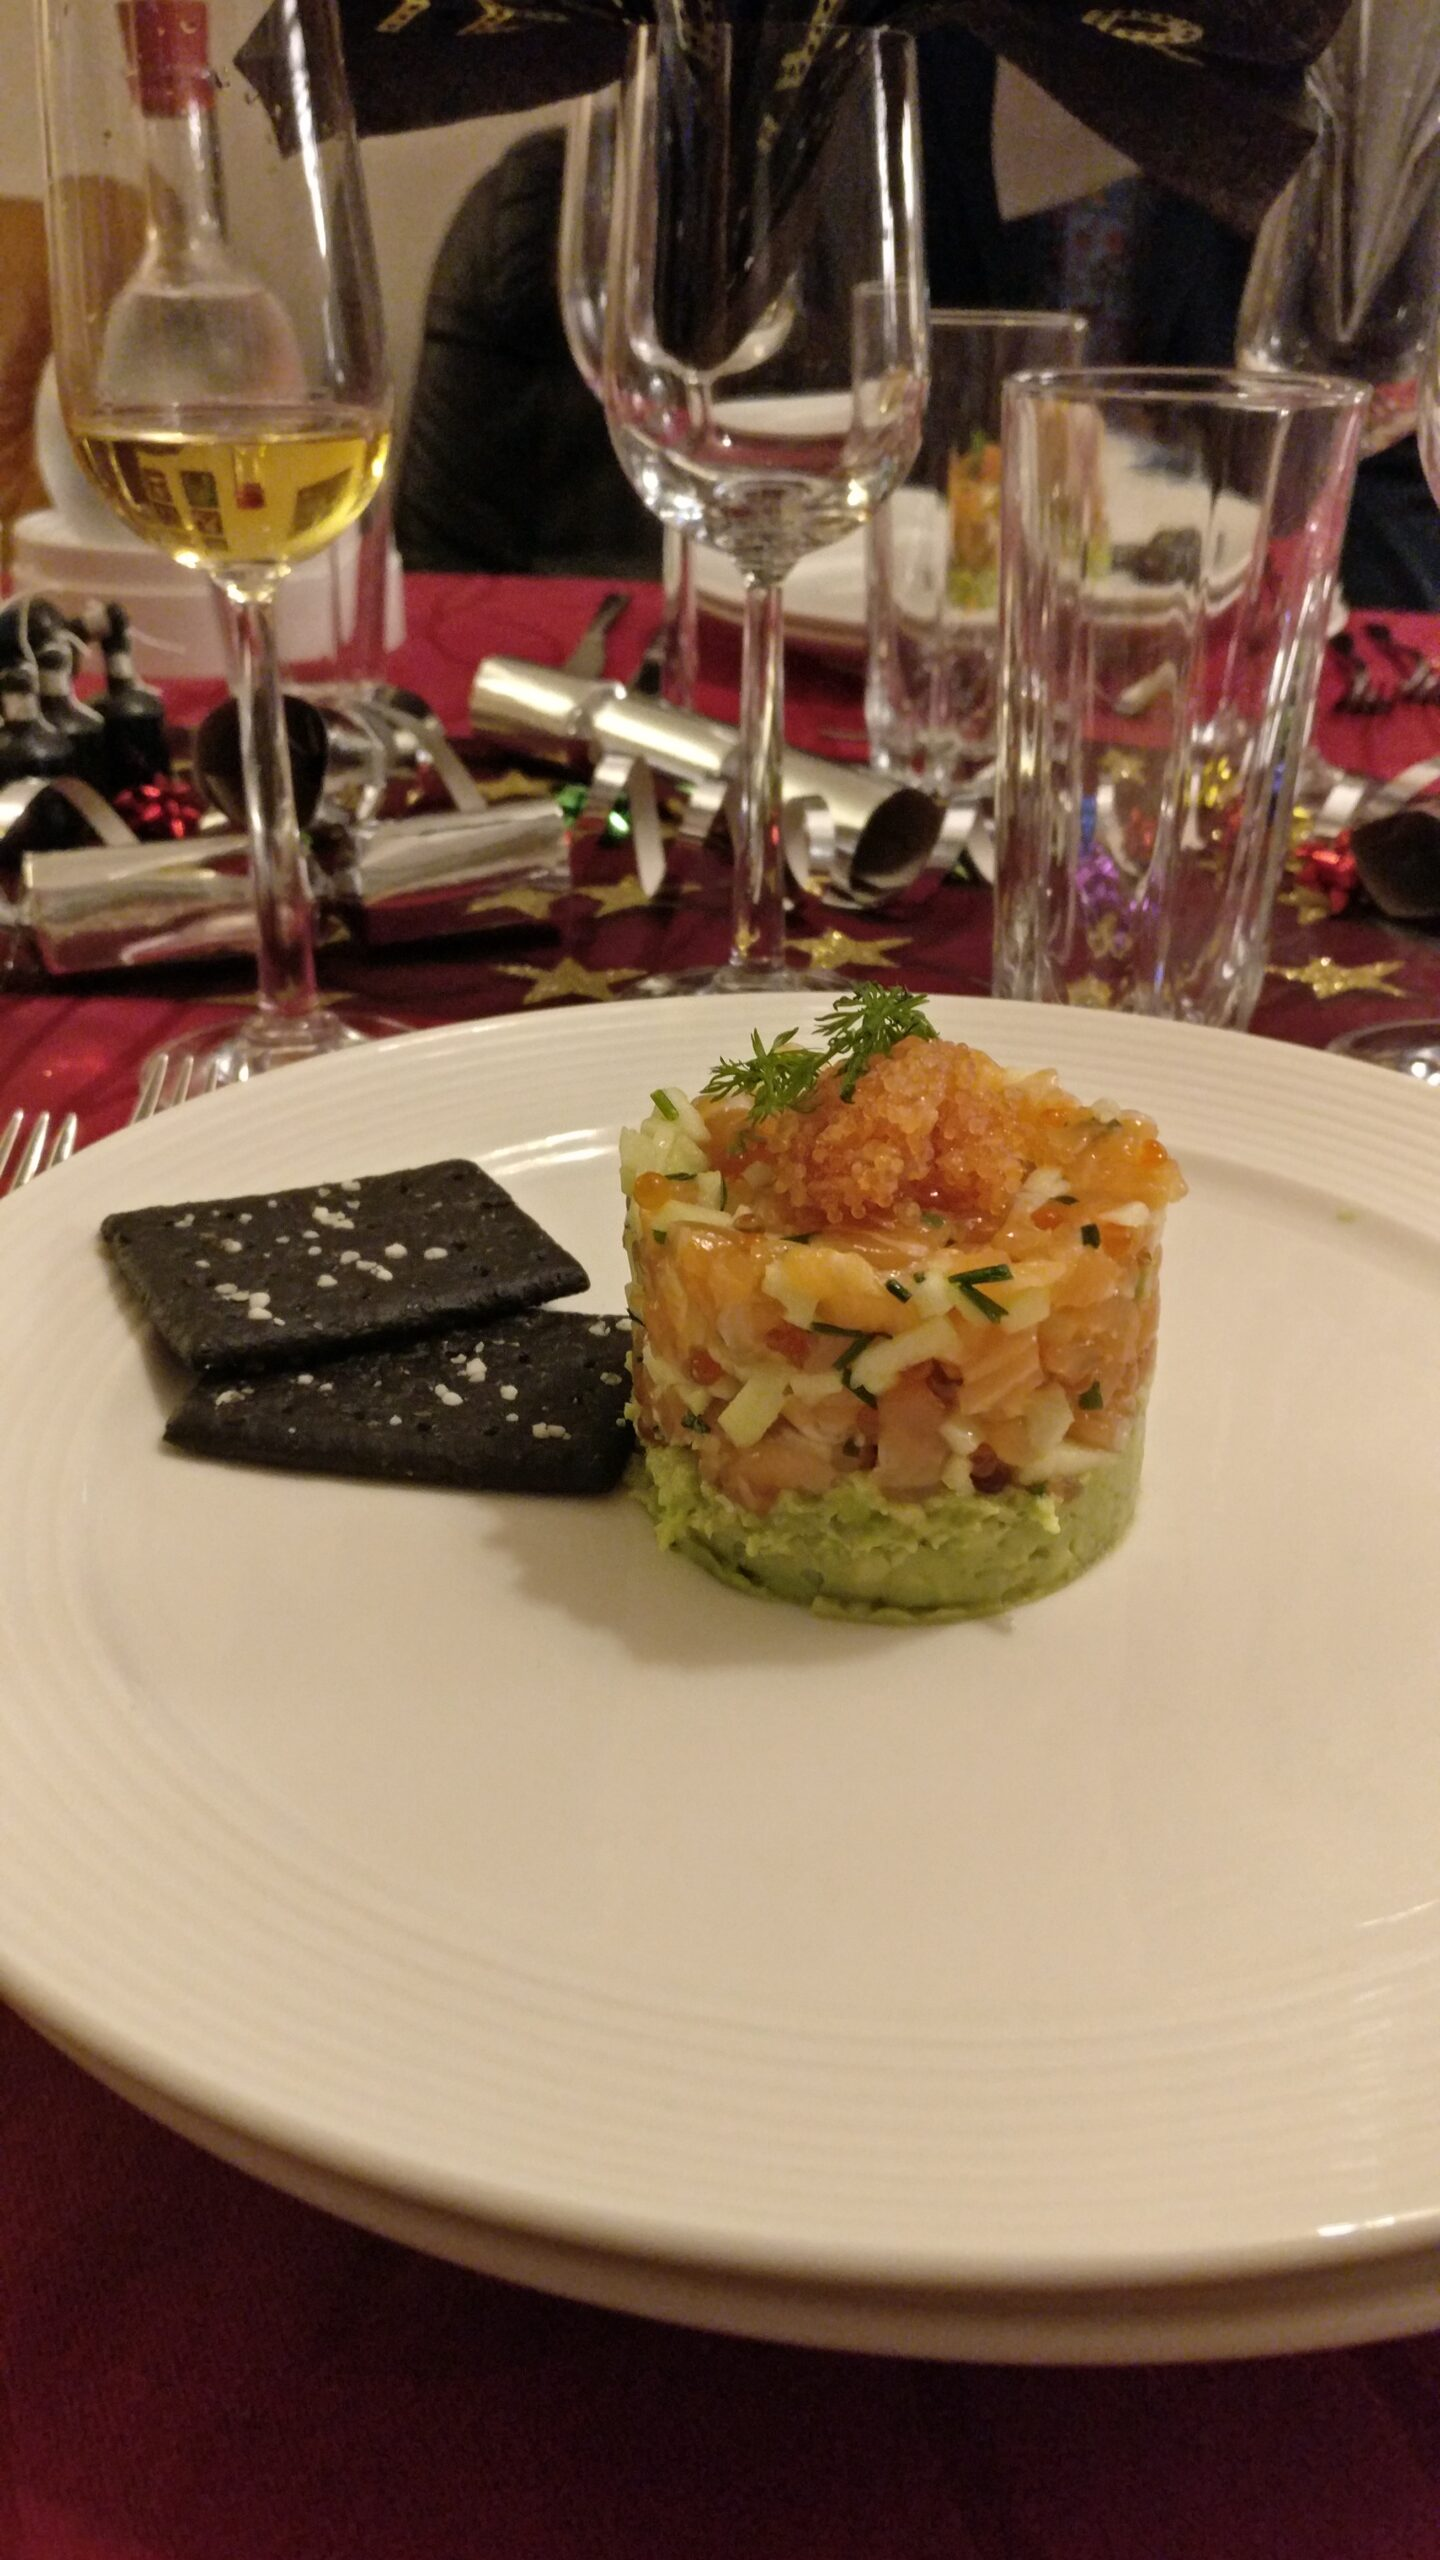
\includegraphics{rmds/images/forret-scaled.jpg}

\hypertarget{uxe6rtefritter}{%
\section{Ærtefritter}\label{uxe6rtefritter}}

Altså ikke fritter som i pommes frites lignende. Men en fritteret
ærtemasse.

Godnatlæsningen i øjeblikket er~The Flavour Thesaurus af Niki Segnit.
Den har tidligere leveret en opskrift der er i fast rotation derhjemme i
nørdborgen. Og nu skal det altså være fritterede ærter.

\hypertarget{forskellige-slags-kartofler}{%
\section{Forskellige slags
kartofler}\label{forskellige-slags-kartofler}}

Vi skal have kartofler til. Men jeg har fået så utroligt mange kogte
kartofler i min barndom at jeg ikke orker at servere dem for nogen,
endnu mindre at skulle spise dem. Så. En oversigt over
standardkartofler. Så her er min liste over forskellige måder at
tilberede kartofler.

Ingen opskrifter. De kommer måske. For de fleste skal der stå ``pommes''
foran.

À la crème Allumette Anglaise Anna Au four Bonne Annè Bouillonkartofler
Brunede kartofler Cannelure Carrées Château Cocotte Copeau Croquette
Dauphine Duchesse Fermiere Fondantes Frites Galettes Gaufrettes Gratin
Gratin (en minute) Hash brown Hasselback Kartoffelmos Kartoffelsouffle
Lorette Lyonnaise Macaire Maître d'hôtel Noisette Paille Parisiennes
Persillees Pont-neuf Purées Faffles Rissollees Rösti Saint-florentin
Sautees Soufflees Spirella

\hypertarget{trykkoger-risotto}{%
\section{Trykkoger risotto}\label{trykkoger-risotto}}

Vi har en trykkoger. Men den bliver ikke brugt så ofte. Det bør der
laves om på, for hele konceptet i trykkogeren er at ting går hurtigt. Og
det har jeg ofte brug for, når alt det andet skal nås.

Min husbond har en hobby, hvor han finder eksotiske opskrifter til mig
på nettet. Det holder mig beskæftiget i køkkenet, så jeg ikke brokker
mig over al den tid der bliver brugt på World of Warcraft. Ren win-win!

Og en af de opskrifter han fandt,handlede om risotto i trykkoger. Så det
prøver vi:

\begin{itemize}
\tightlist
\item
  700 gram champignon
\item
  950 ml kyllingefond
\item
  300 gram risottoris
\item
  3 små løg. Sådan ca. 150 gram i alt. Hakket.
\item
  2 fed hvidløg, finthakket
\item
  1 pakke bacon, skåret i tern.
\item
  1½ dl hvidvin
\item
  Smør, olie, salt, peber og parmasan
\end{itemize}

Baconen blev stegt i trykkogeren. Champignonerne blev renset, skivet og
stegt med baconen. Der blev tilsat en spsk smør og en sjat olie, og
svampene blev stegt til de først havde smidt vandet, og derefter optaget
det igen. Giv dem et godt drys salt. Så kom løgene i, de blev stegt til
de var klare. Hvidløgene blev tilsat og stegte med i et par minutter.
Hvidvin hældt over, og kogt til det ikke duftede af alkohol længere.

Derefter kom risotto risene i. De stegte med til de begyndte at ligne
små isterninger. Lidt gennemsigtige i hjørnerne. Endelig blev fonden
hældt på, og trykkogeren lukket. Fuldt skrald på pladen.

\hypertarget{kandiseret-frugt}{%
\section{Kandiseret frugt}\label{kandiseret-frugt}}

Fra bogen ``Farmacevtens andet Aar i Radio''.

Forbered frugtstykkerne. Druer, æblestykker, appelsin etc.

Fremstil en sukkerlage af 250 sukker, 1 dl vand, 1 tsk eddike og 1 tsk
druesukker. Bring først sukker, druesukker og vand i kog, skum af og
tilsæt eddike. Når lagen er kogt tilstrækkeligt ind - en dråbe af lagen
dryppes i koldt vand - den skal blive sprød som glas.

Dyp hurtigt frugten i lagen og læg dem til tørre på et fad - smurt med
olie eller smør.

\hypertarget{fluxf8dekarameller}{%
\section{Flødekarameller}\label{fluxf8dekarameller}}

Fra bogen ``Farmacevtens andet Aar i Radio''.

\begin{itemize}
\item
  Kog 150 g sukker med 100 g fløde.
\item
  Og 150 g sukker med 25 g smør til karamel.
\end{itemize}

Alt blandes og æltes. Hæld ud på et fladt fad, smurt med smør eller
olie. Lad det stå nogle timer, og udskær i passende firkanter, drys med
flormelis.

\hypertarget{frossen-uxe6bleskum}{%
\section{Frossen æbleskum}\label{frossen-uxe6bleskum}}

\begin{itemize}
\tightlist
\item
  1 kg æbler (gerne med god syre)
\item
  1 bundt citronmelisse
\item
  1 økocitron
\item
  2½ æggehvide (pasteuriseret) Det skulle gerne veje omkring 100 g.
\end{itemize}

\hypertarget{bruxe6ndt-fluxf8de}{%
\section{Brændt fløde}\label{bruxe6ndt-fluxf8de}}

opr fra 27. august 2018

Jeg er rimeligt begejstret for ghee: Klaret smør, hvor proteinerne har
fået lov at brune inden fedtet er hældt fra og sat på køl. Den brunede
valle leverer nogle dybe nøddeagtige smagsnuancer, der giver lidt ekstra
når der steges i smør. Og hvorfor steger vi i klaret smør derhjemme i
stedet for i almindeligt smør? Fordi vallen bruner og brænder og ryger
og udløser røgalarmen. Hælder vi den fra, har vi kun smørfedtet tilbage,
og det kan holde til højere temperaturer end uklaret smør. Det gør det
lettere at få brunet bøffen ordentligt uden at branke den.

Min mand har en hobby med at finde interessante opskrifter, som han så
mener jeg skal lave. Og han faldt over denne her, som basalt set handler
om det samme. I stedet for smør er det bare fløde. Og det er den samme
proces vi ønsker - proteinerne skal gennem en maillardproces og blive
brune. Kemien er lidt avanceret, men den kan fremmes ved at justere på
pH i fløden. Det foreslår Serious Eats at man gør ved hjælp af
bagepulver. Resultatet skulle blive en brun fløde med toner af nødder og
karamel. Det lyder lækkert. Så det skal prøves.

Der er to grundlæggende veje. Sous vide og trykkogeren.

Først sous vide:

Det var ikke helt let at få fløde i plastikposen. Jeg blandede en halv
liter piskefløde med en kvart teske bagepulver, og smed det i fryseren i
mindre portioner. Derefter var det ret let. Vandbadet blev varmet op til
82 grader, og så røg poserne i vandet i 24 timer.

Indholdet var pænt lysebrunt. Hvad det også var, var skilt. Den nu
brændte fløde kom i gryden sammen med æggeblommer, sukker og vanille -
søg efter min standard vanilleis opskrift hvis du vil have detaljerne.

Alternativet var trykkogeren.

Igen blev en halv liter fløde blandet med en kvart teske bagepulver.
Fløden blev derefter hældt på henkogningsglas, der kom i trykkogeren ved
den høje temperatur i to timer. Efter glassene var kølet så meget af at
jeg kunne håndtere dem, blev der lavet is af dem.

Farven på fløden var mere brun.

Og det færdige resultat? Isen baseret på den sous videde fløde var
hårdere end den baseret på den trykkogte. Men smagen var ca. den samme.
Måske lidt anderledes, men det kunne lige så godt skyldes den anderledes
mundoplevelse fordi den smeltede anderledes. Hvad det egentlig skyldes
er et godt spørgsmål, men det må næsten skyldes at fløden skilte
undervejs.

Konklusionen er derfor, at trykkogt fløde er ret godt. Lækre nuancer af
nødder, lidt mørk chokolade og karamel. Men der er ingen grund til at
have et vandbad til at stå og bruge strøm i 24 timer, hvis det kan
klares på to timer i en trykkoger.

\hypertarget{barbecuesovs}{%
\section{Barbecuesovs}\label{barbecuesovs}}

Oprindeligt publiceret 27. august 2015

Vi skal have pulled pork i aften. Der har ligget en og hygget sig i
fryseren i et stykke tid, og nu er den tøet op. Det bliver serveret som
byg-selv-burgere, så opskriften er ret enkel i dag. Der trænger nemlig
til at blive ryddet op, så der er andet at se til end at så i køkkenet
hele dagen:

\begin{itemize}
\tightlist
\item
  1 pulled pork
\item
  Burgerboller
\item
  1 portion coleslaw fra Føtex
\item
  Mayonaise
\item
  Barbecuesovs
\end{itemize}

Den langtrukne gris varmes (overhældt med en smule bouillon), coleslawen
røres sammen og burgerbollerne varmes. Det hele stilles på bordet med
mayo og barbecuesovs.~

Helt simpelt, men det er for let.

Barbecuesovsen bliver derfor hjemmerørt:

\begin{itemize}
\tightlist
\item
  2 dl ketchup
\item
  150 g mørk muscovadosukker
\item
  4 spsk æblecidereddike
\item
  4 tsk soya
\item
  4 tsk sennep
\item
  4 tsk røget paprika
\item
  2 tsk chili
\item
  Et par drys allehånde, kardemomme og ingefær
\item
  2 spsk vand
\end{itemize}

Det hele smides i en gryde og bringes i kog. Og sættes derefter på køl.

Mayoen bliver ikke helt hjemmelavet, men købeudgaven bliver justeret
lidt.

\begin{itemize}
\tightlist
\item
  3 dl mayonaise
\item
  1 tsk worchester sauce
\item
  1 tsk stærk sennep
\item
  Et nip salt
\end{itemize}

Og så tager jeg en håndfuld bagekartofler, skærer dem i stænger, og
steger dem i (rigeligt) smør på panden til de er gyldne og møre.

\hypertarget{hollandaise-sifon}{%
\section{Hollandaise sifon}\label{hollandaise-sifon}}

Ikke afprøvet, så på eget ansvar!~

Ingredienslisten er fra Brødrene Prices grund-hollandaise:

\begin{itemize}
\tightlist
\item
  250 g smør
\item
  3 æggeblommer
\item
  Saft af ½ citron
\item
  En skefuld fiskefond
\item
  Salt og hvid peber
\end{itemize}

Personligt ville jeg nok skalere op til fire æggeblommer. Så skal der
bruges 333 gram smør, en sqeeze citron ekstra, og en teskefuld fiskefond
mere. Men det er mest fordi jeg er bange for upasteuriserede æg, og
fordi de pasteuriserede æggeblommer kommer i bægre af to styk. Og det
der med at måle halvdelen af et bæger æggeblommer gider jeg ikke.
Fremgangsmåde:

Klar smørret.~ Pisk æggeblommerne med fonden, og derefter (LANGSOMT!)
det klarede smør i blommerne på vandbad. Smag til med citron, salt og
peber.~ Hæld hele blandingen på en ½ liters sifon, giv den et enkelt
skud lattergas, og lad den stå en times tid i varmt (max 65 grader)
vand.

Og forvent nu ikke at det kommer ud som en normal hollandaise, det er en
skum vi laver her. Hollandaisen passer godt til fisk, men går også an
til kylling.

Eftersom Hollandaisen er en af modersovsene, og basalt set grundlaget
for Bearnaisen, vil det formentlig være et udemærket alternativ til den
opskrift jeg tidligere har bragt på netop Bearnaise på sifon.

\hypertarget{fruit-dumplings.-boulette-klimp.-eller-noget}{%
\section{Fruit dumplings. Boulette, klimp. Eller
noget}\label{fruit-dumplings.-boulette-klimp.-eller-noget}}

Opr. fra 11. marts 2018

Hvad det hedder på dansk aner jeg ikke. Men på tjekkisk hedder det
ovocné knedlíky. En sød dej, omkring noget frugt. Og så kogt. Det er
underligt, men typisk tjekkisk.

NB: Denne opskrift er en jeg har haft med hjem fra Prag. Den trænger til
at blive justeret, for der er noget galt. Den skal have noget mindre
mælk for at være til at arbejde med. Jeg prøvede den her i weekenden, og
der var løsningen at give den mere mel. Det bliver de mindre søde af, så
næste gang er det mælken der justeres med.

\begin{itemize}
\tightlist
\item
  15 g gær
\item
  40 gram sukker
\item
  1 nip salt
\item
  250 g mel
\item
  1 æg
\item
  250 ml mælk
\item
  8 gram vanillesukker
\item
  20 blommer, abrikoser, jordbær eller anden frugt
\item
  200 g smør
\item
  150 g flormelis
\end{itemize}

Gær, sukker og salt røres sammen, og blandes med mel, æg, mælk og
vanillesukker. Der æltes. Lad dejen hæve i 45 minutter. Rul den ud og
skær den ud i 20 firkantede stykker.

Rens frugten, fjern sten hvis der er nogen. Pak frugten ind i dejen (gør
dine hænder våde først, så går det lettere), og lad dem hæve yderligere
5-6 minutter.

Kog dem i rigelige mængder saltet vand i 8-10 minutter. Lad være med at
komme for mange i vandet ad gangen. Ikke mere end en fem stykker.

Smelt smørret og hæld det over, og drys endelig med flormelis.

Man kan måske med fordel spare lidt på smørret, men klassisk tjekkiske
opskrifter er designet efter at du skal have kalorier nok til at brydes
i 5 meter dyb sne med en bjørn inden du skal ud og fælde en skov.

\hypertarget{buffalo-crunch}{%
\section{Buffalo-crunch}\label{buffalo-crunch}}

Insekter skal der til!

Et lille knas til det søde køkken. * 100 gram frysetørrede buffalo-orme
* 4 spsk sukker * evt. et krydderi. Ingefær, anisfrø eller lignende,
efter hvad der passer med hvad de skal serveres til.

Varm sukkeret op på en pande med en sjat vand. Rør rundt og
karamelliser.

Tilsæt ormene sammen med krydderiet, og rør videre. Når ormene er dækket
af karamel, overføres de til bagepapir, og skilles ad med et par gafler.

Brug dem til anretning af desserter, brownies, is-anretninger o.lign.

\hypertarget{mit-surdejsbruxf8d}{%
\section{Mit surdejsbrød}\label{mit-surdejsbruxf8d}}

fra 20. april 2020

\hypertarget{surdejsrester}{%
\section{Surdejsrester}\label{surdejsrester}}

Bent, vores surdej, er stadig ikke så livlig som de surdeje jeg ser på
nettet. Men han er livlig nok, og selv efter en uge i køleskabet, skal
han ikke fodres ret meget for at levere et glimrende brød. Altså bortset
fra at jeg glemte at komme salt nok i. Altid veje salt!

Men hvad med resterne? Hver gang han fodres, hælder jeg det meste af ham
i vasken. Ellers ender vi med helt enorme mængder Bent.

Lad os prøve at lave knækbrød.

250 g Bent (eller hvad du nu kalder din surdej) 125 g mel 60 g smør ½
tsk salt Tørrede krydderurter, olie og groft salt

Ælt Bent, mel, salt og smør sammen. Del dejen i to, og form dem til
firkantede plader. Sæt dem på køl en halv time.

Rul hver af pladerne ud til ca. 1½ mm tykkelse, smør dem med olie, og
drys salt og krydderurter ud over dem. Timian er godt! Skær dem ud i
passende stykker. Vi har et pizzahjul der tages i anvendelse.

Prik alle stykkerne med en gaffel. Eller en prikrulle, som jeg var så
heldig at få til jul.

Bag dem ved 180 grader i 20 til 25 minutter. Eller til de begynder at
blive brune i kanterne. Vend gerne pladen efter 10 minutter, hvis din
ovn (som vores) ikke giver helt jævn varme.

Køl af på bagerist - det går hurtigere, og de bliver sprødere når der er
fri passage af luft omkring dem.

\hypertarget{simpel-mad-2}{%
\section{Simpel mad 2}\label{simpel-mad-2}}

opr fra 3. februar 2012

Det skal være let. Meget let. For klokken er som regel 17.30 når jeg
kommer hjem. Kæresten har fri kl. 17, og er hjemme kl. 18. Og det er når
indkøbslisten er i bund, og der ikke skal købes ind. Så maden skal være
let, hurtig, og ikke kræve for meget. Og samtidig må den godt være god.
Den letteste måde at skære ned på tiden er at bruge få ingredienser.~

Denne opskrift har vi ikke prøvet endnu, men det ser godt ud. Den er
ikke selvkomponeret, og med fem ingredienser er den mere end dobbelt så
kompliceret som~peberfrugtkyllingen. Men den er stadig enkel at gå til.
Opskriften er tyvstjålet fra~Travel Through Food.

500 g kyllingelår, uden skind og ben, skåret i 2-3 skiver (hver) 5-6 fed
hakket hvidløg 1½ tsk tørret persille (her ville jeg være fristet af
frisk, men det kræver at vi får sat gang i et andet projekt) 1 spsk mel
1½ spsk olivenolie~ Salt og peber

Alt, bortset fra melet og olie, blandes sammen, og får lov at trække i
et kvarter. Tilsæt mel, og rod godt rundt. Varm olien i en pande, steg
kyllingerne til de er gyldne. De skal have 2-3 minutter på hver side,
afhængig af tykkelse og varme. Server.

\hypertarget{mit-surdejsbruxf8d-1}{%
\section{Mit surdejsbrød}\label{mit-surdejsbruxf8d-1}}

oprindelig fra 20. april 2020

Danmark blev ramt af Corana-virusen. Eller Wuhan-influenzaen. Eller
Covid-19. Eller hvad vi nu kalder den. Vi gik i lockdown. Næsten. Og jeg
kom i kontakt med min indre Finne.

Fredag den 13. marts 2020 blev min lille surdej undfanget. Og her lidt
over en måned senere, spytter den et nyt brød ud hver anden dag. For det
smager godt, og derfor holder det ikke så længe.

Hvordan blev surdejen lavet?

2 dl mel blev rørt sammen med 2 dl vand, og efterladt i en plastbøtte på
køkkenbordet. Låget lå løst på - så tabte hvidløg ikke endte i dejen,
men ikke fast. Det er diverse bakterier og gærceller fra luften vi skal
have ned i blandingen, så den kan gære.

Da det begyndte at boble, hældte jeg det meste fra, tilsatte 1½ dl mel
og 1½ dl vand, og rørte rundt.

Efter en uges tid tog jeg det jeg ellers ville have hældt i afløbet, og
hældte det i en skål. Den fik et par dl mel og tilsvarende vand, der
blev rørt rundt. Og så ventede jeg et par timer, gav den 450 gram mel,
og 3½ dl vand. Samt en teske salt. Der blev rørt rundt, og efter at
blandingen havde stået på køkkenbordet et par timer, kom den i
køleskabet natten over. Undervejs blev dejen foldet ind over sig selv en
4-5 gange. Dejen blev fordelt i klatter og smidt i ovnen.

Og det var virkelig ikke særlig heldigt. Det blev spist, men kun fordi
jeg har giftet mig med en jyde der ikke bryder sig om at smide mad ud.

Derefter fortsatte jeg med at fodre dejen. Den fik undervejs vist en
pakke gær, og fik besked om at hvis ikke den tog sig sammen, ville den
blive hældt ud.

Efter yderligere en uge prøvede jeg igen. Lidt enklere denne gang.
Overskydende surdej ud i skål, mel og vand. Vent en 3-4 timer til det
bobler. 450 gram mel, 3½ dl vand, et par teskefulde sukker, en toppet
teske salt, rør, henstil på køkkenbordet 12 timer, hældes i en stegeso
(der har stået inde i ovnen mens den blev varmet op til 250 grader), låg
på, ind i ovn, vent 20 minutter, låg af, temperatur ned på 200 grader,
vent yderligere 15-20 minutter. Og vupti:

Jeg er blevet medlem af en surdejsgruppe på Facebook. Og de går meget
videnskabeligt til værks. Det her dækker fint behovet, og vi kan nu
klare os gennem en alvorlig gærkrise, alene ved hjælp af vores lille
surdej.

Der stadig ikke har fået et navn.

\hypertarget{molekyluxe6r-gastronomi}{%
\section{Molekylær gastronomi}\label{molekyluxe6r-gastronomi}}

Oprindeligt fra 20. juli 2011

Eller rettere, molekylær kogekunst, er en af de ting der hygges med
derhjemme i køkkenet. Det kan være svært at forklare hvorfor det har
stor nørdværdi og er sjovt at bage chololadekage ved hjælp af en sifon
og lattergas, så det vil jeg ikke prøve. Blot konstatere, at jeg synes
det er besværet værd, og så kompenserer det for at jeg ikke har et
rigtigt kemisk laboratorium at arbejde i.

Endelig er den slags en nødvendig del af arsenalet, når man ligger i
køkkenkrig med lillebror, og han har adgang til flydende nitrogen.

Inspirationen kommer som regel fra denne blog: khymos.org, eller
rettere, den samling af opskrifter manden bag, Martin Lersch, har lagt
på nettet. Den kan hentes her. Det kan være vanskeligt at finde
ingredienserne, men Inco forhandler Texturas-serien. Det kræver at man
har et Inco-kort, så det har vi derhjemme

\hypertarget{suxe5dan-er-det-nuxe6sten-dagens-kuxf8kkenprojekt}{%
\section{Sådan er det næsten -- dagens
køkkenprojekt}\label{suxe5dan-er-det-nuxe6sten-dagens-kuxf8kkenprojekt}}

oprindeligt far 3. april 2012

Kæresten har fødselsdag. Om en måneds tid, men fordi det der med at være
ude i sidste øjeblik tilsyneladende er arveligt, er det nødvendigt at gå
i gang med at punke for dato, ønskeliste, invitationer og ønsker til
menuen i rigtig god tid. Jeg har været i gang de sidste to måneder, og
nu begynder de fleste ting at falde på plads. Vi fik godt nok udvidet
projektet for 1½ uge siden. Svogeren in spe, Martin, har fødselsdag ca.
samtidig, og de plejer at holde fødselsdag sammen. Nu bor hele
svigermekanikken i Jylland, så den fælles fødselsdag skal holdes i
Rødovre. Det er et større logistisk projekt. Og jeg skal lave maden.
Hvilket i sig selv er lidt af en udfordring, af to årsager. Dels er
lejligheden ikke helt stor nok til 12 personer, det gælder både stuen og
køkkenet. Dels er der visse forventninger.

Af uransalige årsager er jeg udråbt som den store mesterkok. Det er
måske ikke så mystisk alligevel. Men det lægger et vist
forventningspres. Også fordi jeg ligger i krig med lillebror, og han
sætter nok et nyt niveau for kogekunst her på søndag.

Jeg føler det lidt ligesom Jason Ogg fra Discworld serien. Han er en
rigtig god smed, han kan sætte sko på alt. Men det har en pris:

``He could shoe anything, could Jason Ogg. They'd brought him an ant
once, for a joke, and he'd sat up all night with a magnifying glass and
an anvil made out of the head of a pin. The any was still around,
somewhere--sometimes he could hear it clatter across the floor. \ldots{}

But that was the bargain--you shod anything they brought to you,
anything, and the payment was that you could shoe anything. There had
always been a smith in Lancre, and everyone knew the smith in Lancre was
a very powerful smith indeed.'

Så denne dag i påskeferien bruges på at øve mig på at lave rillettes.
Når jeg har fundet ud af hvordan jeg let får billeder på denne blog,
kommer der en mere udførlig beretning.

\hypertarget{noget-med-majs-juice}{%
\section{Noget med majs juice}\label{noget-med-majs-juice}}

Uvist hvorfor mener (dele af) svigerfamilien, at jeg er den store
bagermester. Det har man for at bage boller til dem en enkelt gang.

Men så må der hellere leves op til det. Næste bageprojekt bliver efter
denne opskrift:

190 g æg 20 g æggeblommer 80 g sukker 1,5 g salt 75 g majs juice 40 g
smeltet smør 30 g mel

Æggene, i deres respektive inkarnationer piskes sammen, resten af
ingredienserne tilsættes og piskes.

Blandingen sis og hældes på en flødeskumssifon, og der skydes to doser
lattergas på.

Der sprøjtes dej ud i 2½ dl beholder (plast), den sættes i mikroovnen
ved 900 W i 40 sekunder. Gentag til al dej er brugt.

Opskriften kommer fra ``Texture'', der kan downloades på den norske
molekylær gastronomiske blog Khymos.org.

\hypertarget{karamel-uxe6bler}{%
\section{Karamel æbler}\label{karamel-uxe6bler}}

En opskrift fra det gamle DDR. Hentet på DDR museet i Berlin. Og de
havde den fra ``Kuchen, Torten und Gebäck'' fra 1971. Udgivet på
``Verlag für die Frau''. Jeg ved ikke om det i dag betragtes som meget
misogynt, eller meget progressivt, at der var et forlag for kvinder.

Anyway:

60 g sukker 2 spsk honning næsten 250 ml vand saften af en citron 4
store madæbler 120 g mel 2 spsk sukker 1 nip salt 2 æg Olie Flormelis.

80 g sukker, honning, 125 ml vand, og citronsaft blandes, og koges ind
til en halvtyk sirup. Skræl æblerne, og skær i kvarte - læg dem i
siruppen.

Tag kaserollen af varmen, og lad den stå i 1 time - vend æblerne
regelmæssigt.

Imens sigtes melet med salt, og blandes med 2 spsk sukker samt
æggeblommerne. Tilføj 125 ml vand, og rør sammen.

Pisk æggehviderne, og fold dem ind i dejen.

Fjern æblerne fra siruppen, og lad dem dryppe lidt af. Dyp dem i dejen,
og kog dem i olien til de er brune og sprøde. Lad dem dryppe af på
fedtsugende papir, og drys med flormelis.

\hypertarget{kage-i-ramekiner}{%
\section{Kage i ramekiner}\label{kage-i-ramekiner}}

Fra dengang dette var en hjemmeside - 21. marts 2012

Fra loggen. Ja, det er noget folk søger på, og finder denne side. Man
fatter det ikke

En ramekin er en lille glaceret procelænsskål. De er ret fikse til Crème
brûléel og andre ting. Herhjemme bliver de mest brugt til servering, men
det er fordi det med kager og den slags ikke er noget vi gør så meget
i.~

Et sted hvor de kan bruges, men egentlig ikke er så velegnet, er i min
chokolade sifon mikroovnskage. Og ellers: Hiv fat i din foretrukne
cupcake opskrift (den findes i de fleste kogebøger under navnet
``muffins'', og hæld den i en ramekin. Evt. foret med en almindelig
muffinform i papir. Hvis ikke der kommer papirform i, så smør grundigt
med (rigeligt!) smør, så kagen slipper formen. Det giver fine lige
kanter på kagen. Her er et eksempel på en muffinopskrift. Den er ikke
specielt beregnet på ramekiner, men det er ikke noget problem.

ca. 250 g hvedemel -- føl dig frem, det kommer an på æggets størrelse. 2
1/2 dl mælk. Kærnemælk giver lige et ekstra pift, så brug det om muligt
30 g smør 1 æg 2 tsk bagepulver 50 g sukker Chokolade eller bær. Eller
begge dele. Ca. 125 g grovhakket chokolade passer, men her må man også
føle sig lidt frem, eksempelvis efter bærrenes størrelse.

Smelt smørret, bland det med mælk og æg, og rør sukker, bagepulver og
mel i. Gem lidt af melet og drys det over chokoladen eller bærrene, så
fordeler de sig bedre i dejen. Hæld dejen i muffinforme (eller
ramekiner), og bag dem ved 225 grader i ca. 20 minutter -- her skal du
også føle dig lidt frem, ovne har personlighed, og det er ikke alle der
rammer præcis 225 grader selvom man har indstillet dem til det. Husk at
smøre formene rigtig grundigt hvis du ikke smider en papirform i også!
Det kan ikke gentages ofte nok.

Når de er kølet lidt af kan man lave cupcakes ud af dem. Det gør man ved
at hælde noget glasur og krymmel i suspekte farver ud over dem, og
derefter hævde at de er meget finere og mere moderigtige end muffins.
Man kan også bare, helt oldschool, droppe neonfarverne og kalde dem for
muffins.~

Man kan hælde så megen anden kagedej i dem. Og teknisk set er ramekiner
ikke kun de små skåle, de hedder ramekiner op til i hvert fald en kvart
liter. Så der er rigeligt med muligheder. Men for at være helt ærlig?
Ramekiner bidrager med to ting: Din kage får en pæn rund facon, og så
mangedobler du størrelsen af opvasken. Skal kagen være pænt rund, så
brug en springform i stedet. Det er næste håbløst at få kagerne ud af en
ramekin, jeg har prøvet\ldots{} Skal det absolut være, så gå efter en
teflonforet sag, og anskaf en opvaskemaskine.

\hypertarget{uxe6bletuxe6rte}{%
\section{Æbletærte}\label{uxe6bletuxe6rte}}

I julegave fik jeg af husbonden en kombineret
æbleskræller/udhuser/slicer. Sådan en fætter her:

Eller, i følge manualen, en æblemaskine. Jeg fik også en prikruller. Og
en kogebog med opskrifter på tærter.

Jeg kan godt forstå et vink med en vognstang. Så jeg måtte hellere komme
igang.

Tærtedej - bare den fra supermarkedet, rulles ud (af posen) og prikkes
med prikrulleren. Den fordele i tærteformen.

Et par æbler skrælles, kernehuset fjernes, og slices. Altsammen i en
omgang på æblemaskinen. De fordeles i tærteformen, og må godt rage pænt
over kanten. 1½ spsk maizena, 1 tsk kanel og 1½ dl sukker blandes. Det
meste drysses over æblerne.

Yderligere tærtedej prikkes, og monteres over tærten. Kanterne forsegles
og resten af kanel/sukker blandingen drysses ud over.

Bages i 35 minutter ved 190 grader. Sænk temperaturen til 160 grader og
bag i yderligere 25 minutter.

\hypertarget{uxe6bletuxe6rte-og-det-er-en-anden-end-uxe6bletuxe6rte}{%
\section{Æbletærte og det er en anden end
æbletærte}\label{uxe6bletuxe6rte-og-det-er-en-anden-end-uxe6bletuxe6rte}}

250 gram mørdej/tærtedej - bare en rulle fra supermarkedet

4 store æbler

50 gram smør

75 gram muscovadosukker (eller brun farin. Eller bare almindeligt
sukker, hvis du virkelig ikke har andet)

1 spsk kanel

placer dejen i smurt springform, forbag i 10 minutter ved 170 grader.

Skræl æblerne, skær dem ud i grove chunks, og vend dem i kanel.

Smelt smørret på en pande ved svag varme. Tilsæt sukker når det bobler,
og når sukkeret også er smeltet, så tilsæt æblerne, og lad dem hygge sig
i karamelblandingen et par minutter. Hæld æbleblandingen i tærten - få
al karamel med! og bag den i ca. 20 minutter (eller til den har fået
lidt farve) ved 175 grader.

Giv en klat flødeskum, creme fraiche eller vanilleis til.

\hypertarget{fisk-puxe5-finsk}{%
\section{fisk på finsk}\label{fisk-puxe5-finsk}}

Vi tror nok det er ``a'la Mannerheim''. Steg fisk, lejret på et par nye
kartofler (skåret så der er flader at lægge fisken på). Stegt gulerød
eller lignende. Og kanteralsovs.

Piskede æggehvider revet citronskal makroner. Dessert bestilling.

\hypertarget{ting-fra-weekendavisen}{%
\section{Ting fra weekendavisen}\label{ting-fra-weekendavisen}}

https://www.weekendavisen.dk/kultur/pasta-a-la-tiktok
https://www.weekendavisen.dk/kultur/spis-paris
https://www.weekendavisen.dk/kultur/maizena-alkymi
https://www.weekendavisen.dk/kultur/kunsten-at-klare-kikaerterne
https://www.weekendavisen.dk/kultur/saucernes-laerling
https://www.weekendavisen.dk/kultur/sodavand
https://www.weekendavisen.dk/kultur/aeggekogeriet
https://www.weekendavisen.dk/kultur/ben-med-et-hul
https://www.weekendavisen.dk/kultur/honninghjertets-forbandelse
https://www.weekendavisen.dk/kultur/creme

Poached Pear Wrapped in Brie, Baked in Puff Pastry 💫 From the outside,
it's golden and glossy. Inside? Creamy brie and a glistening red wine
pear. This is dessert-meets-cheese course in the most spectacular way.
🛒 Ingredients For the Poached Pear 1 firm pear, peeled and cored from
the bottom 200 ml red wine 2 tbsp brown sugar 1 cinnamon stick 2 cloves
Zest of ½ orange Optional: splash of balsamic vinegar For the Burrata
Bomb 1 wheel of brie or camembert (200--250 g) 1 sheet of puff pastry
(thawed) 1 egg, beaten (for egg wash) Optional: pinch of flaky salt or
rosemary 🍽️ Instructions The pear is deeply infused with wine and spice.
The cheese softens to ooze. The pastry bakes to golden crunch.
Together---they become a showstopping centerpiece. 🍷 Poach the Pear:
Combine red wine, sugar, cinnamon, cloves, zest, and vinegar in a
saucepan. Add pear and simmer gently for 20--25 minutes until ruby red
and tender. Let cool in the liquid. 🧀 Assemble the Center: Carefully
slice the brie in half horizontally. Place the drained pear upright in
the center of the bottom half. Place the top half back over, gently
pressing around the pear to seal. 🧈 Wrap in Puff Pastry: Roll out puff
pastry and wrap the stuffed cheese completely, trimming and sealing
edges underneath. Place seam-side down on parchment. 🥚 Egg Wash \&
Bake: Brush pastry with beaten egg. Optional: sprinkle flaky salt or
herbs. Bake at 200°C (392°F) for 20--25 minutes until deeply golden. Let
rest 5 minutes. 🔪 Reveal the Pearl: Slice through the crust tableside
for the full effect---molten cheese, rich pear, and crackling pastry in
one elegant cut. 📋 Recipe Details Prep Time: 30 minutes Cook Time: 25
minutes Resting Time: 10 minutes Servings: 4

\hypertarget{fler-noter}{%
\section{fler noter}\label{fler-noter}}

\hypertarget{tuxe6rte-med-stegte-svampe-og-guleruxf8dder---brunet-smuxf8r-sifon}{%
\section{Tærte med stegte svampe og gulerødder - brunet smør
sifon}\label{tuxe6rte-med-stegte-svampe-og-guleruxf8dder---brunet-smuxf8r-sifon}}

4 portioner

Tærte: * 120 g hvedemel * 48 g hvidvin * 24 g smeltet smør * 10 g sukker
* 6 g fint salt

Sifon: * 76 g æggehvider * 58 g æggeblommer * 3.2 g fint salt * 3.2 g
hvidvinseddike * 3.2 g dijonsennep * 180 g brunet smør - ca. 90 grader c

Stegte grøntsager * 3.2 små skrubbede gulerødder * 80 g champignon i
skiver * 60 g østershat i strimler * 690 g bøgehatte * brunet smør til
stegning * salt * peber

Tærte: Ælt alle ingredienser hurtigt sammen og rul dejen tyndt ud. Stik
den ud og kom i tærte forme. Bag tærterne i pres mellem to forme - til
de er sprøde og gyldne. 10 - 12 minutter ved 180 grader c.

Sifon: Blend æggehvider, blommer, salt, eddike og sennep. Tilsæt brunet
smør i tynd stråle mens blenderen kører. Kom den i sifon, tilsæt en
patron og ryst flasken grundigt. Hold den varm til servering.

Grøntsager: Blancher gulerødder i saltet vand. Steg svampene i brunet
smør og tilsæt gulerødder. Anret grøntsager i de små tærter. Sifoner
over - pynt med en urt.

\bookmarksetup{startatroot}

\hypertarget{lidt-mere-teoretisk}{%
\chapter{Lidt mere teoretisk}\label{lidt-mere-teoretisk}}

\hypertarget{sifon-forsuxf8g}{%
\section{Sifon forsøg}\label{sifon-forsuxf8g}}

Et rygte løber. En hurtig måde at trække smag ud af ting, og ind i
alkohol, skulle være at bruge en sifon. Fremgangsmåden skulle være:

Tag nogle halve jordbær, og hæld dem i sifonen. Hæld neutral vodka oven
i. Skru låget på, giv den et skud lattergas, ryst, vent et par minutter.
Udløs trykket og si jordbærrene fra. Og så skulle vodkaen smage temmelig
meget af jordbær. Mere end hvis de bare havde ligget i vodkaen. Om det
virker, aner jeg ikke. Men det skal testes.

\hypertarget{sifontip}{%
\section{Sifontip}\label{sifontip}}

Ikke en egentlig opskrift, men et lille trick man kan lave med en sifon.

Pil kernerne ud af et granatæble, og hæld dem i sifonen. Giv sifonen et
skud CO2, ikke den lattergas man normalt bruger til flødeskum og de
fleste andre sifonopskrifter.~ Stil sifonen i køleskab et par timer, og
brug kernerne som drys på isen eller i salaten. De prikker nu med
kulsyre.

Ikke noget stort trick, men et lille fif til at løfte de i forvejen
lækre granatæblekerner. Lad CO2 patronen blive siddende på. Ideen er at
skabe så højt CO2-tryk i sifonen som det nu kan lade sig gøre, så
kernerne optager kulsyren.

\hypertarget{svampe}{%
\section{Svampe}\label{svampe}}

Noget af det magiske ved svampe er deres indhold af frie aminosyrer.
Især glutaminsyre. Når den nedbrydes under tilberedningen, får vi på
helt naturlig vis mononatriumglutamat, eller det utroligt farlige MSG
som veganere og andre med forkærlighed for svampe er meget bange for.
Nej, jeg forstår heller ikke logikken.

Anyway, MSG fra svampe er koncentreret umami, særlig mundfylde - og så
forstærker det ca. alle andre smage.

Det viser sig i forskningen at glutamats smag mere end fordobles, hvis
det kombineres med visse nukleinsyrer - og netop tørrede svampe har en
høj koncentration af nukleinsyren guanylat. Og så er der fuld skrue på
umamismagen.

Svampe er ikke grøntsager:


\includegraphics{rmds/images/svampe.png}

Men de har især særligt stærke cellevægge. De indeholder kitin, der ikke
er vandopløseligt, i modsætning til planters cellevægge, der bruger
pektin i samme rolle.

Det betyder at svampene bevarer (mere) af deres struktur ved
tilberedning. Det er endnu en af årsagerne til at de minder en del om
kød i både smag og tekstur.

Store dele af forskellene mellem de forskellige spisesvampe er knyttet
til duftstofferne. Octenol giver noter af skovbund, men noterne spænder
fra mandler til skaldyr.

For de fleste svampe gælder det at deres aromastoffer intensiveres når
de tørres.

En frisk svamp indeholder ca 80\% vand. Det skal reduceres ved
tilberedningen, og det gøres bedst ved moderat varme i længere tid,
gerne tørstegning, så vandet fordamper letere. Når vandet er delvist
fordampet, har vi fået aktiveret aminosyrer, nukleinsyrer og
aromastoffer kemisk. Og så skruer vi op for varmen. Det er her vi
tilsætter fedtstof - af god smag og kvalitet, da svampene optager det og
tager smag af det.

Møre svampe giver generet mest smag og duft. Bortset fra trøfler. Den
hvide dufter mest, den sorte sommertrøffel er kraftigst i smagen.

De mørkere svampe der i tørret udgave giver mest umami, er Karl Johan,
morkler, shitake og matsutake. Og eftersom friske stegte svampe optager
smagen af det de bliver stegt med, kan man få helt almindelige
champignoner til at smage af meget mere, hvis man steger dem med
udblødte tørrede karljohaner.

Det er duftstofferne der bidrager mest - og derfor handler det om at
fastholde dem så godt som muligt. Mange af duftstofferne kan kun
registreres gennem næsen, men ikke ad mundhulen når vi tygger svampen.
Derfor kan trøfler virke skuffende, hvsi vi ikke binder nogen af de
flygtige stoffer i fedt.

Da trøfler ikke særligt godt tåler varme, gøres det bedst i form af
spejlæg eller pasta med smør - som vi så høvler trøfler over i stedet
for at give dem varme.

De fleste andre svampe har helt generelt bedst af at blive
varmebehandlet og få et skud godt fedst for at fastholde duftstofferne.
Det gælder både morkler, men også kantareller.

Så - kombiner de sjældnere vilde svampe, med de mildere dyrkede svampe,
der tager smag af de vilde - og giver fylde og struktur i retten.

\hypertarget{hvor-meget-salt-i-kuxf8dbollerne}{%
\section{Hvor meget salt i
kødbollerne?}\label{hvor-meget-salt-i-kuxf8dbollerne}}

1 gram salt pr 100 gram kød.

Du kender problemet. Du skal lave kødboller til boller i karry. Der skal
selvfølgelig salt i. Men farsen indeholder både råt hakket kød og rå æg,
så du har ikke lyst til at smage på den.

Der er to veje. Rør farsen, og steg en lille prøvefrikadelle (eller kog
den). Er den ikke salt nok, rører du mere salt i farsen og prøver igen.

Eller også finder ud ud af hvor meget salt der skal i farsen, og kommer
det i.

Svaret er: 1 gram salt pr 100 gram kød.

\hypertarget{kunsten-at-lave-is}{%
\section{Kunsten at lave is}\label{kunsten-at-lave-is}}

Noter fra weekendavisen - ved Ole G. Mouritsen.

Kunsten består i at sikre at der kun er lidt frit vand i ismassen, så
der ikke dannes iskrystaller der er større end 7-10 mikrometer.

Han foreslår at isen laves ved at æg og sukker piskes sammen til luftig
æggesnaps. Mælk og fløde varmes op til 90 grader, og piskes sammen med
æggene under opvarming. Temperaturen skal ikke højere end 82 grader.

Det tager tid at legere. Hvis man gør det for hurtigt, bliver ismassen
for tyndtflydende. Hvis temperaturen er for høj, bliver isen grynet,
fordi proteinerne koagulerer.

Mælkefedtet sætter sig på overfladen af luften og stabiliserer
luftboblerne sammen med proteiner fra mælk og fløde. Det er hvad der
giver en kremet og luftig mundfølelse. Derfor er det svært at lave is af
mælkeprodukter med lavt fedtindhold.

Man kan tilsætte emulgatorer og andet godt for at stabilisere
luftboblerne. Bl.a. lecitin. Isen kan også blive mere blød og kremet
hvis der tilsættes glukosesirup.

Jo hurtigere nedkøling/frysning, under jo mere omrøring, jo bedre. For
langsom nedkøling kan føre til at fedtstoffet klumber sammen.

Man kan tilsætte 0.02\% carrageenan - der bidrager til at sikre en
langsom smeltning. Det giver også en særlig mundfølelse ved lavt
fedtindhold- og er blandt andet det der holder fedtfattig mayo sammen.
Carrageenan nmedvirker til at isen smelter langsommere når den tages ud
af frysen

\bookmarksetup{startatroot}

\hypertarget{omregninger-og-muxe6ngder}{%
\chapter{omregninger og mængder}\label{omregninger-og-muxe6ngder}}

Ved kogning af pasta er reglen:

1000/100/10. Som i 1000 g vand, 100 g pasta og 10 g NaCl

\hypertarget{us--til-civiliserede-muxe5l}{%
\section{US- til civiliserede mål}\label{us--til-civiliserede-muxe5l}}

\begin{itemize}
\tightlist
\item
  1 oz \textasciitilde{} 28 gram
\item
  375 F \textasciitilde{} 190 grader C
\item
  1 cup = 273 ml
\item
  1 pint = 2 cups = 546 ml
\end{itemize}

\hypertarget{volumenvuxe6gt}{%
\section{Volumen/vægt}\label{volumenvuxe6gt}}

\hypertarget{generelt}{%
\subsection{Generelt}\label{generelt}}

\begin{itemize}
\tightlist
\item
  1 spsk = 15 ml
\item
  1 tsk = 5 ml
\end{itemize}

\hypertarget{specifikke}{%
\subsection{Specifikke}\label{specifikke}}

\begin{itemize}
\tightlist
\item
  1 spsk groft salt = 22 gram
\item
  1 tsk groft salt = 7 gram
\end{itemize}

\hypertarget{muxe6ngder}{%
\section{Mængder}\label{muxe6ngder}}

\hypertarget{pastasalat-til-madpakke}{%
\subsection{pastasalat til madpakke}\label{pastasalat-til-madpakke}}

Vi skal have mængderne på plads her!

300 gram tør discount fusili vejer 681 gram kogt.

Så skal vi have styr på hvor meget der skal til for at gøre det ud for
frokost. Og så finde ud af hvor meget det fylder - så beholder størrelse
kan justeres.

Testet 21. januar.

2229 gram pastasalt, inklusive den hvide margretheskål.

Så spiste vi begge to - vi fik nok. Og skålen, inklusive resten af
salaten vejede 1359 gram

Resten af pastasalaten vejede - uden emballage 625 gram.

Salaten blev lavet af ovenstående 681 gram pasta, 240 gram majs, 200
gram salattern og 250 gram tomater. Hertil rigelige mængder thousand
island dressing

Vi fik med andre ord 870 gram pastasalat i alt, eller 435 gram hver.

Og ialt blev der produceret 2229-1359 = 870, det vi spiste. + 625 gram,
det der var til rest. Så i grove træk får vi 1495 gram pastasalat af at
koge 300 gram tør pasta. Hvis vi regner med 500 gram færdig pastasalt,
går der derfor 100 gram tør pasta til en frokostportion pastasalat

Vi kan yderligere notere, at et 3/4 liters fido sylteglas med
patentlukning, uden de store problemer holder ca. 500 gram pastasalat.
Det er nu min madpakkebeholder!

\bookmarksetup{startatroot}

\hypertarget{menuerne}{%
\chapter{Menuerne}\label{menuerne}}

\hypertarget{confiteret-and-og-pommes-sarladaises}{%
\section{Confiteret and og pommes
sarladaises}\label{confiteret-and-og-pommes-sarladaises}}

opr. udgivet 5. februar 2013

Kæresten har det hårdt i denne uge. Mest fordi jeg har det hårdt, med
arbejdsdage der starter lidt over 7 og slutter lidt i 21. Der er kun tre
dage tilbage i ugen, bortset fra dagen i dag, der trækker søm ud fordi
chefen vil have lavet et stort og bøvlet 3D-print. Anyway, han har det
ikke let, for hans kæreste står meget tidligt op, og kommer meget sent
hjem. Og er ret slidt. Så på lørdag, når ugen fra helvede er overstået,
skal der soves længe. Og så skal der kræses lidt om ham. Vi har haft en
dåse konfiteret and stående et stykke tid. Jeg faldt over den i Inco, og
nu skal den bruges. Anden selv skal bare graves ud af dåsen, og på
panden en ti minutters tid ved meget høj varme. Jeg håber at der er
masser af fedt i dåsen. Det er nemlig en af de nemme måder at pifte
kartofler op til et højere kulinarisk niveau. Steg dem i andefedt og hør
ænderne synge. Det bringer os til tilbehøret. Når nu vi står med store
mængder andefedt, er det oplagt at lave pommes sarladaises. Det er også
det de franske bistroer foretrækker at servere til konfiteret and.
Kartoflerne skrælles, og skæres i skiver. Sådan et par millimeter tykke.
Det kan gøres i god tid, læg skiverne i vand i køleskabet. Så får man
også det værste stivelse af dem. Varm andefedtet op, og hæld kartoflerne
i. De skal være tørre! Steg dem i gryden med 3/4 spsk salt, til de er
dækket af fedt. Skru ned for temperaturen og steg dem færdig, indtil de
er gyldne og møre. Det tager en 20-25 minutters tid. Vend kartoflerne
regelmæssigt. Skyl og hak et bundt persille, og knus to fed hvidløg. Rør
persille og hvidløg i kartoflerne når de er færdige. Server store
mængder fransk rødvin, og måske en lille salat. Salaten er mest til
pynt.

\hypertarget{uxe5rs-fuxf8dselsdag}{%
\section{51 års fødselsdag}\label{uxe5rs-fuxf8dselsdag}}

\begin{enumerate}
\def\labelenumi{\arabic{enumi}.}
\setcounter{enumi}{19}
\tightlist
\item
  juni 2025
\end{enumerate}

Der er koncert dagen efter, så det skal være lidt afdæmpet, og
restauranten må derfor vente til en anden dag.

Anyway, Knudsen går i køkkenet igen.

https://www.valdemarsro.dk/laksetatar/

Bøf, kartofler med bacon, parmasan og trøffel. Syndige kartofler Ærter
med grønne asparges. Whiskey beurre blanc

Tarte tatin med pærer i stedet for æbler. Og vanilleis.

\hypertarget{blomsterbryllup}{%
\section{Blomsterbryllup}\label{blomsterbryllup}}

Så har vi været gift i fire år.

Dagen er præget af Corona-pandemien. Så vi sidder herhjemme. Dele af
menuen er derfor knap så fancy som jeg ellers ville have skruet den
sammen.

Forret:

Hummersuppe. Blot fra frost. Med ristet, hjemmebagt surbrødsdej. Og
spædet op med en (meget) lille squeze piskefløde.

Hovedret:

Côte du Boeuf. Kartoffelkuber, morkelsovs og en let nedskaleret ``den
gode kones ærter''. Som i: Ingen hjertesalat.

Dessert:

Crêpe Suzette med vanilleis. Hjemmelavet.

Hertil portugisisk hvid- og rødvin. Og hjemmelavet limoncello til
desserten.

\hypertarget{menu---til-en-muxe5nedsdag}{%
\section{Menu - til en månedsdag}\label{menu---til-en-muxe5nedsdag}}

Vi er håbløse. Ikke nødvendigvis håbløst romantiske. Men efter 7 år og 5
måneder; markerer vi stadig månedsdage. Det hjælper ikke at vi blev gift
på en sådan. Så månedsdagen for hvornår vi officielt blev kærester, er
søreme også månedsdagen for hvornår vi blev gift. Engang imellem tror
jeg vores venner er lidt trætte af os. Deres koner og kærester får i
hvert fald (nogle af dem) urealistiske forventninger til hvordan et
parforhold skal fungere. Det er selvfølgelig fordi de kun ser
opdateringer om hvordan vi forkæler hinanden den 30. i hver måned, og
ingen om den løbende debat om hvor meget der bør støvsuges. Og ja, det
er også et issue når det er to mænd der deles om støvsugeren\ldots{}

Anyway, lige om lidt er det den 30. september. Der har vi været kærester
i 7 år og 6 måneder. Og gift i 1 år og 5 måneder. Det må jo markeres.
~Husbonden er til noget kortræning det meste af dagen, så jeg har god
tid til at gå i køkkenet hele dagen, og forhåbentlig levere noget god
mad når han kommer hjem.

Men hvad skal menuen så være?

Til forret: Selleri-remoulade.

Jep. Husbonden bryder sig normalt overhovedet ikke om selleri. Men et
par udgaver kan laves, uden at det er skilsmissegrund.

Selleri-remoulade prøvede vi i Paris tidligere i år. Og det lød som om
det var spiseligt.

Det er ret enkelt:

1 kg knoldselleri 20 g mayonnaise 2½ spsk dijon sennep 1 tsk salt 2 spsk
citronsaft Peber

Knoldsellerien skrælles, og skæres i småstykker. Sådan ca. som
tændstikker. Sellerien vendes med mayo, sennep, citronsaft. Og smages
til med salt og peber.

Mayonaisen er naturligvis hjemmerørt. Det skræmmer mange. Men det er der
ingen grund til! Opskriften er så enkel som det kan blive:

Mayonaise 2 æggeblommer 3 dl rapsolie 2 spsk dijon sennep Salt
Æblecidereddike

Æggeblommerne piskes voldsomt med salt, sennep og en sjat eddike. De
skal være tykke og hvide. Dernæst tilsættes olien. Dråbevis i første
omgang, senere i en tynd stråle. Fortsæt med at hælde olie i til mayoen
er tung og skælver. Basalt set til det ligner mayo. Smag til lidt med
mere fint salt og eddike.

Der er to små tricks. Olien og æggeblommerne skal have samme temperatur.
Så stil dem på køkkenbordet en times tid eller to inden du går i gang.
Brug en neutral olie. Den må godt være god, men lad dig ikke friste til
at bruge den dyre olivenolie. Det giver en kedelig smag i mayonaisen.

Hovedretten:

Der er god tid. Så det skal være noget der står og hygger sig længe i
gryden. Svinekæber er altid et hit. Kartoffelmos - med parmasanost.
Perleløg. Råsyltede rødbeder. Og en portvinssauce.

Opskrifterne er lidt på slump. Når jeg er i det salte køkken følger jeg
sjældent opskrifter helt præcist.

Braisserede svinekæber 10 svinekæber 1 liter porter 1 dl balsamicoeddike
2 løg. Eller tre hvis de ikke er så store. 3 fed hvidløg 3 gulerødder.
Eller fire. Gulerødderne giver sødme, så pas på med at give for mange. 4
laurbærblade 2 stk stjerneanis 3 kviste rosmarin 1 helt bundt timian 8
peberkorn Rigeligt smør Salt

Puds kæberne af for sener, gnid dem med salt. Og smid dem i køleskabet.
Det gør jeg klokken tidligt, de tager ikke skade af at ligge i 12 timer
- men så tidligt står jeg dog ikke op. Steg kæberne i masser af smør -
brug gerne en støbejernsgryde, og sørg for at de får god varme, så de
får stegeskorpe. Sauter løg, hvidløg, gulerødder og laurbærbladene. Du
har selvfølgelig skrællet, pillet og hakket på forhånd. Hæl balsamicoen
i, og kog en smule ind. Alle andre ingredienser hældes i gryde, og der
tilsættes vand til kæberne er dækket. Sænk varmen - helt ned til at
gryden kun akkurat er i kog, og lad det hele simre i fire timer. Fisk
kæberne op, filtrer braisseringsvæsken. Tag et par dl fra til senere
brug, og kog resten ind. Sådan ca. til sirupskonsistens. Vend kæberne i
lagen, og varm dem igennem.

Kartoffelmos - med parmasan Kartofler Smør Fløde Parmasanost (revet)
Hvid peber Muskatnød (revet)

Det gider jeg ikke udpensle. Men riv parmasanen før du går igang med at
mose kartofler. Der skal forholdsvist meget i, og mosen skal helst ikke
blive alt for kold, mens du står og fumler med rivejern og ost. Det er
også et godt trick at smelte smørret i fløden, så man ikke hælder kolde
ting ned til kartoflerne. Af hensyn til anretningen, skal mosen ikke
være for lind.

Glaserede perleløg 2 glas perleløg 2 dl sukker 25 gram smør

Samme princip som brune kartofler. Smelt sukkeret til en mørk karamel,
tilsæt smør, rør godt rundt. Tilsæt perleløgene. Og rør godt rundt. En
vigtig pointe her: Sørg for at løgene er dryppet godt af. Rigtigt godt.
Jo mere vand der er på dem, jo sværere er det at få karamellen til at
hæfte.

Råsyltede rødbeder 5 rødbeder - lidt afhængig af størrelsen 2 rødløg 2
dl balsamicoeddike 2 dl vand 1 spsk sukker 5 peberkorn 1 laurbærblad 3
spsk olivenolie

Kog eddiken, vand, sukker og krydderier sammen.~ Lad lagen køle helt af.
Skræl rødbederne. Fortsæt med at skrælle dem i lange, tynde flager.
Kartoffelskrælleren er udemærket til formålet. Smid dem i iskoldt vand.
Pil rødløgene, og skær dem i meget tynde ringe. Et mandolinjern er godt,
hvis ellers du orker at gøre det rent bagefter. Bland løgringe,
rødbedestrimler (lad dem dryppe godt af), lagen og olivenolie sammen, og
lad det hygge sig i køleskabet et par timer.

Portvinssauce 2 dl braisseringsvæske fra kæberne 5 dl god kalvefond 3 dl
portvin

Portvin og kalvefond (brug bare Oscars fra pulver. Den er faktisk ret
god), koges ind. Det kan du gøre i god tid, når kæberne er nået dertil
hvor du har et par dl braisseringsvæske, tilsætter du dem, og koger ind
til du synes konsistensen er rigtig. Den skal være ret tyk.

Anretning

De store, pæne, tallerkener i vores stel kommer på bordet. En kæbe, en
klat kartoffelmos i en madring. Jeg har nogen hjerteformede ringe jeg
vil prøve at bruge.~ 5-6 strimler rødbeder og et par løgringe. En
spiseskefuld perleløg. Og så lidt af portvinssaucen anrettet på den der
fancy måde i en stribe der gør sig godt på hipstergram. Hertil en god
rødvin.

Dessert:

Her går vi efter en lille symfoni af is. Symfoni fordi det lyder fancy.
Is, fordi jeg har et par opskrifter der skal testes og udvikles lidt på.
Og fordi det er lidt tid siden jeg sidst havde ismaskinen i sving.

Rosenpeberis Jordbæris Chokoladeis

Og det er nok bare det.

Rosenpeberis

Rosapeber, rosenpeber, lyserød peber. Uanset hvad du kalder det, er det
faktisk ikke peber. Det er et bær fra den peruvianske peberbusk, der
altså ikke er i familie med egentlig peber. Men det smager lidt af
peber.

Sådan ser de ud - du kender dem godt

Nu tænker du måske - peberis?! Det kan da virkelig ikke være godt. Men
det er det faktisk. Det bliver aldrig en is man sidder og kører ned i
store mængder. Det er en variant, der skal serveres sammen med andre
slags is, for at give et eksotisk pift. Alene er den for meget. Sammen
med andet er den god. Denne gang bliver det lidt et forsøg. Første gang
jeg prøvede, brugte jeg en opskrift der dels gav for meget is (i forhold
til størrelsen af vores ismaskine), dels var for stærkt pebret. Så denne
gang bruger jeg min standardopskrift, og 7 gram rosapeber.

150 Sukker 2 dl sødmælk 5 dl piskefløde 8 æggeblommer 7 gram rosapeber

Sødmælken bringes i kog med peberkornene, tages af ilden, og trækker 10
minutter.

Dernæst hældes alle andre ingredienser i gryden (piskefløden først, så
temperaturen bringes ned), og der varmes op til ca. 80 grader under
omrøring. Dernæst passeres det hele gennem en sigte, hældes på
ismaskinen (efter at være kølet lidt af). Og når ismaskinen er færdig,
ryger det i fryseren og stivner helt.

Jordbæris 250 gram jordbær - jeg bruger bare de frosne 75 gram sukker ½
stang vanille 4 æggeblommer 1 dl sødmælk 2½ dl piskefløde

Vanillestangen flækkes, og kornene skrabes ud. De fordeles i halvdelen
af sukkeret.

Den anden halvdel af sukkeret kommer i gryden sammen med den flækkede
vanillestang og jordbærrene. Det koges op, og simrer i et par minutter.
Blandingen får en tur med stavblenderen, og moses gennem en sigte, så
jordbærkernerne - de fleste af dem, sorteres fra.

Resten af sukkeret (det med vanillekornene), æggeblommerne, fløden og
mælken hældes i en anden gryde, og varmes op til ca. 80 grader. Nu har
vi noget der ligner en creme anglaise. Jordbærpureen røres i cremen.
Efter den er kølet af, kommer den på ismaskinen, og derefter i fryseren.

Chokoladeis

Jeg har en pæn sjat lys belgisk chokolade af god kvalitet. Men der er
lige i underkanten til at gå i gang med at lave fyldte chokolader. Så
den kommer i isen.

Her kører vi igen standardvanillieis opskriften - igen uden vanille.~
Jeg tilsætter efter cremen er blevet siet, et par gode håndfulde
chokolade til den, og rører godt rundt. Hvorefter den kommer på
ismaskinen og derefter i fryseren. Da chokoladen er sød - skærer jeg
lidt ned på sukkermængden i opskriften.

\begin{itemize}
\tightlist
\item
  100 gram sukker
\item
  2 dl Sødmælk
\item
  5 dl Piskefløde
\item
  8 æggeblommer
\item
  160 gram lys chokolade
\end{itemize}

Alle ingredienser bortset fra chokoladen hældes i en gryde og varmes
langsomt op til 80 grader under omrøring. Ismassen køres gennem en
sigte, og chokoladen tilsættes. Den chokolade jeg har stående kommer i
små tabletter. Ellers havde jeg hakket den fint, for at få den til at
smelte hurtigere i den varme ismasse. Der røres grundigt, og ismassen
hældes på ismaskinen. Den kvikke trafikkanin kan nu godt regne resten af
processen ud.

Det kan godt være der går lidt pyntepia i det når den anrettes, men det
bliver basalt set en kugle af hver på en asiet, og så på bordet.

\hypertarget{nytuxe5r-2020}{%
\section{Nytår 2020}\label{nytuxe5r-2020}}

Det har lige været nytår - det mærkeligste længe. I stedet for vores
normale nytårsplaner, sad vi bare os to derhjemme. Så der skulle ske
lidt ekstra, og vi startede med et par små hapsere til dronningens
nytårstale.

Jeg aner ikke hvad de hedder. Men et forslag kunne være skinke på
bearnaise og smørged i grønt. Eller noget. Godt smagte de. Dog skulle
smørgederne have været en tur i ovnen for at blive lune. Eller være bagt
umiddelbart før de kom på bordet.

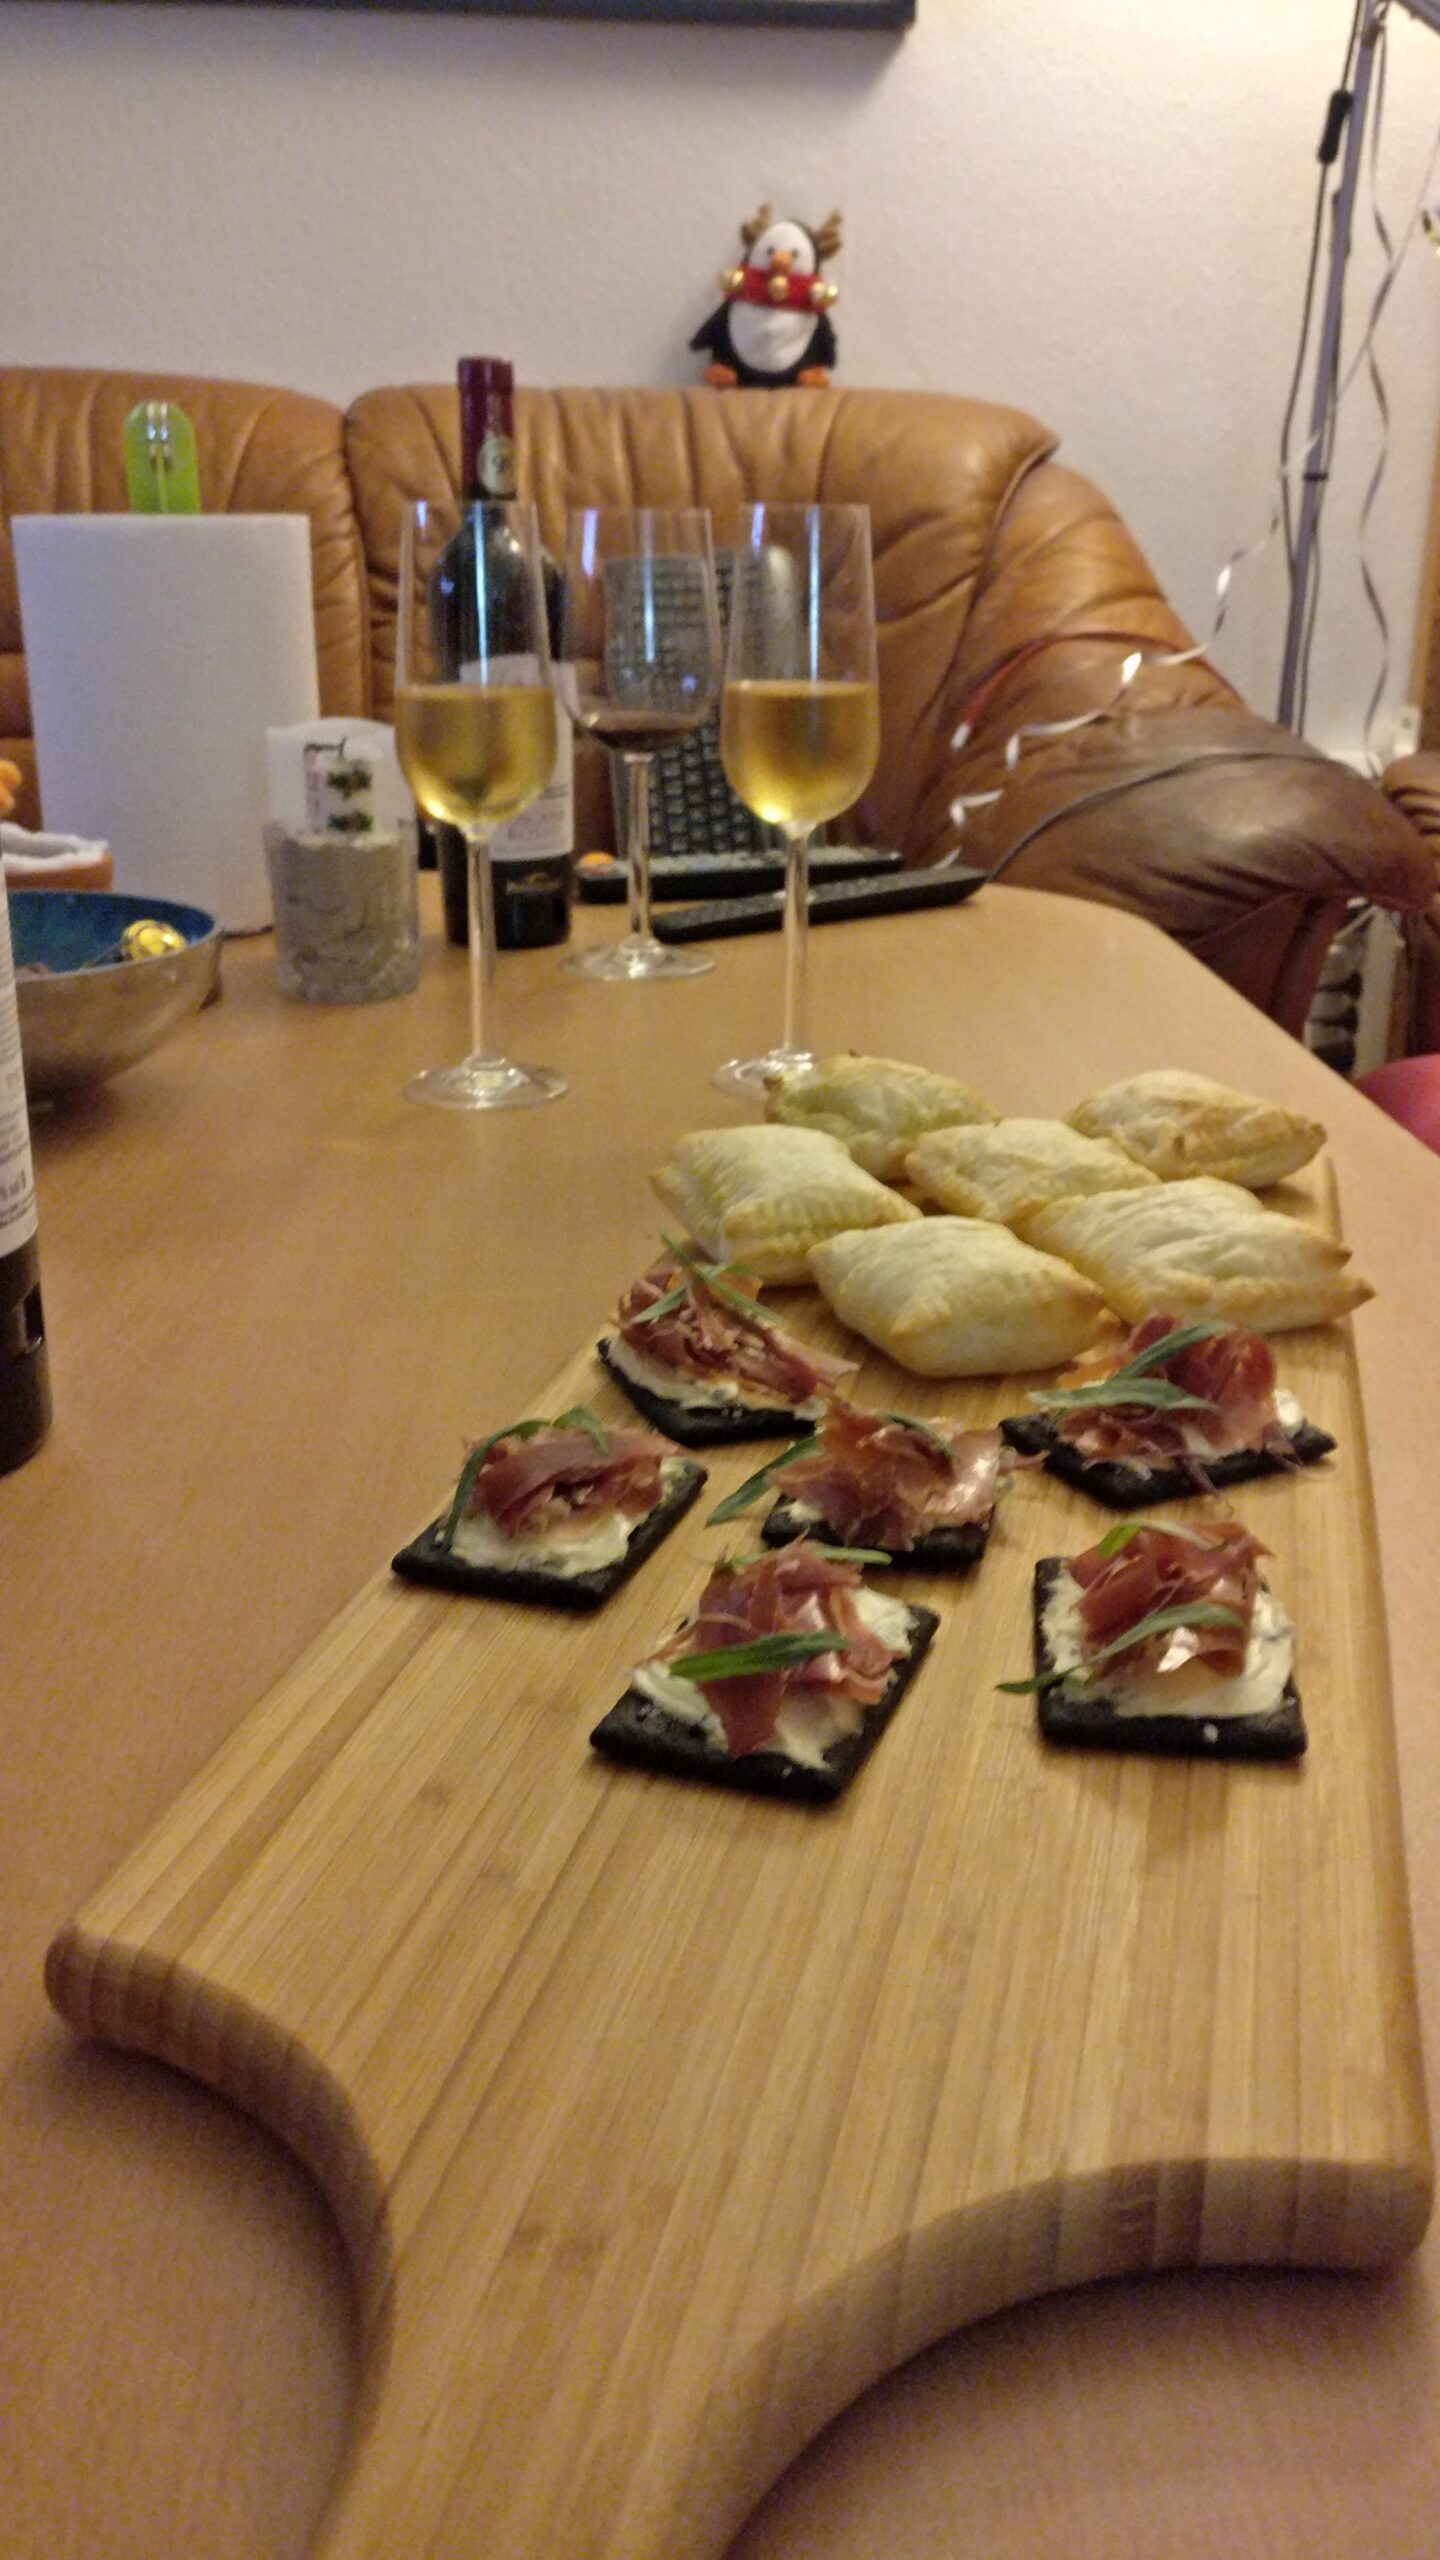
\includegraphics{rmds/images/snacks-scaled.jpg}

Smørgederne er de letteste. En skive gedeost fra en gederulle. Placeret
oven på en firkant butterdej. En lille teskefuld grøn pesto oven på
osten. Pakkes ind i butterdej, bages i ovnen ved 200 grader i ca. 7
minutter. Hold øje med dem!

Skinken på bearnaise er sådan set også ret lette, men der er flere
ingredienser. Flødeost røres med lidt sød sennep og friskhakket
estragon. Det smøres på en lille kiks. Jeg havde valgt ``dark sky''
kiksene fra Bisca - de laves på Møn, hvor vi holdt sommerferie i dette
pestår. Og de var lidt for store. Gå efter noget der er lidt mindre, for
de bør spises i en mundfuld.

Serrano skinke skæres i passende stykker og anrettes oven på kiksen, og
der placeres et par blade frisk estragon ovenpå. Nam!

\bookmarksetup{startatroot}

\hypertarget{bagning-1}{%
\chapter{Bagning}\label{bagning-1}}

\hypertarget{koldhuxe6vede-morgenboller-1}{%
\section{Koldhævede morgenboller}\label{koldhuxe6vede-morgenboller-1}}

Goto opskriften, fordi den kan røres sammen aftenen i forvejen.

\begin{itemize}
\tightlist
\item
  6 dl vand
\item
  25 g gær
\item
  15 gram akaciehonning
\item
  480 gram hvedemel
\item
  65 gram solsikkekerner
\item
  270 gram durummel
\item
  2 tsk salt
\end{itemize}

Rør gæren ud i vandet. Rør honningen ud i gærblandingen

Bland kerner og hvedemel.

Bland salt og durummel (tipo 00 fungerer også fint).

Rør durummel i gærblandingen. Rør hvedemel i dejen.

Rør sammen til dejen er jævn, klæg, og har en skinnende/våd overflade

Hæver tildækket to timer på køkkenbordet, eller natten over på køl.

Forvarm ovnen til 225 grader varmluft. Sæt bollerne på to plader, 8 på
hver. Gør det med våde hænder.

Bages ca. 17 minutter, til de har en let gylden overflade.

Dette er en god basis opskrift. Der kan hældes flere/færre/andre kerner
i. Eller der kan tilsættes havregryn eller grovere mel i - i så fald
skal der formentlig lidt mere væske i, da havregryn eller groft mel
suger mere væske.

\hypertarget{fuglebruxf8d-1}{%
\section{fuglebrød}\label{fuglebruxf8d-1}}

Almindelig brøddej. Og så formet på denne måde:
\includegraphics{rmds/images/fuglebrød.jpg} Gerne en lille rosin eller
korender som øje.

\hypertarget{finsk-bruxf8d-1}{%
\section{Finsk Brød}\label{finsk-bruxf8d-1}}

Fra - ja hun var vel en slags tante. På min fars side.

\begin{itemize}
\tightlist
\item
  175 gram hvedemel
\item
  125 gram margarine
\item
  50 gram stødt melis
\end{itemize}

Pensles med æg, og drysses med perlesukker. Og bages til de er
lysebrune.

Ja, det er altså det fulde omfang af tante Metas opskrift. Det er
selvfølgelig udfordringen når man får fat i opskrifter fra erfarne
husmødre. Heldigvis kan jeg trække på min mors praksis.

Margarinen - jeg ville jo nok vælge smør i stedet, smuldres i melet,
sukker røres i. Og dejen hviler. Den rulles ud i stænger af 2½ cm
tykkelse, og trykkes lidt flade. De skæres ud i stykker af 3-4 cm
længde. Sådan lidt rhombeformede.

Temperaturen i ovnen skal være 200 grader. Og det tager en ti minutters
tid før de er lysebrune.

\hypertarget{klejner---mors-opskrift-1}{%
\section{Klejner - mors opskrift}\label{klejner---mors-opskrift-1}}

Denne opskrift har så ikke gået så meget i arv. Endnu. Det er godt nok
mors opskrift, men hun fik den af en ældre dame hun gik til knipling med
en gang i tidernes morgen. Så den er ikke helt ung. Og nu er den så gået
i arv fra mor til hendes sønner. Hvis min lillebror får taget sig sammen
til at producere nogen nevøer og niecer, kan den gå i arv til dem.

Ingredienser:

\begin{itemize}
\tightlist
\item
  188 g sukker
\item
  100 gram margarine
\item
  3 æg
\item
  2 spsk mælk
\item
  Revet skal, og saft, af ½ citron
\item
  400 gram mel
\end{itemize}

Fremgangsmåde:

Pisk sukker og margarine (jeg bruger smør i stedet) sammen. Pisk æg,
mælk og citron i. Ælt herefter mel i.

Rul dejen ud til ca. 3 millimeters tykkelse, kør klejnejernet over, vrid
klejnerne og kog dem i palmin. Palminen skal op omkring de 180 grader.
Stik enden af en tændstik i - når det begynder at syde og boble godt
omkring den, er olien klar.

Jeg ved ikke om man havde en anden slags mel i gamle dage, eller om
æggene var specielt små. Men jeg ender altid med at skulle have en del
ekstra mel i. Og det var også min mors erfaring.

\hypertarget{brune-kager---mors-opskrift-1}{%
\section{Brune kager - mors
opskrift}\label{brune-kager---mors-opskrift-1}}

Der er opskrifter der går i arv - og de er ofte knyttet til julen.

Dette er familiens opskrift på brune kager. Og den er faktisk af ældre
dato. Fortællingen går på at min mors fastre, altså min morfars søstre,
ikke ville udlevere den til min mormor. Det var familiens hemmelige
brunkageopskrift, der stammede fra min oldemor på min morfars side, fra
Langeland.

Meget hemmelig.

Så nu lægger jeg den på internettet\ldots{}

\begin{itemize}
\tightlist
\item
  ½ kg margarine
\item
  ½ kg sukker
\item
  1/4 kg sirup
\end{itemize}

Varmes op til kogepunktet, og tages af varmen.

\begin{itemize}
\tightlist
\item
  15 gram potaske udrøres i 1 spsk koldt vand, og hældes i gryden. Der
  røres til det bruser op.
\item
  150 gram smuttede og hakkede mandler
\item
  50 gram sukat
\item
  3-5 tsk. kanel
\item
  3 tsk stødte nelliker
\item
  2 tsk ingefær
\item
  50 gram pomeransskal
\end{itemize}

Hældes i gryden, og der røres. Når det er kølet lidt af, æltes 1 kg
hvedemel i massen. Når den er blevet så koldt at man kan arbejde med
den, rulles dejen ud i pølser i en tykkelse der matcher den diameter man
ønsker at kagerne skal have.

Rul pølserne ind i bagepapir, og læg dem i køleskabet. Roter pølserne,
så de forbliver runde.

Skær dem tyndt ud (brug en god skarp brødkniv), og bag dem ved 175-180
grader i 8 minutter. Mors opskrift siger 6 minutter, det holdt ikke i
min ovn.

Dette er den traumatiske julekage i vores familie. Dejen kan nemlig være
ret drilsk, og smuldrer let når man skærer. Mange aftener har min mor
stået og lagt dejstumper sammen i puslespil.

Det problem havde jeg ikke helt. Jeg ved ikke om det var begynderheld,
eller fordi jeg ikke holdt mig helt til opskriften. Jeg brugte smør i
stedet for margarine,~ baseret på en teori om at de nok ikke havde
margarine på Langeland på min oldemors tid. Det kunne de nok have, hun
må være født lige i slutningen af 1800-tallet, og margarinen er fra
sidste halvdel af samme. Men hvis den vitterligt har gået i arv siden
før hendes fødsel, så er det ret sandsynligt at den oprindeligt har
brugt smør.

Anyway, det gik forbløffende smertefrit. Nu skal vi bare forsøge at få
dem til at holde hele vejen til juleaften.

\hypertarget{vanillekranse---mors-opskrift-1}{%
\section{Vanillekranse - mors
opskrift}\label{vanillekranse---mors-opskrift-1}}

\begin{itemize}
\tightlist
\item
  250 g mel
\item
  200 g smør
\item
  150 g sukker
\item
  60 g finthakkede mandler
\item
  kornene fra ½ stang vanille
\item
  1/2 æg
\end{itemize}

Smørret smuldres i melet. Resten af de tørre ingredienser blandes i, og
samles med ægget.

Extruderes på kødhakker, med stjernehul, og samles til kranse. En
passende længde pølse til en krans er 8-9 cm. Eller ca. 4 fingres
bredde, afhængig af hvor fede fingre man har. Bages ved 200 grader i
7-10 minutter.

Dette er mors standardopskrift, og standardportionsstørrelse. Jeg synes
roligt man kan bage dobbelt portion. Så skal man heller ikke bøvle med
halve æg.

Og så var vanillestænger dyre engang. De er sådan set ikke blevet
billigere. Men man kan roligt hælde mere vanille i.~ Meget mere! En af
de nærmeste dage bager jeg dobbelt portion, og regner med at bruge 4
stænger.

\hypertarget{ruxf8rt-kage-med-marmelade-1}{%
\section{Rørt kage med marmelade}\label{ruxf8rt-kage-med-marmelade-1}}

I serien ``Metas opskrifter'' er vi nået til kager.

Opskriften bærer præg af en noget mere beskeden husholdning end den
gennemsnitlige danske i dag. * 3 hele æg * 250-400 gram sukker * 250
gram valsede byggryn * 250 gram rugsigtemel * 2 dl fløde eller mælk * 2
dl vand * 1 bagepulver (et brev, red.) * 1-2 kopper syltetøj eller
marmelade

Slå æggene i en skål. Kom sukkeret deri, efter hvad man kan ofre og som
det tiltrænges i forhold til syltetøjet der skal i. Pisk det godt
sammen. Lad byggrynene gå en gang gennem kødmaskinen så får de en
konsistens af mel. Bland gryn, mel og bagepulver sammen. Syltetøjet som
kan være stikkelsbær, kirsebær blommer hvoraf stenene er taget ud,
syltet græskar, grønne tomater eller lignende skåret småt, kommes i de
røte æg, og blandes forsigtigt godt deri. Bagefter tilsættes det
sammenblandede mel og mælken skiftevis hvorefter dejgen fyldes i en
velsmurt form og bages 3/4 time. Frugtstykkerne i kagen virker som
rosiner og sukat, og fugtigheden fra syltetøjet bevirker, at kagen ikke
bliver tør. Den er bedst når den har stået et par dage før den spises.

Meta har noteret, at opskriften er fra Familie-Journalen.

\hypertarget{japanske-boller-1}{%
\section{Japanske boller}\label{japanske-boller-1}}

Jeg har et par gode bolle-opskrifter i kogebogen.~ Den her fx. ~Men
forleden faldt jeg over en anden. Den baserer sig angiveligt på en eller
anden japansk teknik. Og kaldes Tang-Zhong. Konceptet er at der først
koges en jævning af dele af melet og væsken. Det skulle gøre det muligt
at holde bedre på fugten i bollen eller brødet, og betyde at bagværket
er friskt, saftigt og lækker i op til en uge.

Det lever den dog ikke helt op til. De 20 boller der kom ud af
opskriften, var væk allerede tre dage efter de blev bagt. For selv om de
ikke var så lækre efter tre dage, som de var da de kom ud af ovnen, var
de stadig bedre end en standard brioche efter tre timer.

Ingredienser

\begin{itemize}
\tightlist
\item
  6 dl mælk
\item
  800 gram mel
\item
  25 gram gær
\item
  ½ tsk salt
\item
  4 spsk sukker
\item
  1 æg
\item
  150 gram smør.
\end{itemize}

Fremgangsmåde

Kog jævning af 40 gram mel og 2 dl mel. Rør det godt sammen i en
kasserolle, og bring det i kog - rør godt undervejs. Det bliver tykt!
Lun 4 dl mælk, og rør gæren ud. Lad jævningen køle af, og rør den sammen
med alle andre ingredienser end smørret. Tilsæt smørret i små stykker,
og rør videre til dejen slipper skålen. Vej bollerne af i portioner af
ca. 80 gram, form dem til boller og placer dem på bagepladen. Lad
bollerne hæve 1½ time under et viskestykke. Pensl bollerne (jeg bruger
mælk eller æg), og bag dem ved 200 grader i 12-15 minutter.

\hypertarget{fastelavnsboller-1}{%
\section{Fastelavnsboller}\label{fastelavnsboller-1}}

Forstanderindens (forbedrede) fastelavnsboller.

Dejen

100 gram smør, smeltet 2 dl lun mælk (gerne sødmælk) 25 gram gær 50 gram
rørsukker 1 tsk salt 1 æg 1/ 2 kilo hvedemel Gæren røres ud i mælken,
sukker, salt og smør, som ikke må være alt for varmt, tilsættes. Melet
æltes i lidt ad gangen. Hold lidt tilbage, dejen skal være blød og
spændstig, ikke hård og tør. Dejen hæver til ca. dobbelt størrelse under
et viskestykke. Det tager en god times tid i et lunt køkken.

Mens dejen hæver, laver man cremen.

Cremen

2,5 dl fløde 2,5 dl sødmælk (jo!) 100 gram sukker 1 stang vanilje 6
æggeblommer 30 gram maizena Æggeblommerne piskes sammen med sukker,
maizena og kornene fra vaniljestangen. Mælk og fløde koges op sammen med
den tomme vaniljestang. Når blandingen koger, hældes den i æggemassen.
Cremen skal være tyk som en solid bearnaisecreme, og det bliver den
næppe af at hælde den kogende fløde over æggeblommerne, så hæld massen
tilbage i gryden og kog den op. Rør som besat imens. Hvis den klumper,
kan den reddes med en elpisker. Køl cremen af. Hvis man hælder den i en
skål eller bøtte, køler den hurtigere, end hvis den bliver stående i
gryden.

Jeg synes, det er lækkert også at komme remonce i - lidt til den vamle
side, men klart lækkert, selv om det ikke indgår i den oprindelige
opskrift. Man kan eventuelt halvere opskriften på remonce og lave
halvdelen med og halvdelen uden og lave sammenlignende studier.

Remoncen

100 gram marcipan 100 gram rørsukker 100 gram smør Den oprindelige
opskrift foreslår, at man nu bare ruller dejen ud, men jeg synes, den
bliver endnu bedre, hvis man ruller smør i den (men hvis du bliver
livstræt bare ved tanken, så spring over og gå direkte til udrulningen -
de smager godt uden, men endnu bedre med).

Smør i dejen

100 gram blødt smør Dejen rulles ud til et rektangel, ca. 40 gange 50
cm. Smør smørret på, fold dejen sammen, først på langs og så på tværs,
så den ligger i fire lag (som du ville folde en vaskeklud).

Rul dejen ud igen, så den er så tynd som mulig, optimalt 30 gange 60 cm,
realistisk nok lidt mindre. Brug så lidt mel som muligt, men nok til at
dejen ikke hænger fast i alt, og at du får et hjerteslag af raseri.

Dejen skæres i stykker på 10 gange 10 cm.

Hvis du ikke fik rullet dejen tyndt nok, kan du eventuelt lige rulle
hvert stykke lidt ekstra.

Læg en pæn klat creme på hvert stykke - og en skefuld remonce, hvis du
er til den slags. Fold bollerne ved først at klemme de fire spidser
sammen, så siderne. Vær omhyggelig.

Lad de små pakker hæve ca. 20 minutter.

Pensles med æg.

Bages ved 225 grader i ca. 10-12 min. De skal være smukt brune, men ikke
hårde.

Chokoladen

100 gram mørk chokolade ½ dl fløde Smelt chokoladen, kom fløde i. Den må
godt være ret tyk. Når bollerne er kølet lidt af, pensles de med
chokoladen.

Man kan også fylde bollerne med flødeskum.

De skal være HELT kolde, ellers smelter fløden.

Hvis man har en sprøjtetylle, laver man et lille hul og sprøjter det ind
i bollen. Ellers skærer man over og lægger sammen. Har man creme
tilovers, som man ikke fik mast ind i bollerne, kan man også lave
konditorcreme, hvor man blander flødeskum og cremen (pisk den først, så
den er helt glat). Det smager også godt i fastelavnsboller.

Spiser man mere end tre på en eftermiddag, har man svært ved at spise
aftensmad.

\hypertarget{muxf8rdej-1}{%
\section{Mørdej}\label{muxf8rdej-1}}

Standard mørdej. Den er god.

\begin{itemize}
\tightlist
\item
  75 g blødt smør
\item
  50 g flormelis
\item
  1⁄2 sammenpisket æg
\item
  10 g mandelmel
\item
  125 g hvedemel
\item
  1 lille nip salt
\end{itemize}

Rør smør og sukker blødt med elpiskeren. Tilsæt ægget, og pisk det ind.

Tilsæt dernæst mel og salt. Når dejen hænger sammen stopper du med at
røre, og samler dejen med hænderne.

Den vil være lettere at arbejde med hvis den får en tur i køleskabet
først.

\hypertarget{jordnuxf8dde-chokolade-smuxe5kager-1}{%
\section{Jordnødde-chokolade
småkager}\label{jordnuxf8dde-chokolade-smuxe5kager-1}}

Eller vel egentlig cookies.

Ingredienser:

\begin{itemize}
\tightlist
\item
  250 gram smooth jordnøddesmør
\item
  100 gram sukker (gerne noget lys muscovado sukker
\item
  80 gram mørk chokolade
\item
  1 tsk vanillesukker
\item
  1 æg
\item
  Et nip salt
\end{itemize}

Procedure

Rør æg og sukker sammen til æggesnaps. Tilsæt resten af ingredienserne
(bortset fra chokoladen), og rør sammen til dejen er homogen. Hak
chokoladen og vend den i dejen. Tril dejen ud i 12 kugler, læg dem på
bagepladen (kom noget bagepapir på først) og tryk dem flade
\textasciitilde{} ½ cm tykkelse. Som med de fleste andre småkager flyder
de ud, så giv dem god plads på pladen. Bag dem i en forvarmet ovn (160
grader) i 25-30 minutter. De er fine efter 20, men ret bløde. Som for
alle andre småkager gælder det at de bliver hårdere når de køler af
(fedtstoffet bliver ganske enkelt stivere).

Opskriften er nappet fra Sabine Murati.~ Man kan med fordel besøge
hendes hjemmeside, for der er flere og bedre opskrifter end jeg har her.
Den er dog justeret lidt. Kemikeren her synes ikke der er nogen grund
til at bruge himalaya-salt. Himalaya salt er grundlæggende snavset salt,
og ethvert postulat om helsebringende effekter er det vi med et
fagudtryk kalder for ``vrøvl''. Og hvis man virkelig er bekymret for
økologi og sådan noget, så bør man måske også overveje om man bør bruge
salt der er blevet transportet 6.900 kilometer, for at nå frem til
køkkenet i Rødovre. Eller om man kunne klare sig med noget der er
transporteret 358 kilometer fra Mariager Fjord. Jeg har også erstattet
kokos-sukkeret med almindeligt sukker. Hvis vi godt vil tænke lidt over
klima og den slags, tror jeg også almindeligt sukker fra Lolland sviner
en del mindre, end kokossukker der skal tranporteres fra
Indonesien\ldots{}

Nåja, de smagte godt. Men næste gang lader jeg være med at gå efter 80\%
chokolade. Det var for bittert.

\hypertarget{abrikostuxe6rte-1}{%
\section{Abrikostærte}\label{abrikostuxe6rte-1}}

Der skal bruges en portion mørdej.~ Rul dejen ud mellem to stykker
bagepapir. Den skal være cirkelformet, og passe til en tærteform - min
er 24 cm i diameter.

Løft dejen over i formen, og tryk den af i kanterne. Prik dejen med en
gaffel. Eller sådan et hjul med pigge.

Så skal der fyld i!

\begin{itemize}
\tightlist
\item
  14 friske abrikoser i kvarte
\item
  saft af 1/2 citron
\item
  2-3 tsk amaretto
\item
  1 stang vanilje
\item
  150 g sukker
\item
  3 spsk. maizena
\end{itemize}

Vask og kvarter abrikoserne. Læg dem i en skål og vend dem med citrosaft
og amaretto. Det er tilladt at smage på den inden, så du er sikker på at
den ikke er blevet dårlig.

Flæk vanillestangen og fordel kornene i sukkert. Bland vanillesukker og
maizena i en separat skål.

Saml det hele i en skål, og bred fyldet ud i tærtebunden.

Bag dyret i 20 minutter ved 220°C, skru ned til 190°C og bag videre i
30-40 minutter. Det er helt fint hvis abrikoserne tager lidt farve.

\hypertarget{pebernuxf8dder---mors-opskrift-1}{%
\section{Pebernødder - mors
opskrift}\label{pebernuxf8dder---mors-opskrift-1}}

Pebernødder. Det er nok min foretrukne julesmåkage. Altså i den udgave
som min mor laver den. Dem man køber i supermarkedet er vist lavet på
samme dej som deres brunkager. Den er ærligt talt lidt kedelig. Men
mors! De er gode.

Opskriften har været i familien i nogen år, men er vist ikke den ældste
vi har. Den stammer vistnok fra mormors kogebog, og er derfor fra kort
efter besættelsen. Så den er ikke nødvendigvis ret meget mere end 70-75
år gammel.

Man tager:

\begin{itemize}
\tightlist
\item
  500 g hvedemel
\item
  250 g sukker
\item
  1 tsk hortetakssalt
\item
  1 toppet tsk kanel
\item
  1 toppet tsk ingefær
\item
  1 toppet tsk kardemomme
\item
  1/4 tsk hvid peber
\item
  125 gram smør
\item
  Revet skal af en citron
\item
  2 æg
\end{itemize}

Først nuldre smørret ud i melet. Mor brugte vist oprindeligt margarine.
Jeg er ikke helt sikker på at det er sundere end smør. Så her i huset er
det altså smør. Sukkeret blandes med hjortetakssaltet, krydderierne og
citronskallen, og blandes i mel/smør blandingen.

Dejen samles med to sammenpiskede æg. Det er utroligt hårdt arbejde og
tager en del længere tid end man lige tror. Jeg plejer at lave af to
kilo mel, altså firedobbelt portion, og det gik lidt lettere da jeg i år
(2017) skruede mængden af æg op fra 8 til 9.

Dejen trilles i små kugler. Sådan ca. et par centimeter i diameter,
afhængig af tålmodighed, og hvor store nødder man ønsker sig til jul.
Bages i ca. 12 minutter ved 180 grader. I min ovn skal de have lidt
længere. Og så spreder der sig en liflig duft af herretoilet i hele
køkkenet. Hjortetakssalt er ammoniumhydrogencarbonat. Så under bagningen
frigives der ammnoniak. Luft ud hvis det bliver et problem, nødderne
kommer ikke til at smage af det.

\hypertarget{kagefigurer-1}{%
\section{Kagefigurer}\label{kagefigurer-1}}

Normalt laver jeg kagefigurer af en brunkagelignende dej. Men jeg kunne
godt tænke mig en lysere udgave. Og gerne en der er mere robust i formen
når den bages.

The Decorated Cookie har en opskrift, der ikke er så ringe endda. Men
som selvfølgelig skal oversættes til fornuftige SI-enheder. Og justeres
lidt.

225 gram smør 115 gram flormelis 1 æg 1 tsk vanillepasta. Eller en spsk
vanillesukker 300 gram mel ½ tsk fint salt

Der kan suppleres med mandelekstrakt, eller andre smagsgivere. 1-2
teskeer. Men det er en smagssag.

Sigt salt og mel sammen.

Rør smør og sukker sammen til blandingen er luftig. Det tager en krig.
Tilsæt ægget og rør godt. Vanillepasta og eventuelle andre smagsgivere
tilsættes.~ Rør melblandingen i lidt af gangen.

Afkøl dejen i køleskab et par timer. Gerne i en frysepose hvor den er
trykket flad, det sparer tid når den skal rulles ud.

Rul dejen ud til ca. 5 millimeters tykkelse, stik figurerne ud og bag
dem i en forvarmet ovn ved 190 grader i 12-14 minutter. Eller i min ovn
nok snarere 11-12 minutter ved 200 grader. Det afhænger af størrelsen,
men de er færdige når kanterne er blevet lysebrune.

\hypertarget{chokolade-sifon-kage-2}{%
\section{Chokolade sifon kage}\label{chokolade-sifon-kage-2}}

Det lykkedes ikke at finde majsjuice. Thaiforretningerne nede ved
Istedgade har mange andre interessante produkter, men ikke majsjuice.

Så i stedet lavede jeg denne:

110 g mørk chokolade 5 mindre æg 3 spsk mel 6 spsk sukker

Chokoladen smeltes, og resten røres i. Det hele filtreres og hældes på
sifonen. To kapsler lattergas tilsættes. Den anden blev ikke tømt helt i
sifonen.

Der omrystes, og sprøjtes i ramekinerne (teflonbelagte), og en ramekin
af gangen gives 30-45 sekunder i mikroovnen ved 900 W. Bemærk at
ramekinen ikke er specielt varm efter første omgang. Men efter anden er
den varmet op, tredie gang den har været i ovnen er den varm, selv for
en kemiker. Hold godt øje med kagen i ovnen. Den får hurtigt for meget.

Det er ikke sundt, men det smager godt, og så her det stor nørdværdi.
Opskriften er tyvstjålet fra:
http://projects.washingtonpost.com/recipes/2010/12/01/30-second-chocolate-cake/~med
lette modificeringer.

http://projects.washingtonpost.com/recipes/2010/12/01/30-second-chocolate-cake/

\hypertarget{sandkage-1}{%
\section{Sandkage}\label{sandkage-1}}

½ pund margarine røres med ½ pund stødt melis. Der røres fem æggeblommer
i. og ½ pund mel. 5 stift piskede æggehvider vendes i. En af metas
opskrifter

\hypertarget{verdens-bedste-kringle-1}{%
\section{Verdens bedste kringle}\label{verdens-bedste-kringle-1}}

Opskriften er tyvstjålet fra Politiken. Men den er på prosaform, og det
er lidt bøvlet når man skal fremstille den. Oprindeligt er det den Søren
Ryge gjorde kendt.

Dej:

50 g gær 1 kop lunkent vand Lidt salt 3 spsk sukker 3 æg 330 g margarine
450 g mel

Remonce:

225 g sukker 225 g margarine Kardemomme eller kanel

I øvrigt:

Rosiner, perlesukker og hakkede nødder.

Fremgangsmåde:

Gæren smuldres ud i vandet, og sukker samt æg tilsættes. Margarinen
skæres i stykker og smuldres i. Skålen sættes lunt og gærer i en halv
time. Mel tilsættes og der æltes. Den oprindelige opskrift taler om at
bruge fingrene og noget om erfaring og den slags. Det er lidt Søren Ryge
agtigt, men det giver god mening. Margarinen behøver ikke at blive helt
fordelt. Dejen hæver mindst en time, og røres ud til et 50-70 cm. langt
stykke, højest 3 mm tykt. Der foldes og rulles, gentagne gange, tilsæt
evt. ekstra mel. Dejen skæresi 4 stykker, ca. 15 cm brede. Remoncen
fremstilles:; Sukker og margarine, og krydderi, varmes i gryde til den
er tyktflydende. Remoncen hældes ud på de fire stænger, der hældes
rigeligt rosiner på, og dejen foldes sammen. Kringlerne løftes over i en
bradepande, og pensles med æg. Der efterhæves i en halv time. Der
pensles med æg, og drysses med sukker og hakkede nødder Bages i
forvarmet ovn. Start ved 225 grader og sæt ned til 200 grader. Samlet
bagetid 14-16 minutter.

\hypertarget{baba-au-ruhm-1}{%
\section{Baba au ruhm}\label{baba-au-ruhm-1}}

https://www.dr.dk/mad/opskrift/baba-au-ruhm

\hypertarget{en-god-ung-mand---chokoladedessert-1}{%
\section{En god ung mand -
chokoladedessert}\label{en-god-ung-mand---chokoladedessert-1}}

Regeringen har meget på samvittigheden. Men det frankofile madprogram på
Radio 247, Croque Monsieur var nok stoppet med Master Fatmans død under
alle omstændigheder.

Det er her jeg har opskriften fra. Jeg tillader mig at stjæle den ret
direkte - det er trods alt en standardopskrift af ældre dato fra det
franske køkken.

Dér hedder den ``Un bon jeune homme''. Og her i køkkenet kan vi godt
lide gode unge mænd. Så længe de enten tier stille, eller er gamle nok
til at de ikke er ulidelige at høre på.

Man tager:

7 dl mælk 50 gram sukker 175 god mørk chokolade, sådan en 65\% sag

Og så gør man følgende:

Mælken hældes i en tykbundet gryde, sammen med sukkeret, og bringes
langsomt i kog på mellemvarme. Mens man venter på at den kommer i kog,
hakkes chokoladen groft. Den tilsættes når mælken koger. Og så røres der
mens blandingen simrer ved lav varme. I 45 minutter. Det starter som
varm chokolade, men efterhånden som vandet fordamper, cremer chokoladen
blandingen, og det ender med at være en relativt tyk creme. Gryner
cremen får den en omgang med stavblenderen. Derefter hældes cremen i 4
ramekiner, og sættes på køl til den er kold. Server evt med flødeskum
eller en kold creme anglaise.

\hypertarget{langtidshuxe6vede-bruxf8d-1}{%
\section{Langtidshævede brød}\label{langtidshuxe6vede-bruxf8d-1}}

Indlæg fera 23. marts 2020 - hvor pesten rasede\ldots{}

Zombie-apokalypsen er lige rundt om hjørnet. Om en måned finder vi ud af
at alle de der blev ``raske'' efter Corona/Covid19/Kinesisk Influenza,
forvandles til hjerneædende zombier.

Så vi kan lige så godt få sat en surdej over, så vi kan bage brød når
nationen løber tør for gær.

Indtil da, her er opskriften på to lækre brød bagt med minimale mængder
gær.

5 g gær 1 tsk sukker 4 dl lunkent vand 450 g mel 1 tsk salt

Rør gær og sukker ud i vandet. Tilsæt mel og rør til det er blandet godt
op til en jævn konsistens uden klumper.

Lad hæve i mindst 7 timer på køkkenbordet. Helst under film, så der ikke
er for megen fordampning.

Skrab dejen ud på køkkenbordet. Husk at strø pænt med mel på bordet
først. Den er pænt flydende. Det er meningen.

Drys dejen med mel, og fold den ind over sig selv en 4-5 gange. Ikke
noget med at ælte! Del den i to, flyt dem over på en bageplade (med
bagepapir) - sådan nogenlunde brødformede. Smid det hele i en forvarmet
ovn (250 grader varmluft) i 10 minutter. Skru varmen ned til 225 grader,
og giv dem yderligere 10 minutter.

Lad dem køle af på en rist i 30 minutter.

Jeg har ikke lige nogen billeder af resultatet. De blev spist for
hurtigt, men prøver at nå det i næste omgang.

\hypertarget{surdejsboller-1}{%
\section{Surdejsboller}\label{surdejsboller-1}}

Bent Surdej kan nu også lave boller. Jeg ved ikke helt hvorfor, men
efter den første coronanedlukning er overstået, har han tilbragt mere af
tiden i køleskabet. Og det er han glad for. Så nu kan der også leveres
boller.

Discardet fra Bent. 2-2½ dl af det jeg ellers ville have hældt i vasken
ved fodringen. 450 gram mel 18 gram fint salt 3 dl vand En sjat
olivenolie

Kl 630 eller deromkring går jeg i gang. Bland salt og mel, og ælt det
hele sammen. Det er lidt vigtigt ikke at hælde salt direkte i surdejen,
det slår den ihjel.

Så lader jeg dejen hæve under et viskestykke til jeg kommer hjem fra
arbejde omkring kl. 16. Ovnen med tilhørende bagestål varmes op til 250
grader varmluft. Med lidt held har min mand tændt den inden jeg kommer
hjem. Han er nemlig blevet hjemsendt igen.

Dejen hakkes ud i 8 stykker, løftes over på bagepapir, og skubbes ind på
bagestålet. Og så skal de bare have til de er lysebrune på overfladen.

Og det er det. Jeg er godt tilfreds med resultatet, de smager lige så
godt som Lagkagehusets surdejsboller. Og koster en brøkdel.

\hypertarget{boller-1}{%
\section{Boller}\label{boller-1}}

Årsagen til at dele af svigermekanikken mener jeg er den store
bagermester er denne opskrift på bløde fødselsdagsboller:

http://www.dk-kogebogen.dk/opskrift2/visopskrift.php?id=26732

\hypertarget{juxf8dekager---mors-opskrift-1}{%
\section{Jødekager - mors
opskrift}\label{juxf8dekager---mors-opskrift-1}}

Så\ldots{} Vi skal nok have den rekvireret fra mor\ldots.

\bookmarksetup{startatroot}

\hypertarget{references}{%
\chapter*{References}\label{references}}
\addcontentsline{toc}{chapter}{References}

\markboth{References}{References}

\hypertarget{refs}{}
\begin{CSLReferences}{1}{0}
\leavevmode\vadjust pre{\hypertarget{ref-knuth84}{}}%
Knuth, Donald E. 1984. {``Literate Programming.''} \emph{Comput. J.} 27
(2): 97--111. \url{https://doi.org/10.1093/comjnl/27.2.97}.

\end{CSLReferences}



\end{document}
